
\section{Results and discussion}
\label{sec:results}


For each dataset, the combination of a probabilistic degradation model and the SR model (from now on, a pipeline) was trained. 
Each pipeline has three main components: A generator used to create LR images aligned with the target domain from HR images coming from the source domain. A discriminator used to distinguish between authentic LR images coming from the target domain and the generated ones, and an SR model used to improve the resolution of the generated LR images during training.


The pipeline trained on $\mathcal{D}_{\text{SF}-\text{SF}}$, using unpaired HR-LR pairs generated by applying the baseline degradation model described in \ref{fig:3-probabilistic-degradation-model}, will be referred to as the baseline pipeline.
While the employed degradation model is stochastic, it has known parameters that are very close to bicubic downsampling + white noise. The objective is to observe how the GAN is able to imitate a known degradation model in order to produce LR images.

The pipeline trained on $\mathcal{D}_{\text{SF}-\text{RF}}$, using unpaired synthetic HR and real LR FOREST-2 images, will be referred to as the adapted pipeline.
In this case, the degradation model is unknown, and the objective of the GAN is to estimate it by generating LR images that come from the same distribution as the real FOREST-2 images.

    \subsection{Source domain}

        This subsection will analyze the results from the experiments performed on the source domain.
        The process consists of degrading the synthetic HR FOREST-2 images using the probabilistic degradation model trained through adversarial learning and then super resolving its output.
        This is the equivalent of the black arrows flow described in Fig. \ref{fig:3-GAN-degradation-model}. 
        As in this case the ground truth is known, the performance of the super resolution can be evaluated using metrics like PSNR and SSIM. 

        Fig. \ref{fig:5-source_domain_sample} shows the results of the baseline and the adapted pipeline when applied to one sample from the source domain. For comparison, a pipeline consisting of simple bicubic downsampling + white noise for degradation and bicubic upsampling for SR is also shown. 
        While the baseline kernel is very simple, and the noise is more or less uniform across the image, the adapted kernel is more complex, and its noise seems to be strongly correlated with the pixel intensity.

        The degraded LR images present considerable differences. While the baseline pipeline produces images very similar to the bicubic downsampling + white noise LR reference,
        the adapted pipeline produces blurrier images with more noise, suggesting that FOREST-2 delivers scenes with less resolution than what was initially expected. 
        This is also confirmed by calculating the PSNR between the LR image generated by each pipeline with the bicubic downsampling + white noise LR reference, which yields worse results for the adapted pipeline.
        
        Despite having very different starting points, the SR images produced by both pipelines yield better performance than bicubic interpolation, and are very similar to each other. This suggests that the super resolution model is able to recover the details lost during a more complex degradation process.

        
        \begin{figure}[H]
            \centering

            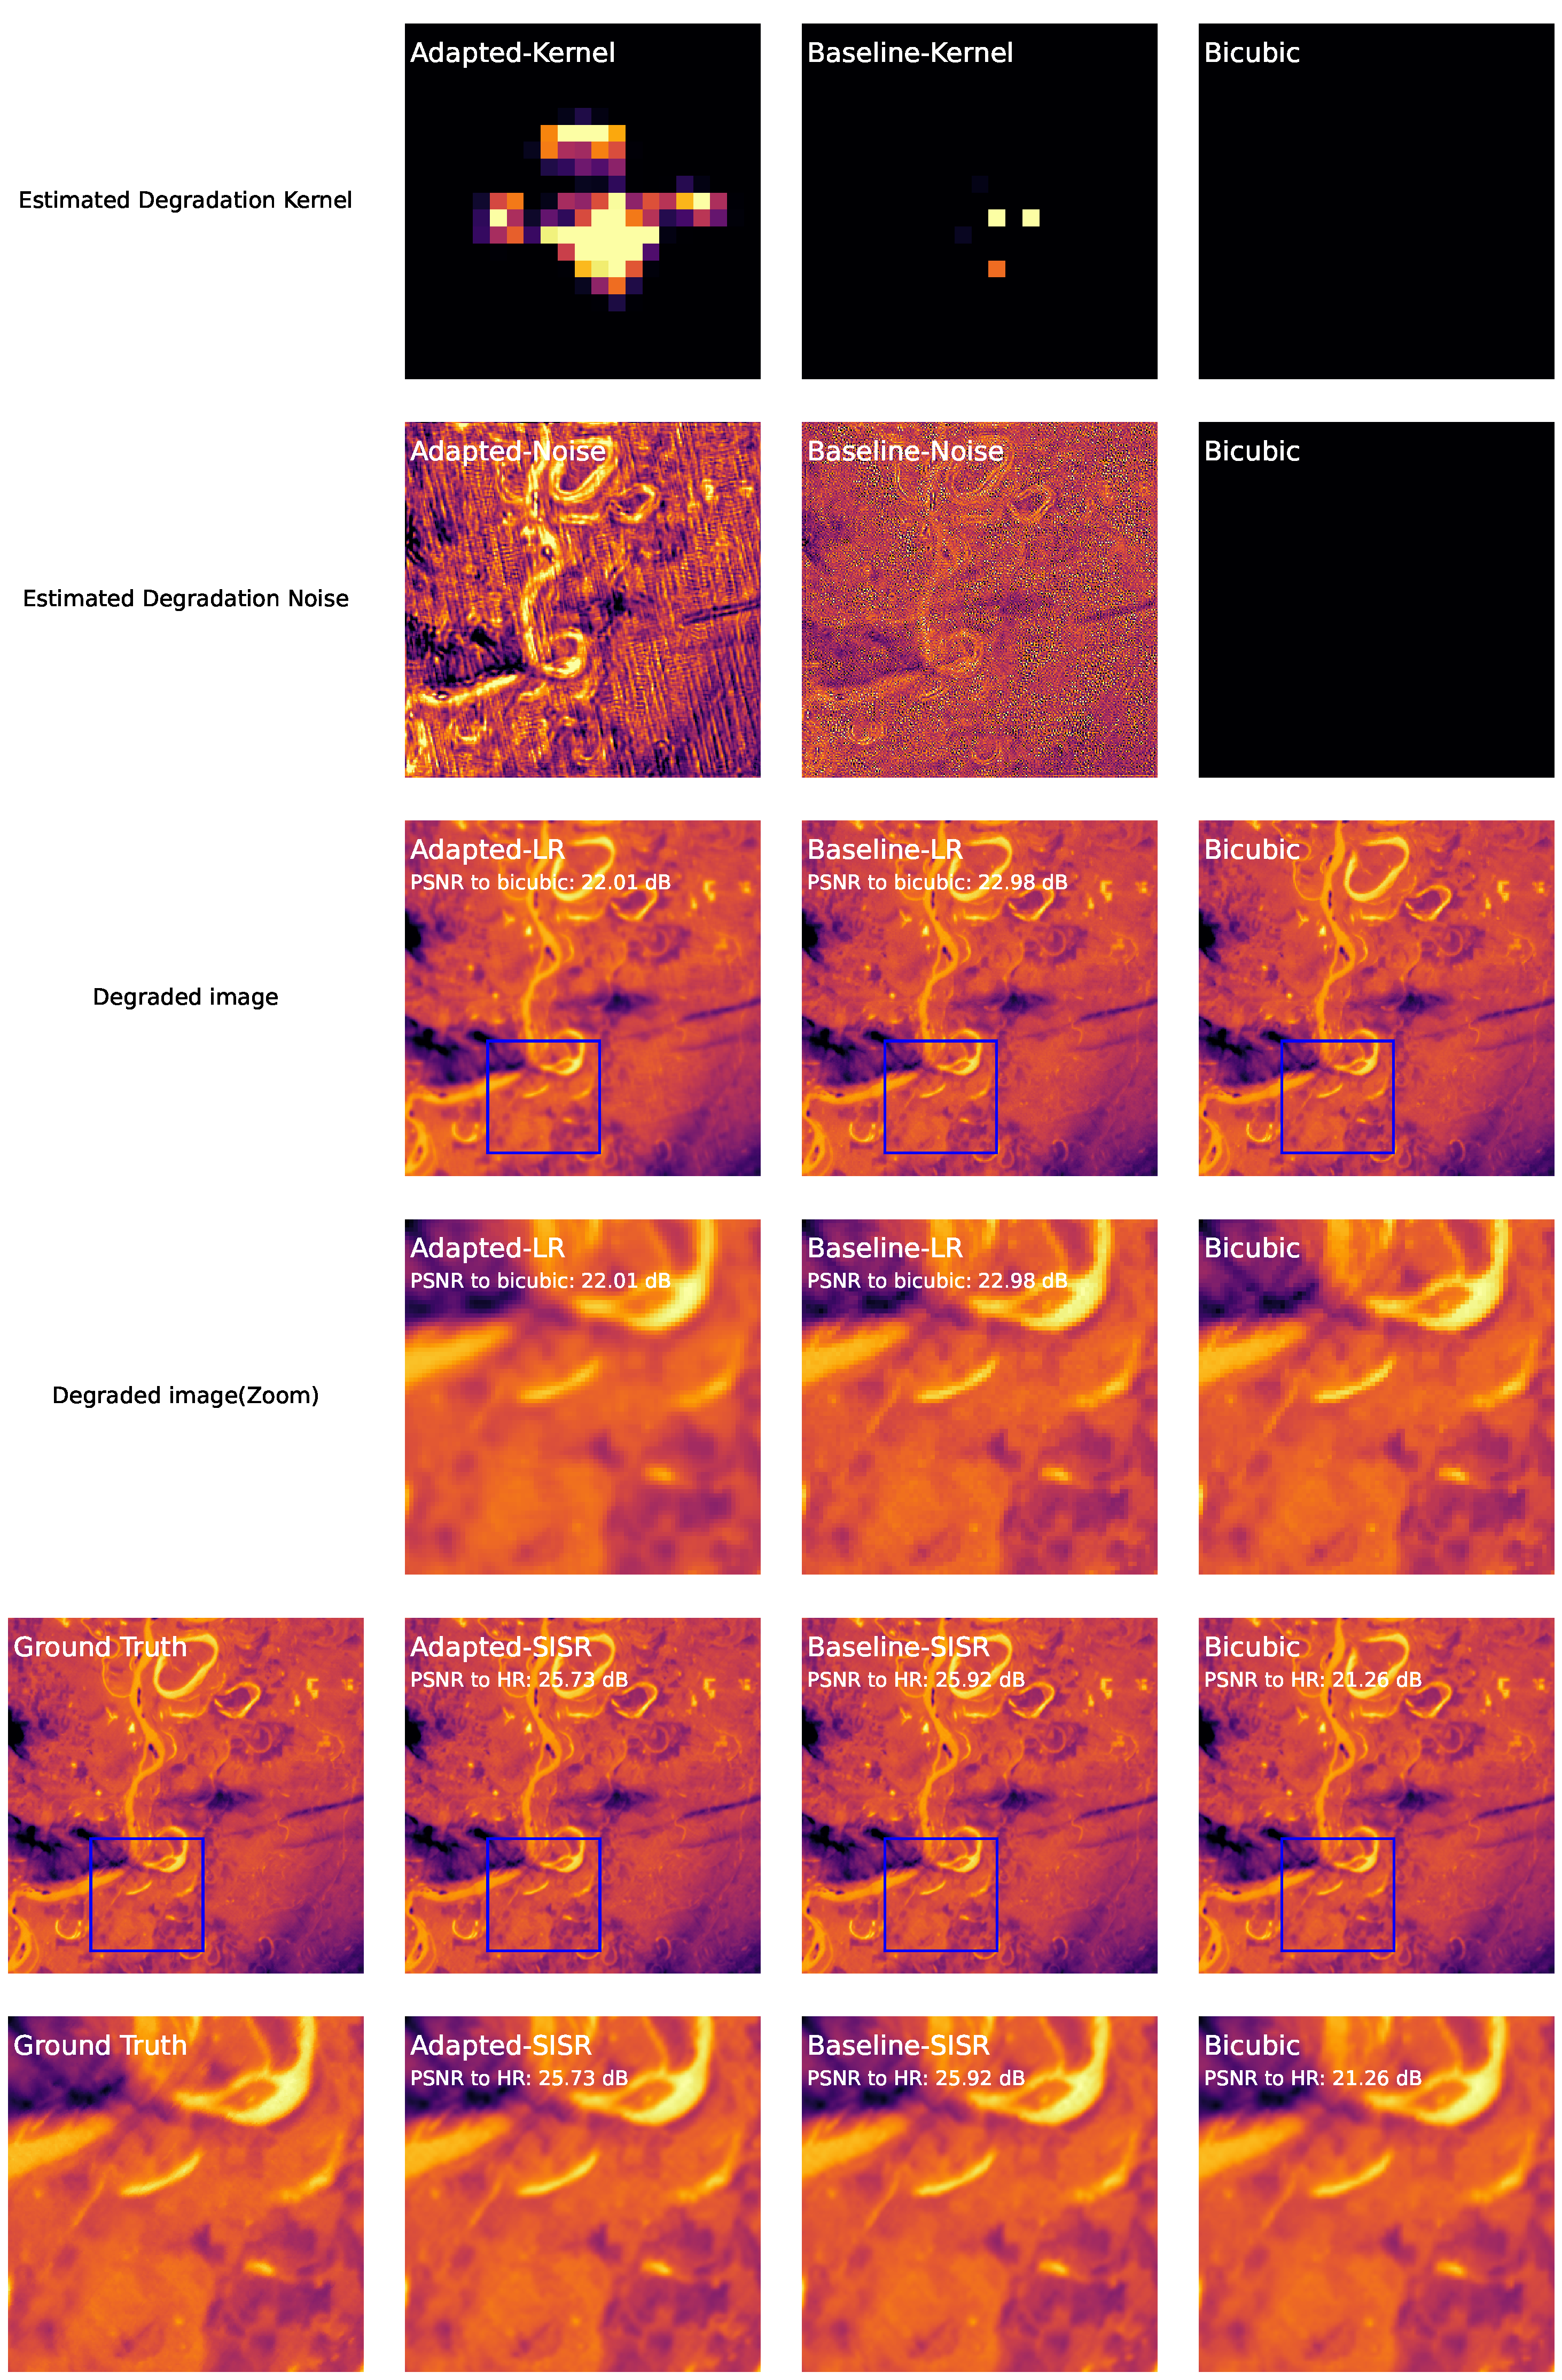
\includegraphics[scale=0.29]{Includes/5-source-prediction-sample.pdf}
            \caption{\small{\small{Applying degradation models on an HR sample. The two upper rows show the estimated kernels and noise for each pipeline (the reference does not perform any estimation). The degraded images from each pipeline are displayed below. The PSNR is calculated against the bicubic downsampling LR. The SR results are displayed in the last two rows. The PSNR for each SR method is calculated against the ground truth.}}
            }
            \label{fig:5-source_domain_sample}
        \end{figure}



        In Fig \ref{fig:5-lr-images-fft.pdf}, the frequency domain of the LR images is analyzed.
        By visual inspection of the FFTs, it is observed that the adapted LR loses more information than the baseline LR as the log magnitude of the FFT diminishes faster and closer to the center.
        The baseline-LR FFT is very close to the Gaussian blurring + bicubic upsampling FFT, suggesting that the baseline pipeline is able to mimic this known degradation model.

        \begin{figure}[H]
            \centering
            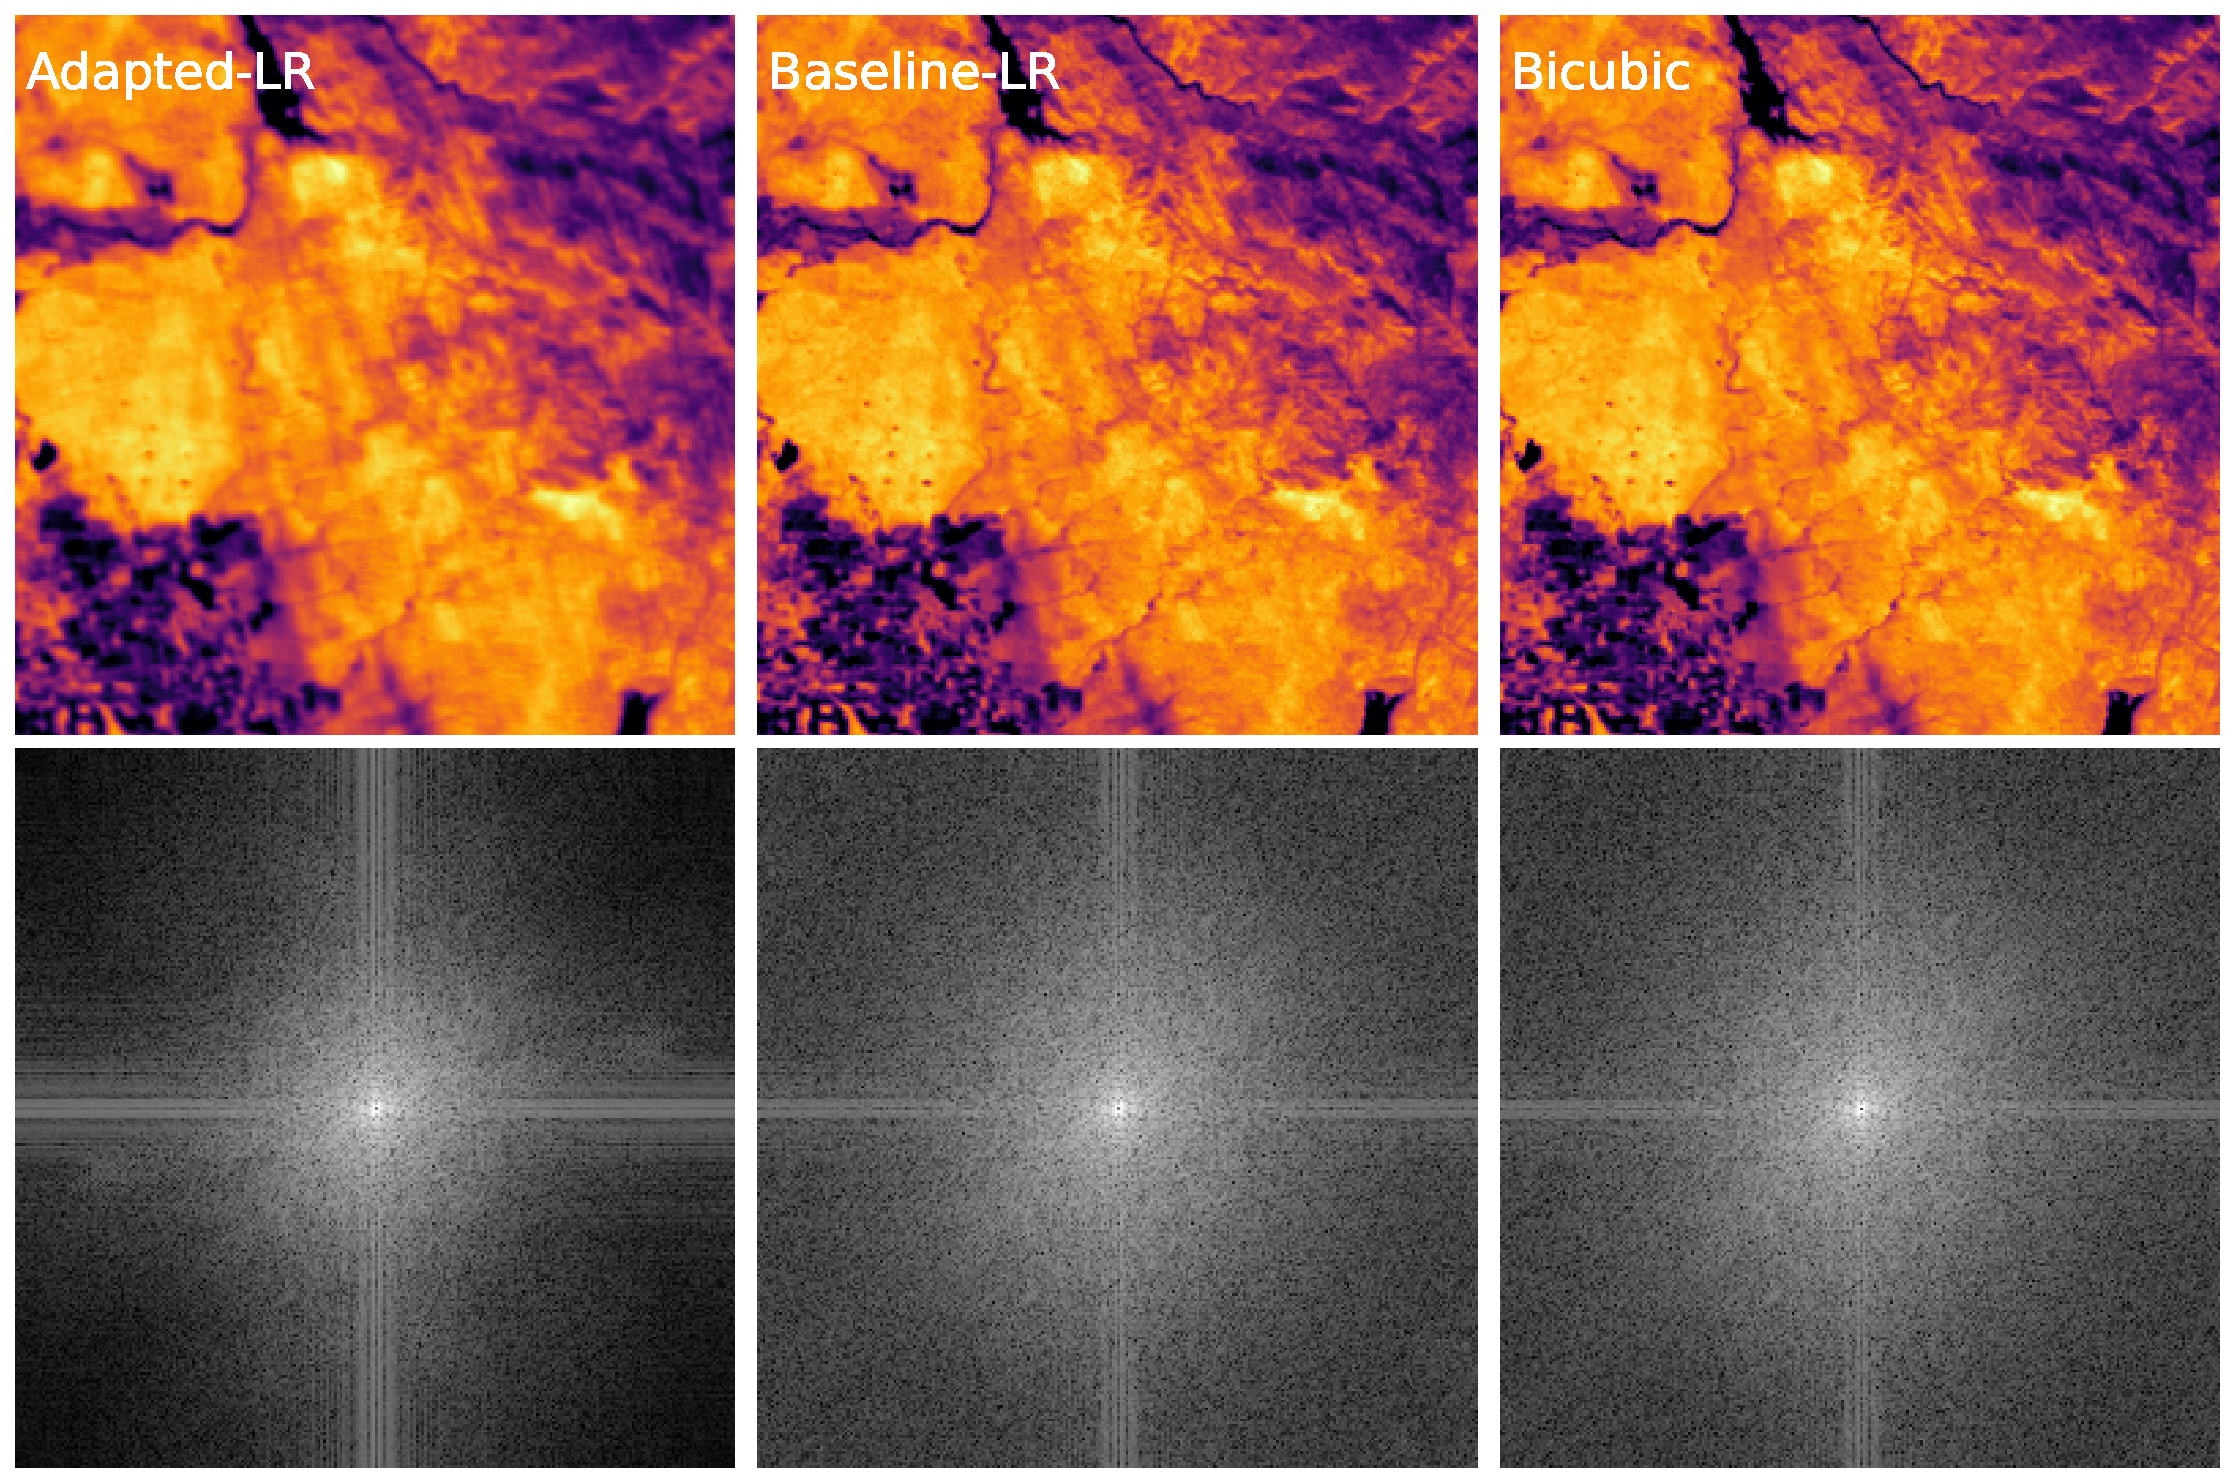
\includegraphics[scale=0.3]{Includes/5-lr-images-fft.pdf}
            \caption{Log magnitude of the FFT for the LR images obtained by the pipelines and the Gaussian blurring + bicubic upsampling.}
            \label{fig:5-lr-images-fft.pdf}
        \end{figure}

        The radial profile of the log magnitude of the FFT for the LR images is shown in Fig. \ref{fig:5-lr-images-fft-comparison.pdf}, confirming what was previously observed . When compared to bicubic downsampling + white noise,
        the adapted degradation model diminishes the high-frequency components more than the baseline. This effect starts at 0.1 cycles per pixel, with a stable attenuation in the order of 6dB from 0.2 to 0.5 cycles per pixel. 
        It is important to note that 0.1 cycles per pixel at a 210m GSD corresponds to a cycle frequency of 2100 $m^{-1}$, 0.2 cycles per pixel corresponds to 1050 $m^{-1}$ and 0.5 cycles per pixel to 420 $m^{-1}$.
        This suggests that the degradation model from the real FOREST-2 images loses more information than the baseline degradation model.
        An analysis of the whole validation dataset will be further discussed to verify that this behavior is consistent across different scenes and conditions.


        \begin{figure}[H]
            \centering
            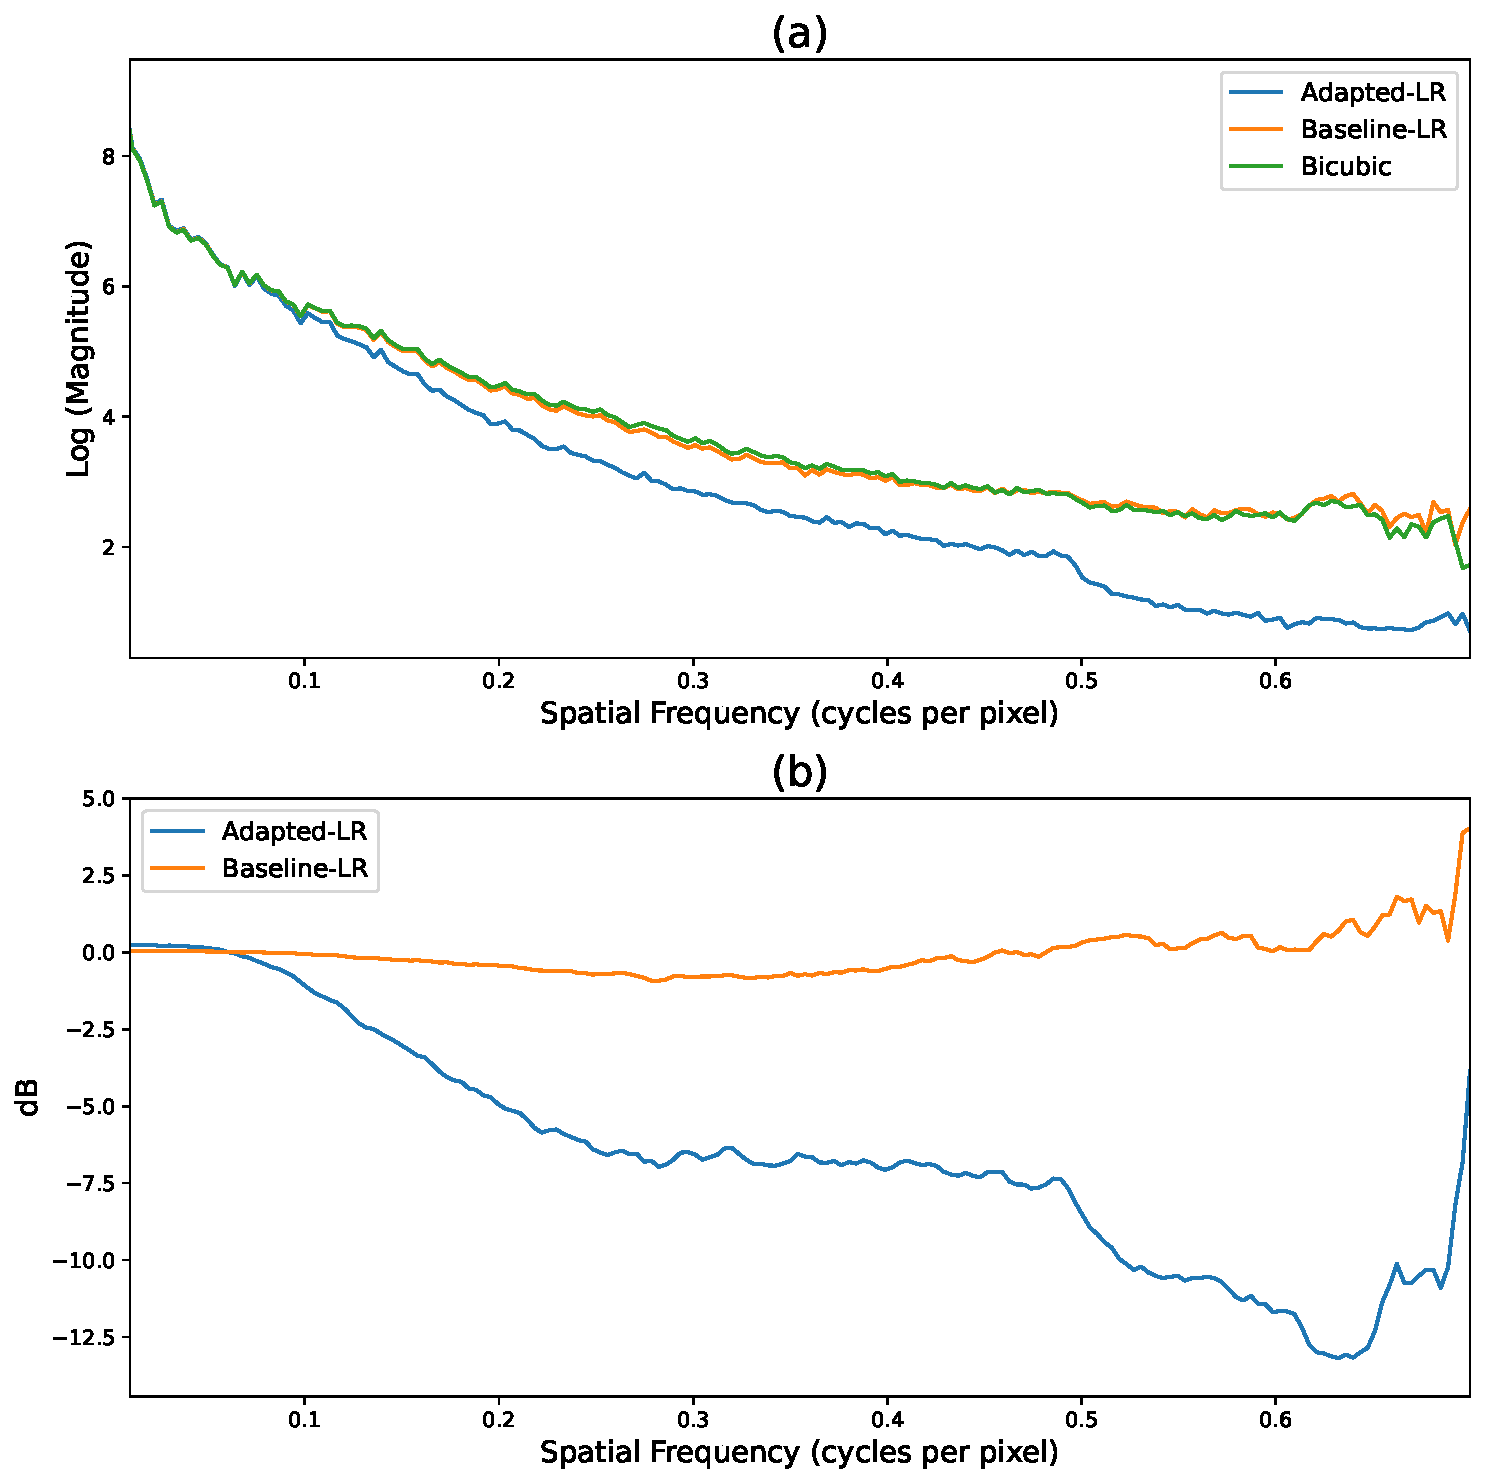
\includegraphics[scale=0.45]{Includes/5-lr-images-fft-comparison.pdf}
            \caption{(a) Radial profile of the log magnitude across the spatial frequency of the LR images obtained by the pipelines and the Gaussian blurring + bicubic downsampling reference. (b) amplification in dB of each pipeline with respect to Gaussian blurring + bicubic downsampling.}
            \label{fig:5-lr-images-fft-comparison.pdf}
        \end{figure}

        When analyzing the super-resolved images versus the ground truth in the frequency domain, a very similar frequency response is observed for both pipelines.
        Moreover, the SR images are able to stay above -3dB, a standard threshold used in the literature, up until 0.2 cycles per pixel, which corresponds to 350$m^{-1}$ when each pixel equals 70m.
        This suggests that the SR model in the adapted pipeline is able to recover the lost information up until those frequencies due to its more complex degradation model.
        Starting at 0.2 cycles per pixel, a decrease in amplification is observed for both pipelines but more steeply for the adapted pipeline.
        This may be related to the fact that the adapted degradation model attenuates higher frequencies even more than the baseline. 
        A limit for the SR PSNR is also noted, even with the baseline, implying that the SR model is not able to recover all details with respect to the HR image.

        \begin{figure}[H]
            \centering
            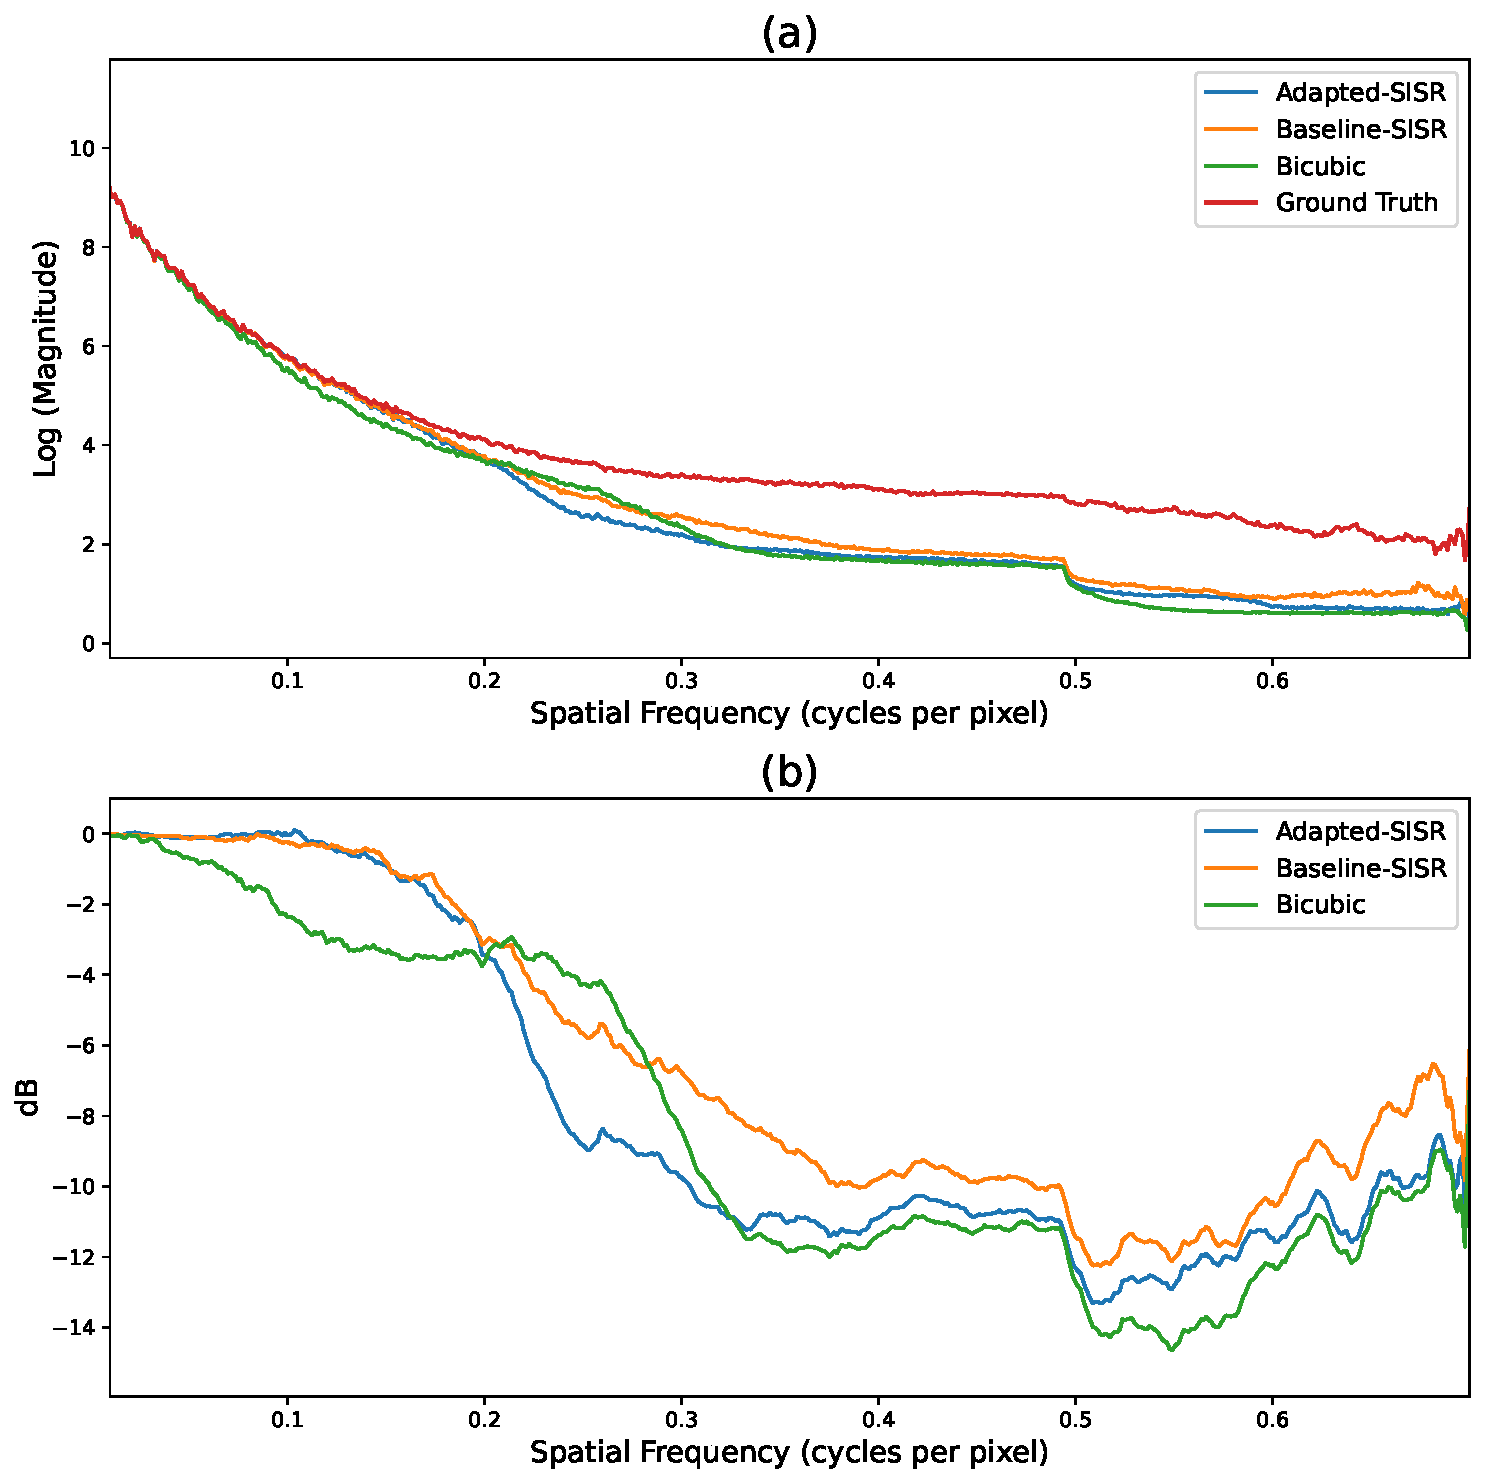
\includegraphics[scale=0.5]{Includes/5-source-sr-fft-comparison.pdf}
            \caption{Frequency domain analysis of the SR images and the ground truth displayed in Fig. \ref{fig:5-source_domain_sample}.
                     In (a), the log of the magnitude of the FFT for the SR images and the ground truth is shown.
                     (b) shows the amplification of each SR image with respect to the ground truth.}
            \label{fig:5-source-sr-fft-comparison}
        \end{figure}

        \subsubsection{Probabilistic degradation models comparison}

        In order to better understand the nature of the kernel generator, its output was extracted 2000 times using different realizations of the random variable $z_k$.
        The pixel-wise mean and standard deviation of the sampled kernels were then computed.
        It is important to note that the experiment configuration assumes that the kernel does not depend on the pixel content or position, resulting in one kernel per image.
        The results are shown in Fig. \ref{fig:5-source-kernel-mean-std}. 
        In order to make the standard deviation of each pixel comparable, its value is normalized by the mean of the corresponding pixel. 
        This allows the expression of the standard deviation as a percentage of the corresponding pixel mean value.
        
        While the baseline and the adapted kernel have the maximum mean and standard deviation in the same pixel, the adapted one denotes a bigger surface.  
        The baseline kernel is composed of a few pixels very close to each other.
        Additionally, the maximum mean in the baseline model is close to 0.7, while the value for the adapted one is close to 0.1.
        This suggests that the adapted kernel is more complex and spread out, while the baseline kernel is simpler and concentrated.
        As a result, the adapted kernel produces blurrier images.
        
        The figure also displays the benefits of the stochastic nature of the degradation model.
        Using only one HR image, the generator is able to produce a wide variety of LR pairs, allowing the training of SR models that may generalize better.

        \begin{figure}[H]
            \centering
            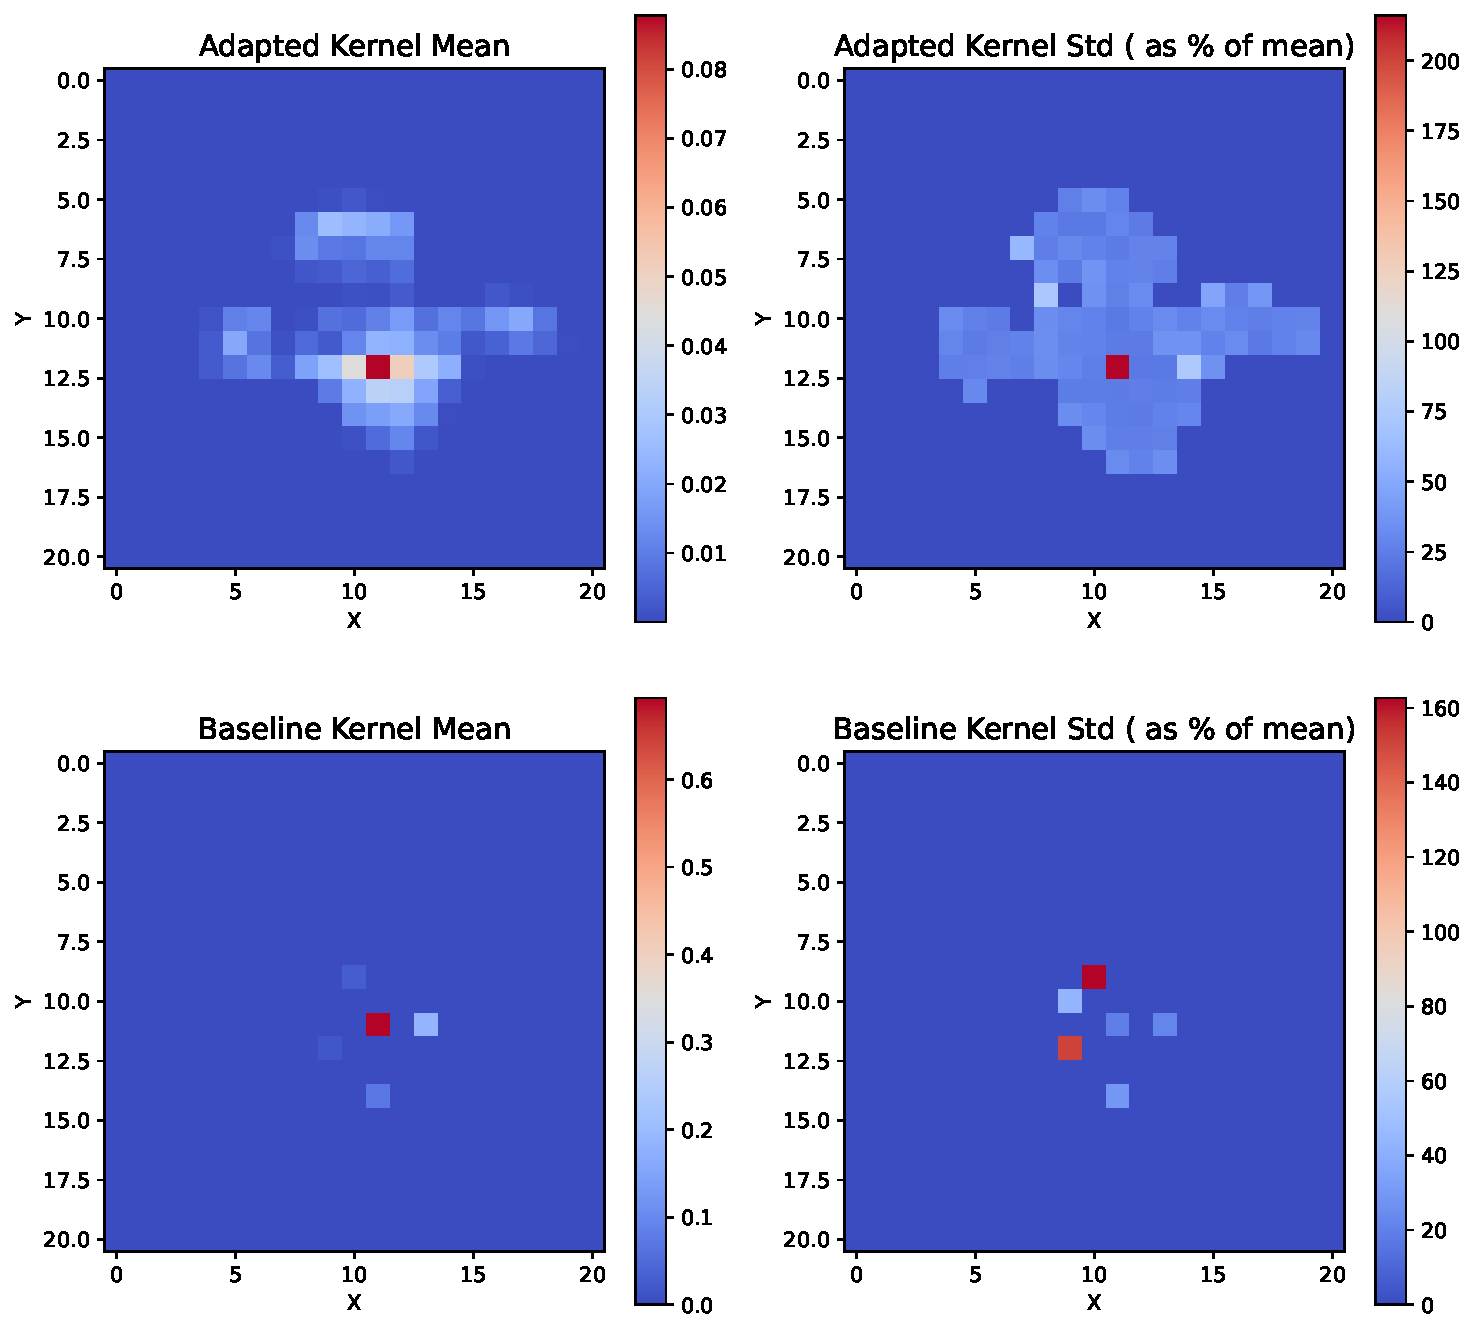
\includegraphics[width=\textwidth]{Includes/5-source-kernel-mean-std.pdf}
            \caption{Mean and standard deviation of the estimated kernels for the baseline and adapted degradation model, using 2000 realizations of $z_k$.
                     The standard deviation of each pixel is normalized by the corresponding mean value. Kernel pixels with mean lower than $10^{-4}$ are considered with 0 standard deviation for clarity in the plot.}
            \label{fig:5-source-kernel-mean-std}
        \end{figure}

        In the case of the noise, the experiment setup assumes that it depends on the pixel content and position.
        For that reason, two different characterizations were done. 
        First, the stochastic component of the noise will be assessed by computing the SNR between the clean image $I^{\text{LR}}_{\text{clean}}$ product of the convolution between $I^{\text{HR}}$ and the kernel, and the output of the noise module, using 2000 different realizations of $z_n$.
        Similar to what happens on the kernel, different noise levels can be added to the same image in order to enrich the dataset even more. It can also be noted that for this particular image, the SNR of the baseline model is higher.

        
        \begin{figure}[H]
            \centering
            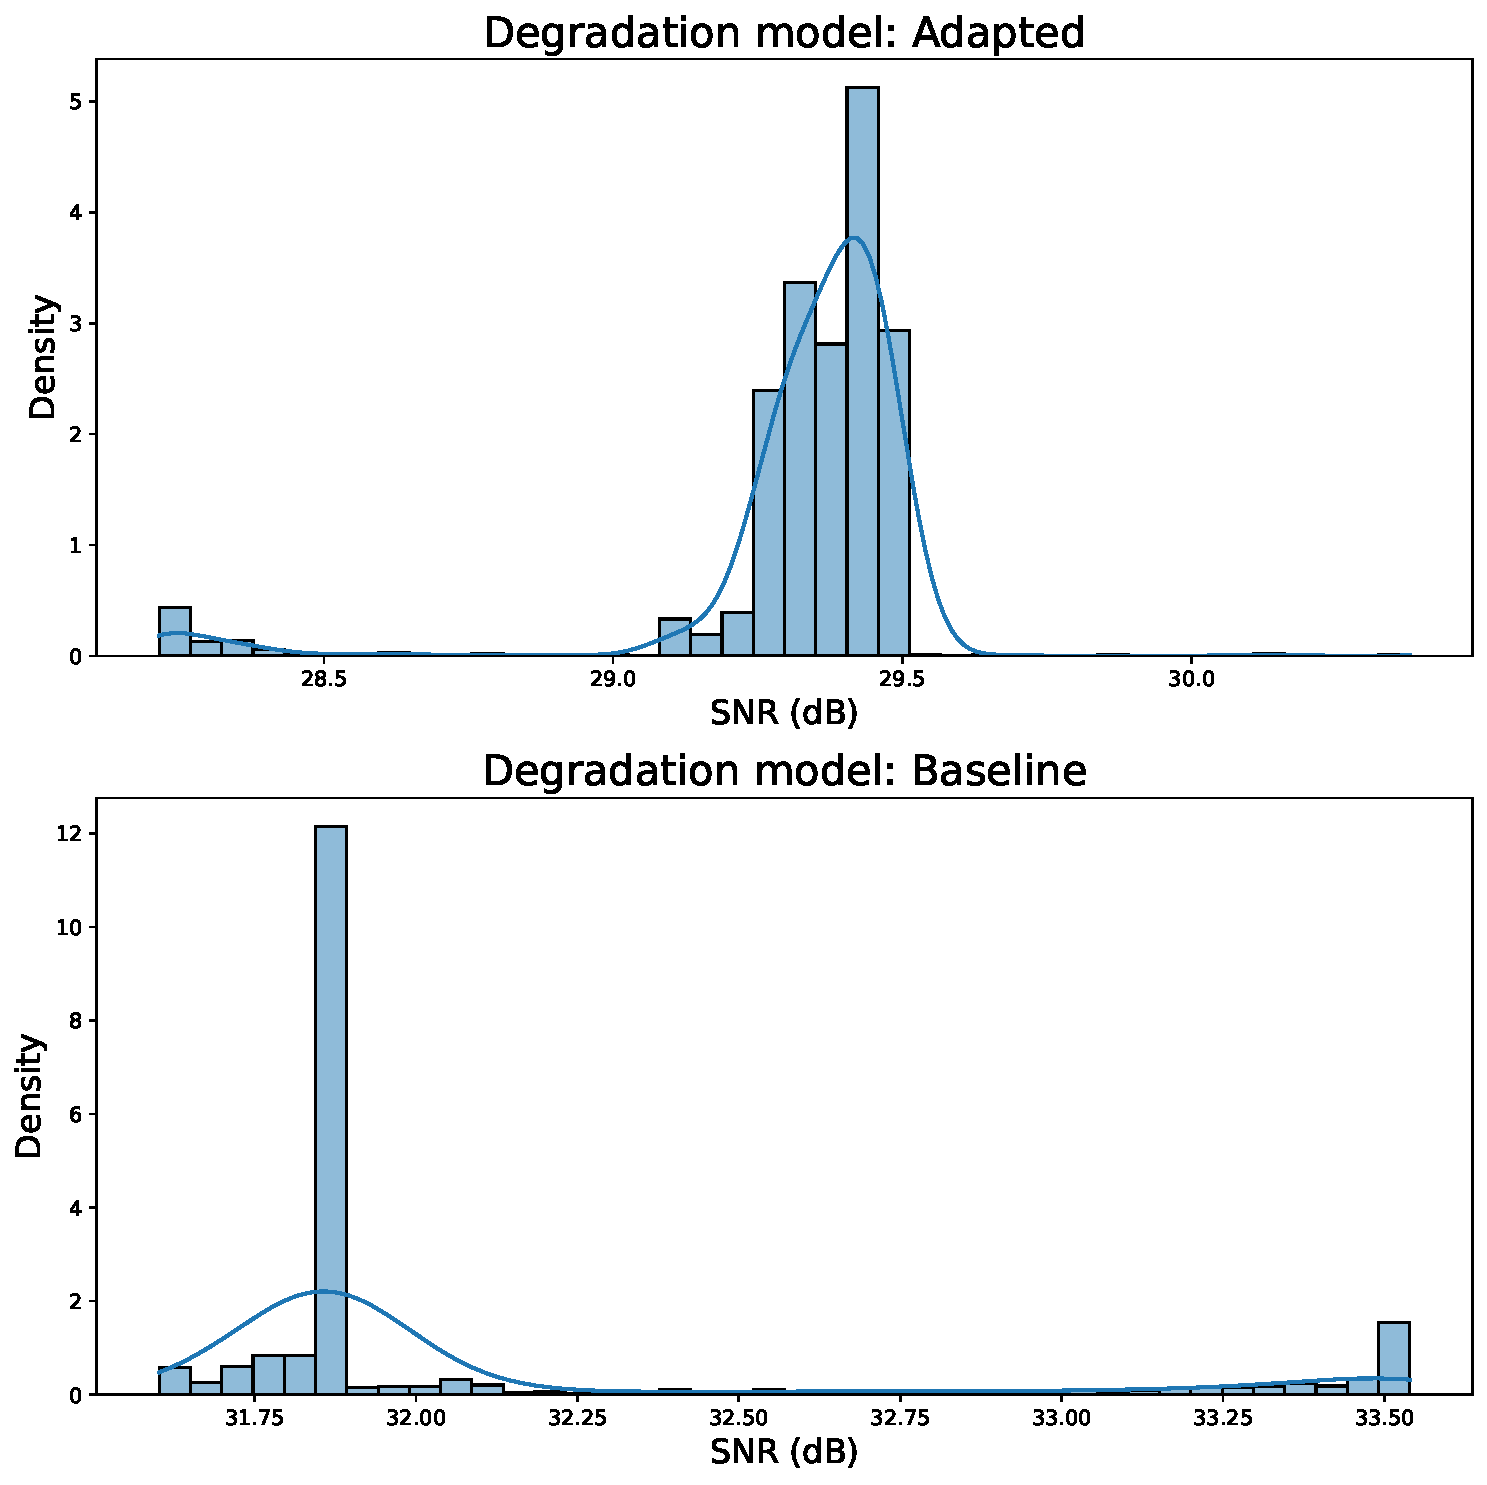
\includegraphics[width=\textwidth]{Includes/5-source-noise-1-sample.pdf}
            \caption{Distribution of SNR values using $I^{\text{LR}}_{\text{clean}}$, product of the convolution of the kernel and $I^{\text{HR}}_{\text{clean}}$, and the noise module output for both pipelines.
                     The output noise is generated 2000 times, using different realizations of the random variable $z_n$ for each iteration and the same input image.
                    }
            \label{fig:5-source-noise-1-sample}
        \end{figure}
        

        Second, and to further analyze the differences between the degradation models, the SNR will be computed for the whole validation dataset.
        An estimated density function of the SNR for each pipeline is shown in Fig. \ref{fig:5-source-noise-SNR}.
        The SNR is, in general, bigger when using the baseline model compared to the adapted one.
        This implies that in the output of the adapted model generator, the noise tends to have more power. 

        \begin{figure}[H]
            \centering
            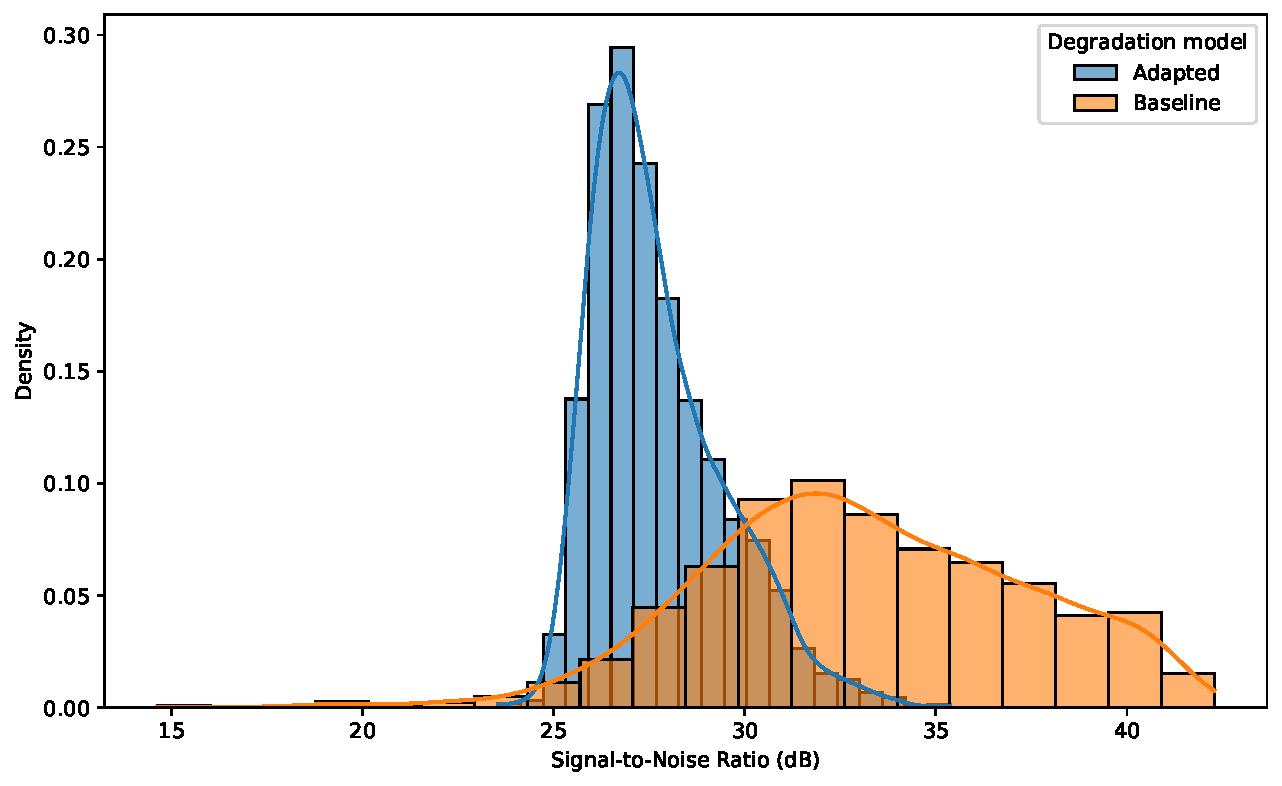
\includegraphics[width=\textwidth]{Includes/5-source-noise-SNR.pdf}
            \caption{Comparison of the SNR expressed in dB of the LR images generated by the baseline and adapted degradation model.}
            \label{fig:5-source-noise-SNR}
        \end{figure}


        A similar procedure is performed but calculating the Pearson correlation coefficient between the input image $I^{\text{LR}}_{\text{clean}}$ and the output of the noise module. The adapted degradation model produces noise highly correlated with the input.


        \begin{figure}[H]
            \centering
            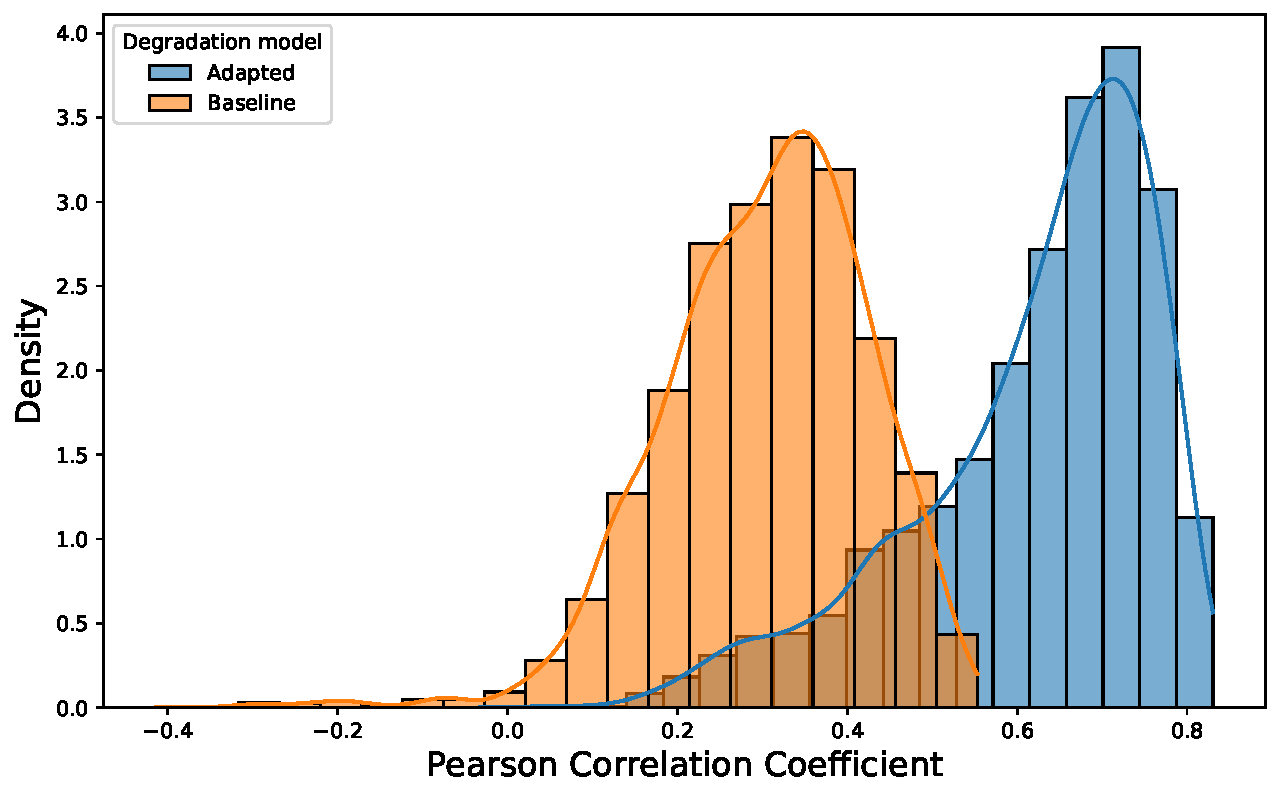
\includegraphics[width=\textwidth]{Includes/5-source-noise-correlation.pdf}
            \caption{Comparison of the Pearson correlation coefficient between $I^{\text{LR}}_{\text{clean}}$ and the output of the noise module for the baseline and adapted degradation model.}
            \label{fig:5-source-noise-correlation}
        \end{figure}

        

        The observed effects support what is observed in Fig. \ref{fig:5-source-domain-comparison}. 
        The adapted pipeline produces broader kernels and noise with more energy that is highly correlated with the image content compared to the baseline pipeline.
        This leads to blurrier and noisier generated LR images. 
        The kernel imposes a low pass filter for the frequency components in the image, and the noise degrades the amount of recoverable signal from it.
        Both components constitute a more challenging scenario for the SR model. 

        \subsubsection{Low resolution images comparison} \label{subsec:results-lr-comparison}

        A quantitative analysis of the LR images yielded by the generator of each pipeline is performed. 
        Fig. \ref{fig:5-source-domain-lr-performance-scatterplot} shows three supervised performance metrics obtained by comparing the LR images with the bicubic downsampling + white noise reference.
        In this case, a consistently higher PSNR and SSIM means that the baseline-LR image is closer to bicubic downsampling + white noise than the one generated by the adapted pipeline. 
        A lower LPIPS means that even using perceptual metrics, the baseline-LR image is also closer.
        This is consistent with the results shown in Fig. \ref{fig:5-source_domain_sample}, where the adapted LR image is more blurry and noisy, suggesting that the unknown degradation is far from the baseline degradation model.
        
        \begin{figure}[H]
            \centering
            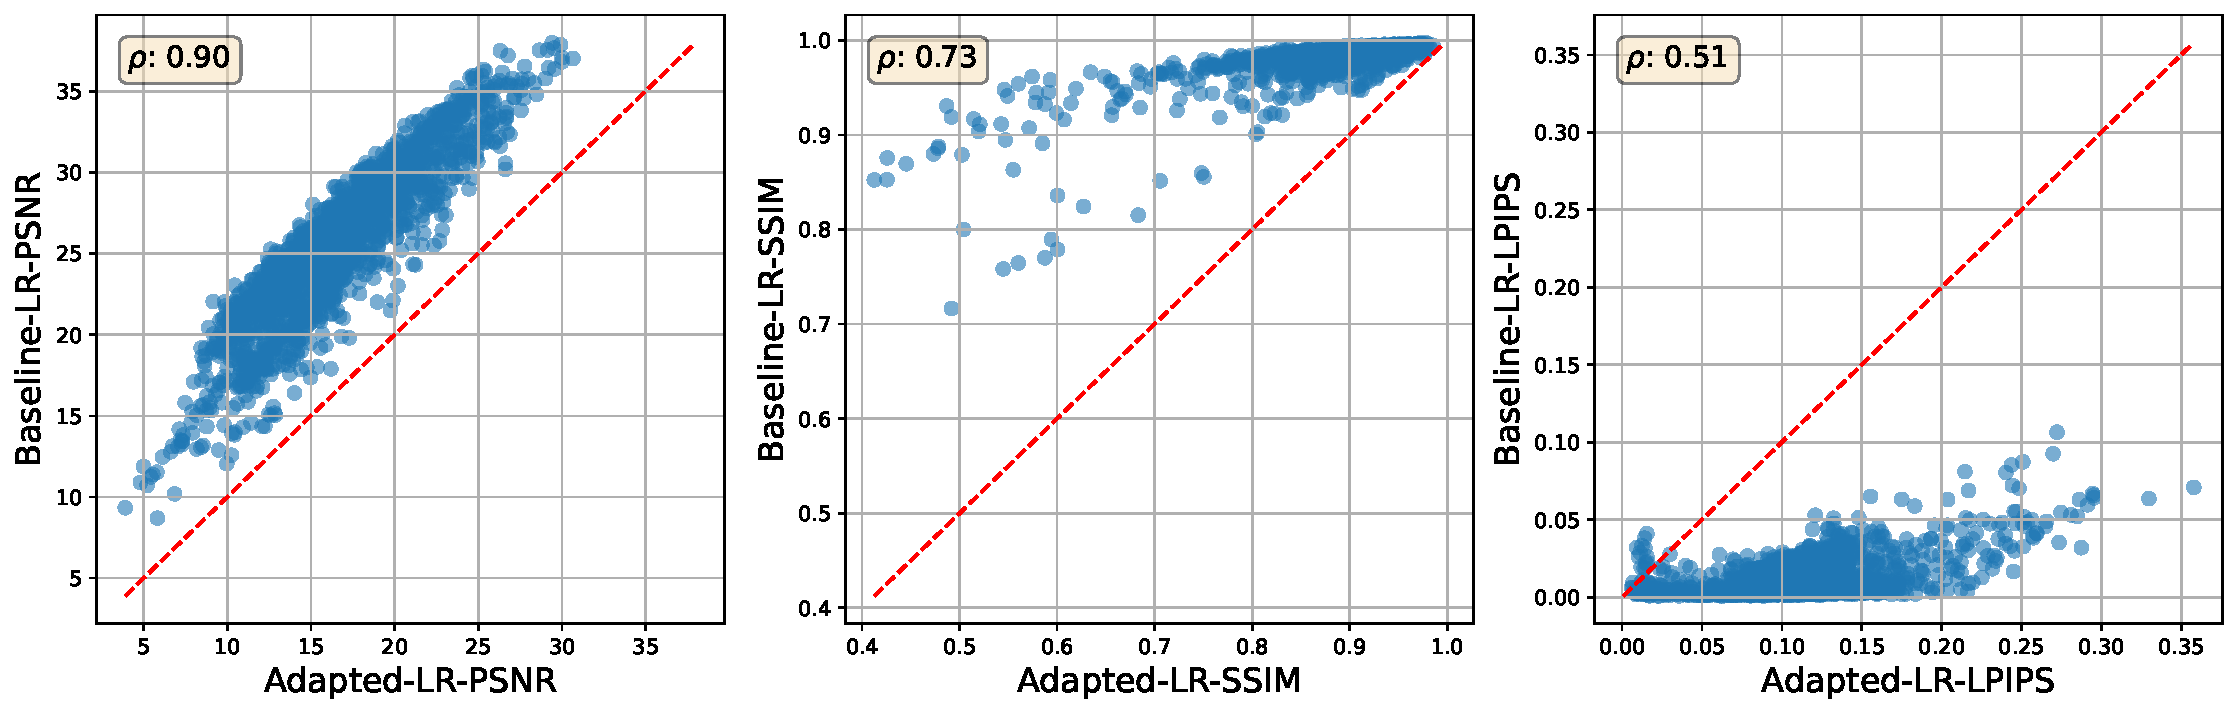
\includegraphics[width=\textwidth]{Includes/5-source-domain-lr-performance-scatterplot.pdf}
            \caption{Performance metrics between the LR images obtained by the pipelines vs the Gaussian blurring + bicubic downsampling degradation.
                     The PSNR is displayed on the left. SSIM and LPIPS are represented in the middle and the right, respectively.}
            \label{fig:5-source-domain-lr-performance-scatterplot}
        \end{figure}




        An alternative way to evaluate the differences in the degradations is by analyzing the frequency domain of the LR images.
        An analysis of the whole validation dataset is performed by calculating the FFT of each LR image and comparing them with the bicubic downsampling + white noise degradation model.
        The results are displayed in Fig. \ref{fig:5-lr-images-fft-comparison} and show that the LR images generated by the adapted pipeline yield a reduction in all frequency components consistently across all samples, with a ± 1 standard deviation interval between -4 and -8 dB from between 0.25 and 0.5 cycles per 210m pixel.

        \begin{figure}[H]
            \centering
            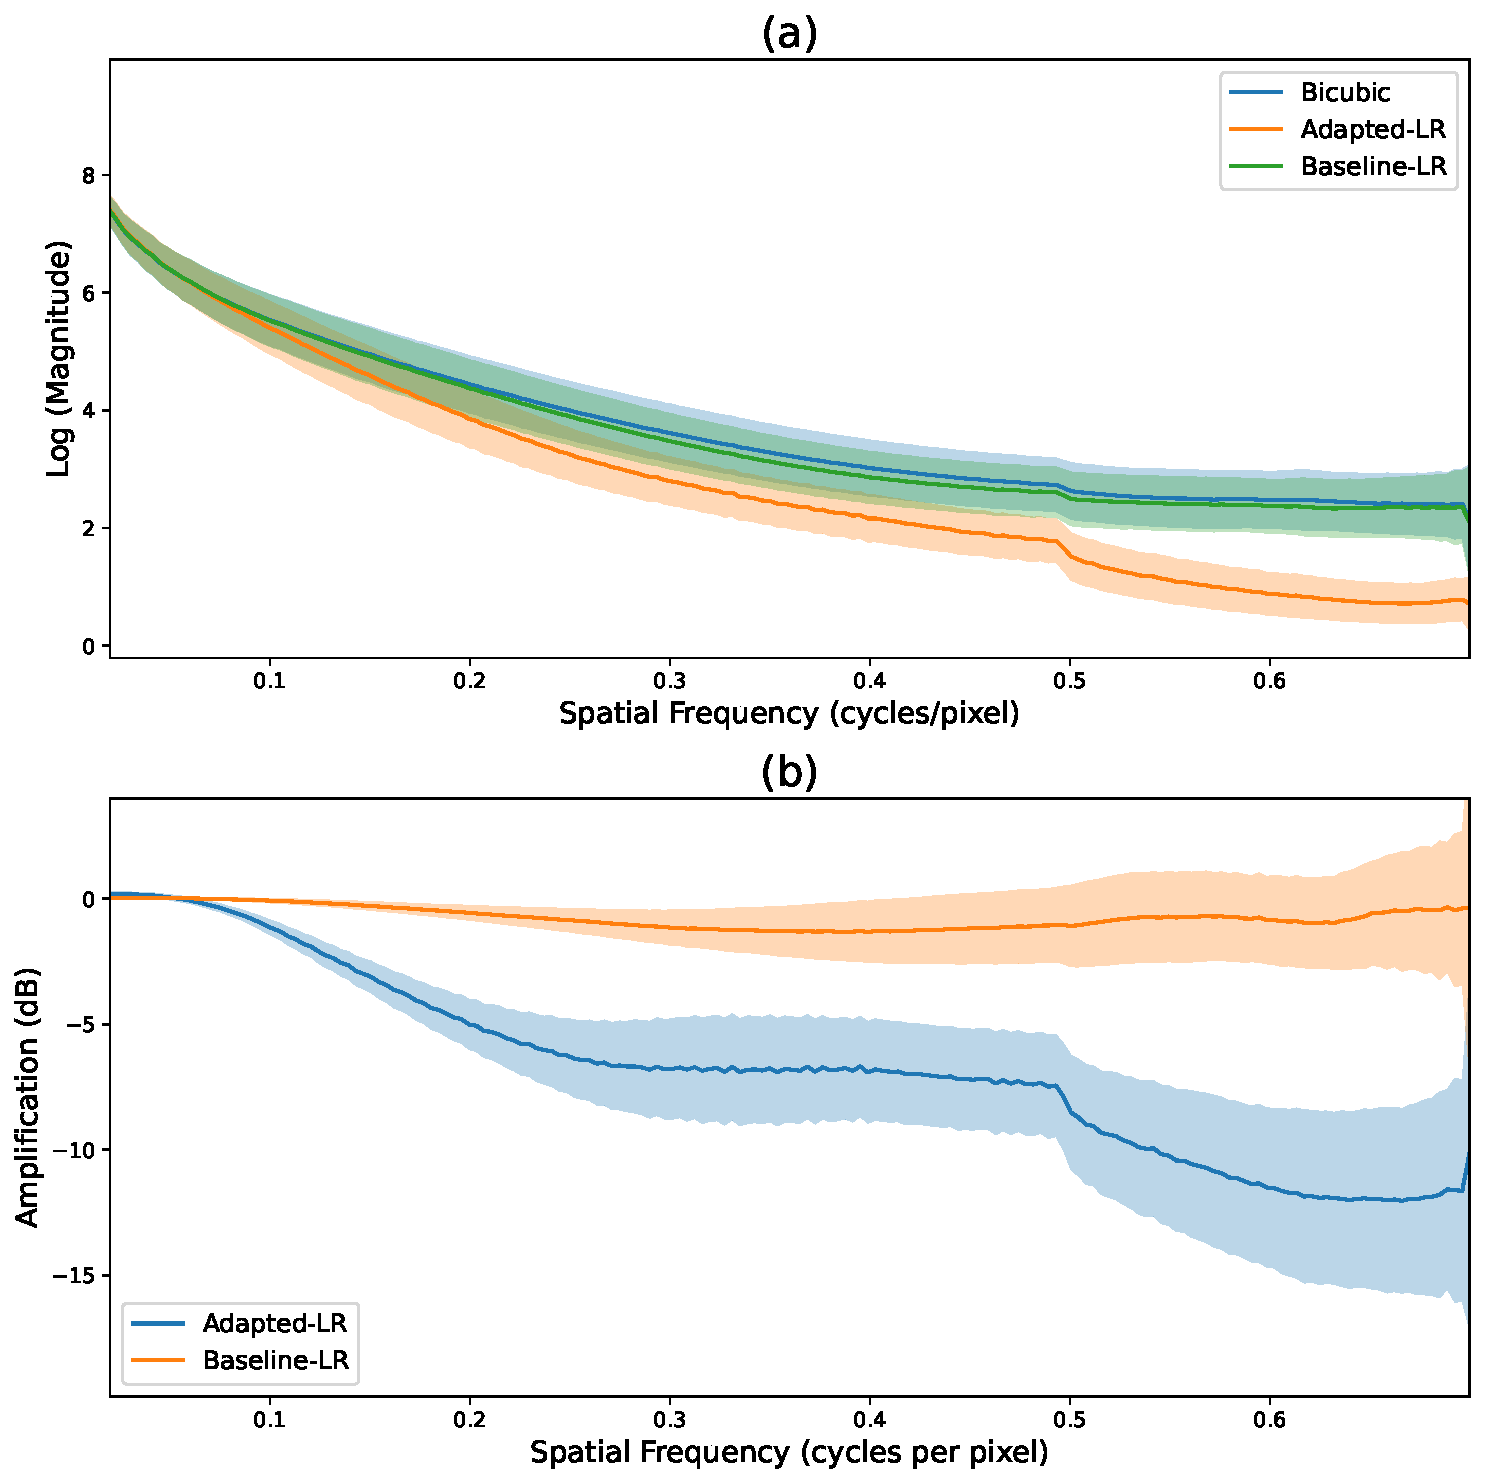
\includegraphics[scale=0.5]{Includes/5-source-lr-amplification-statistics.pdf}
            \caption{Frequency domain analysis of the LR images obtained by applying different degradation models on the HR sample displayed in Fig. \ref{fig:5-source_domain_sample}.
                     In (a), the log of the magnitude of the FFT for the LR images is shown,
                     while in (b), the amplification with respect to a  simple Gaussian blurring + downscaling is shown.
                     The painted area represents the ±1 standard deviation interval}
            \label{fig:5-lr-images-fft-comparison}
        \end{figure}




        \subsubsection{Effects of the degradation model in super resolution performance}

        Another subject of interest is how the degradation model affects the performance of the super resolution process.
        Fig. \ref{fig:5-source-domain-comparison} shows the performance obtained by super resolving the output of each pipeline generator for the whole validation dataset.
        In (a), the corresponding SR model of each pipeline is used to obtain the super-resolved images. 
        The performance in PSNR, SSIM, and LPIPS is very similar.
        In (b), the SR model is discarded, and bicubic upsampling is used to super resolve the degraded images of each pipeline. 
        In this case, using the baseline LR as input consistently yields better results than the adapted LR  in all metrics.
        This suggests that the learned degradation model from FOREST-2 images loses more information than the baseline, resulting in a lower effective ground sampling distance than what was specified in the FOREST-2 fact sheet.
        Consistent with what was found in Figs. \ref{fig:5-source_domain_sample} and \ref{fig:5-source-sr-fft-comparison}, the SR model is able to recover the lost information, as the performance is very similar when employing the SR models. 
        
        \begin{figure}[H]
            \centering
            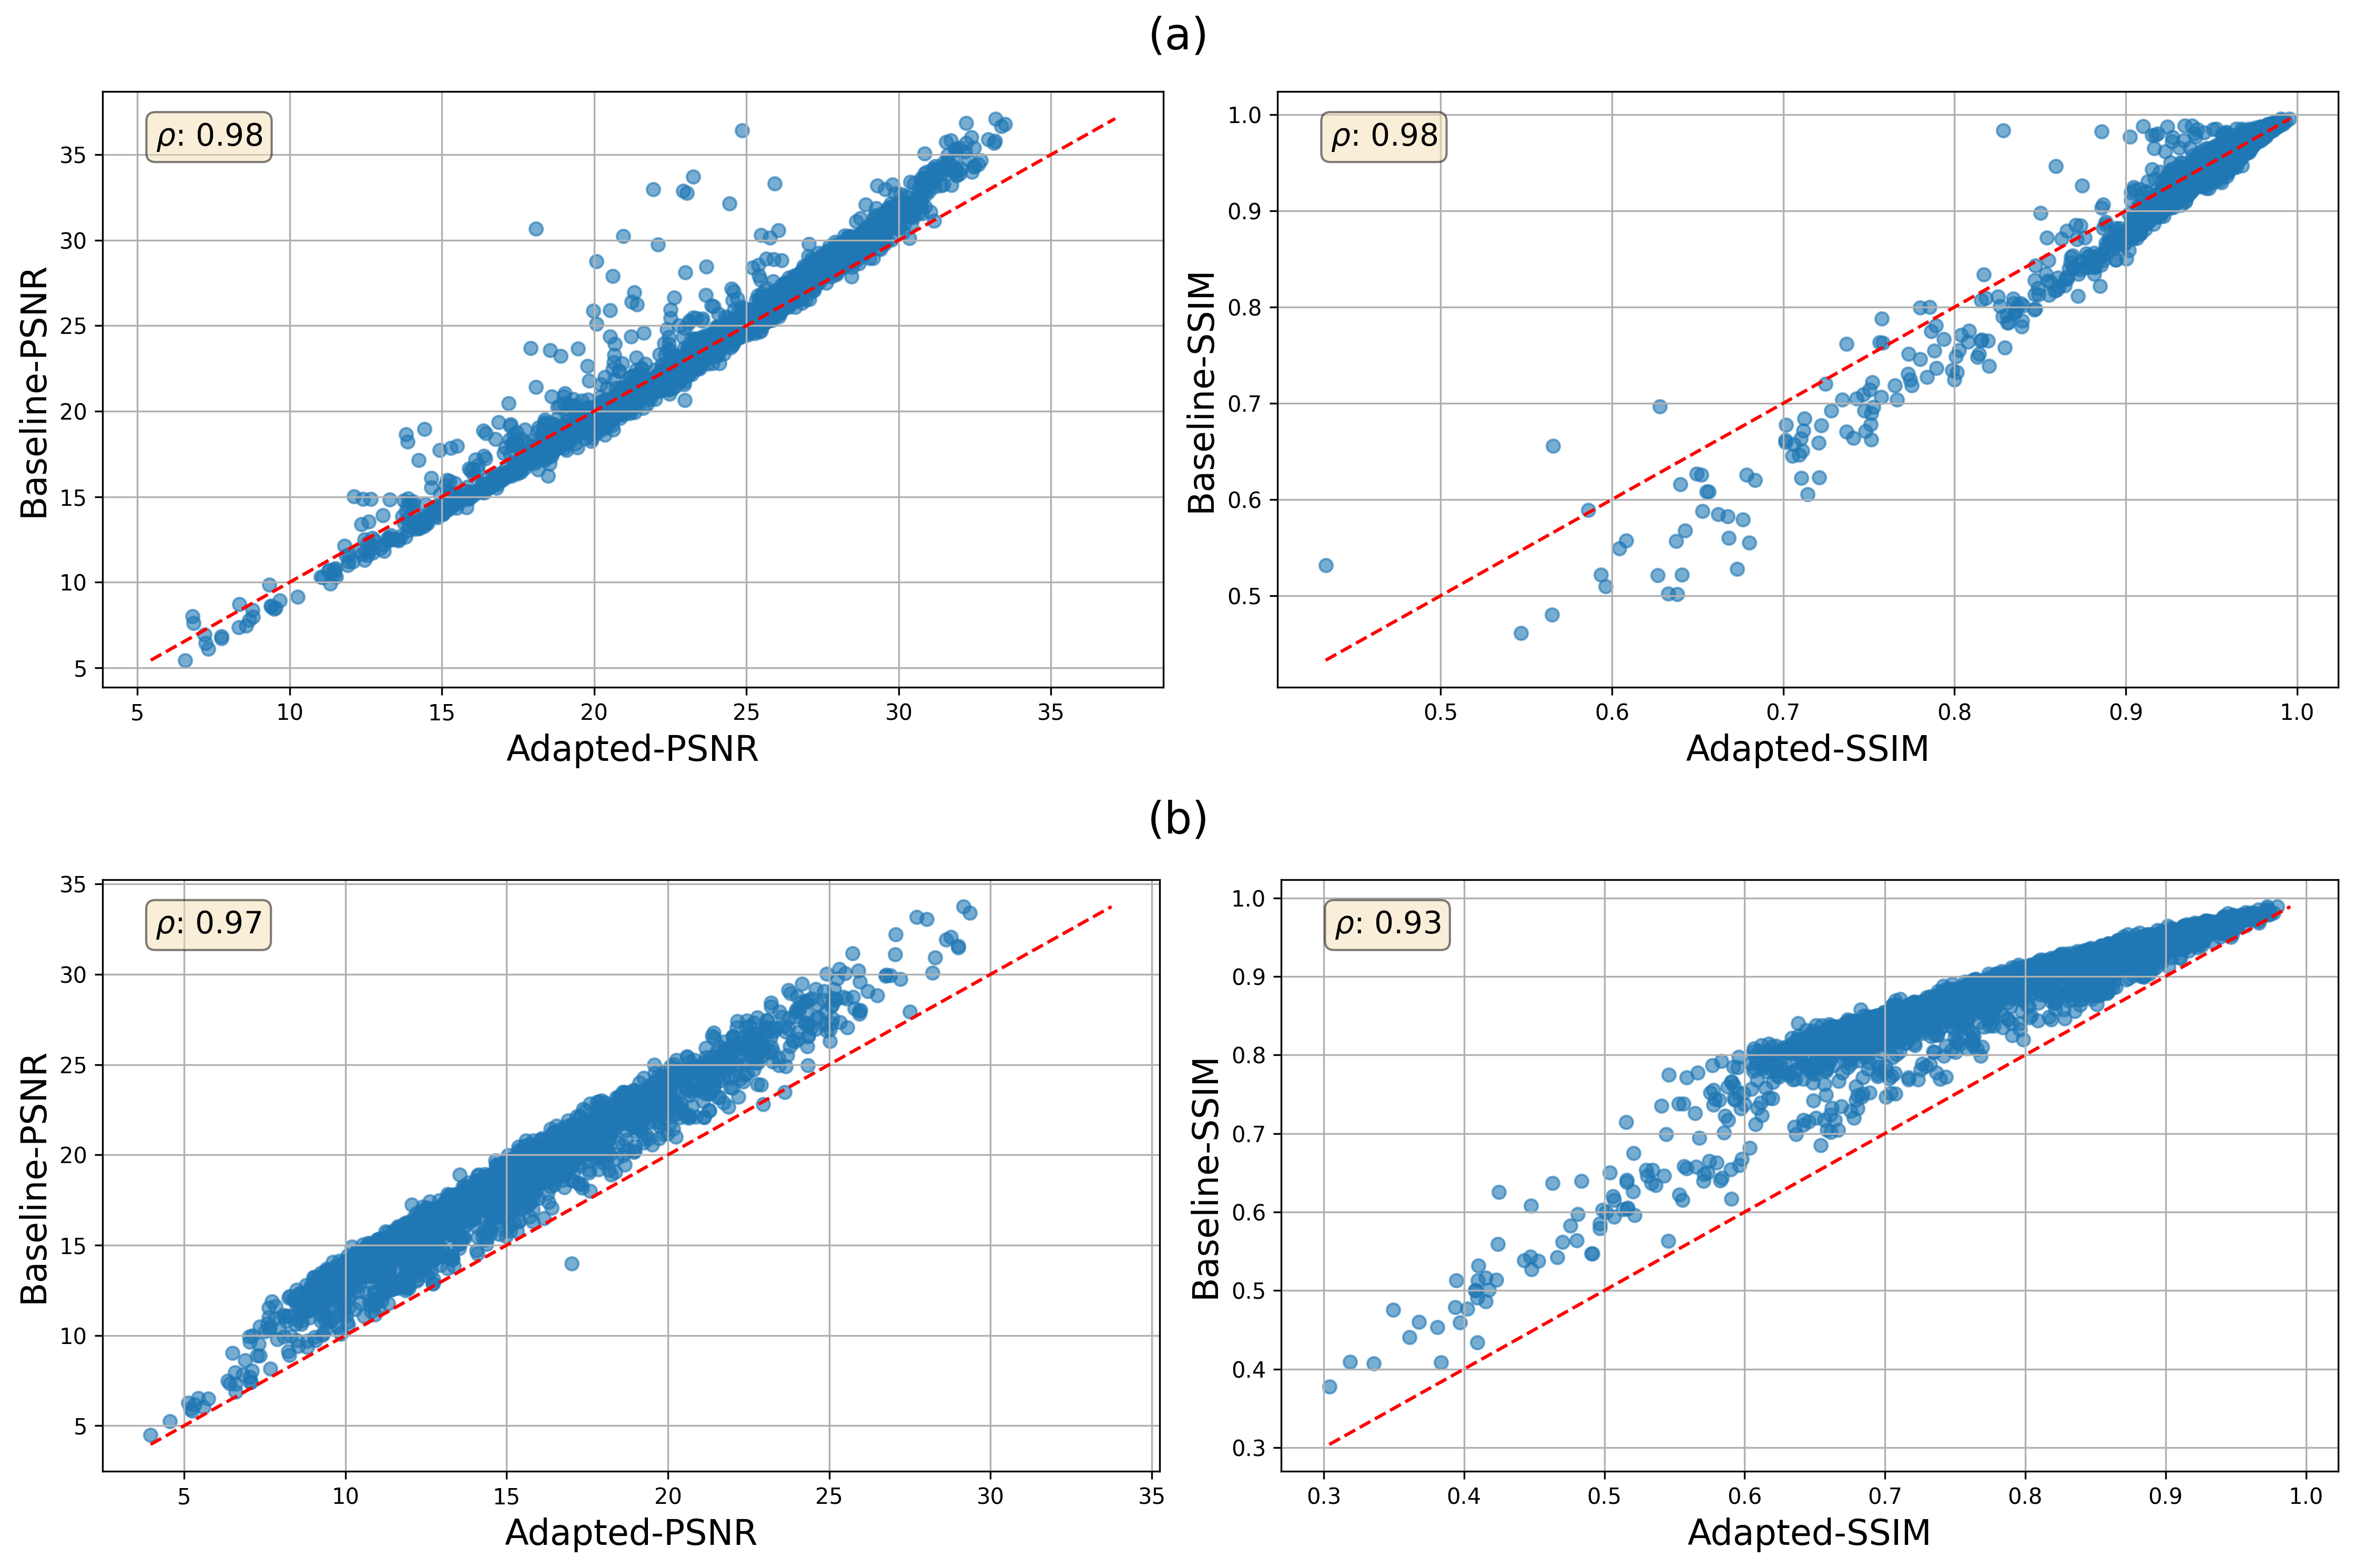
\includegraphics[width=\textwidth]{Includes/5-source-domain-comparison.png}
            \caption{Performance obtained by super resolving the degraded images coming out of the generator. 
                     In (a), the corresponding SR model of each pipeline is used. 
                     In (b), bicubic upsampling is used to super resolve the degraded images instead of the SR model. The Pearson correlation coefficient is represented by $\rho$. }
            \label{fig:5-source-domain-comparison}
        \end{figure}

        Fig \ref{fig:5-source-domain-comparison} proves the relevance of the domain gap in super resolution. The SR model is able to estimate the inverse of the degradation function if given the correct data. The problem relies on the fact that in most experiments, the wrong degradation is shown to the model, forcing it to learn the inverse of an incorrect function.  
        This plays an essential role when applying super resolution models to accurate data, where the degradation model may not be known. 

    \subsection{Target domain}

        This subsection will show the results from the experiments performed on the target domain, which is the equivalent of the red arrow flow described in Fig. \ref{fig:3-GAN-degradation-model}.
        In this case, the GAN trained for the degradation model is discarded, and only the SR model is used with authentic FOREST-2 images as input.
        Due to the unpaired nature of the dataset, the performance of the SR model can not be evaluated using metrics like PSNR and SSIM. 
        Other alternatives will be presented, and a qualitative analysis will be performed. 
        
        In Fig. \ref{fig:5-target_prediction_sample}, the super resolution models were used with a 264x264 crop of a real FOREST-2 image as an input.
        The results show that the baseline model has very similar results to bicubic upsampling.
        The adapted model, trained using real FOREST-2 images as the target domain, produces sharper images without clearly increasing the overall noise.
        
        


        \begin{figure}[H]
            \centering
            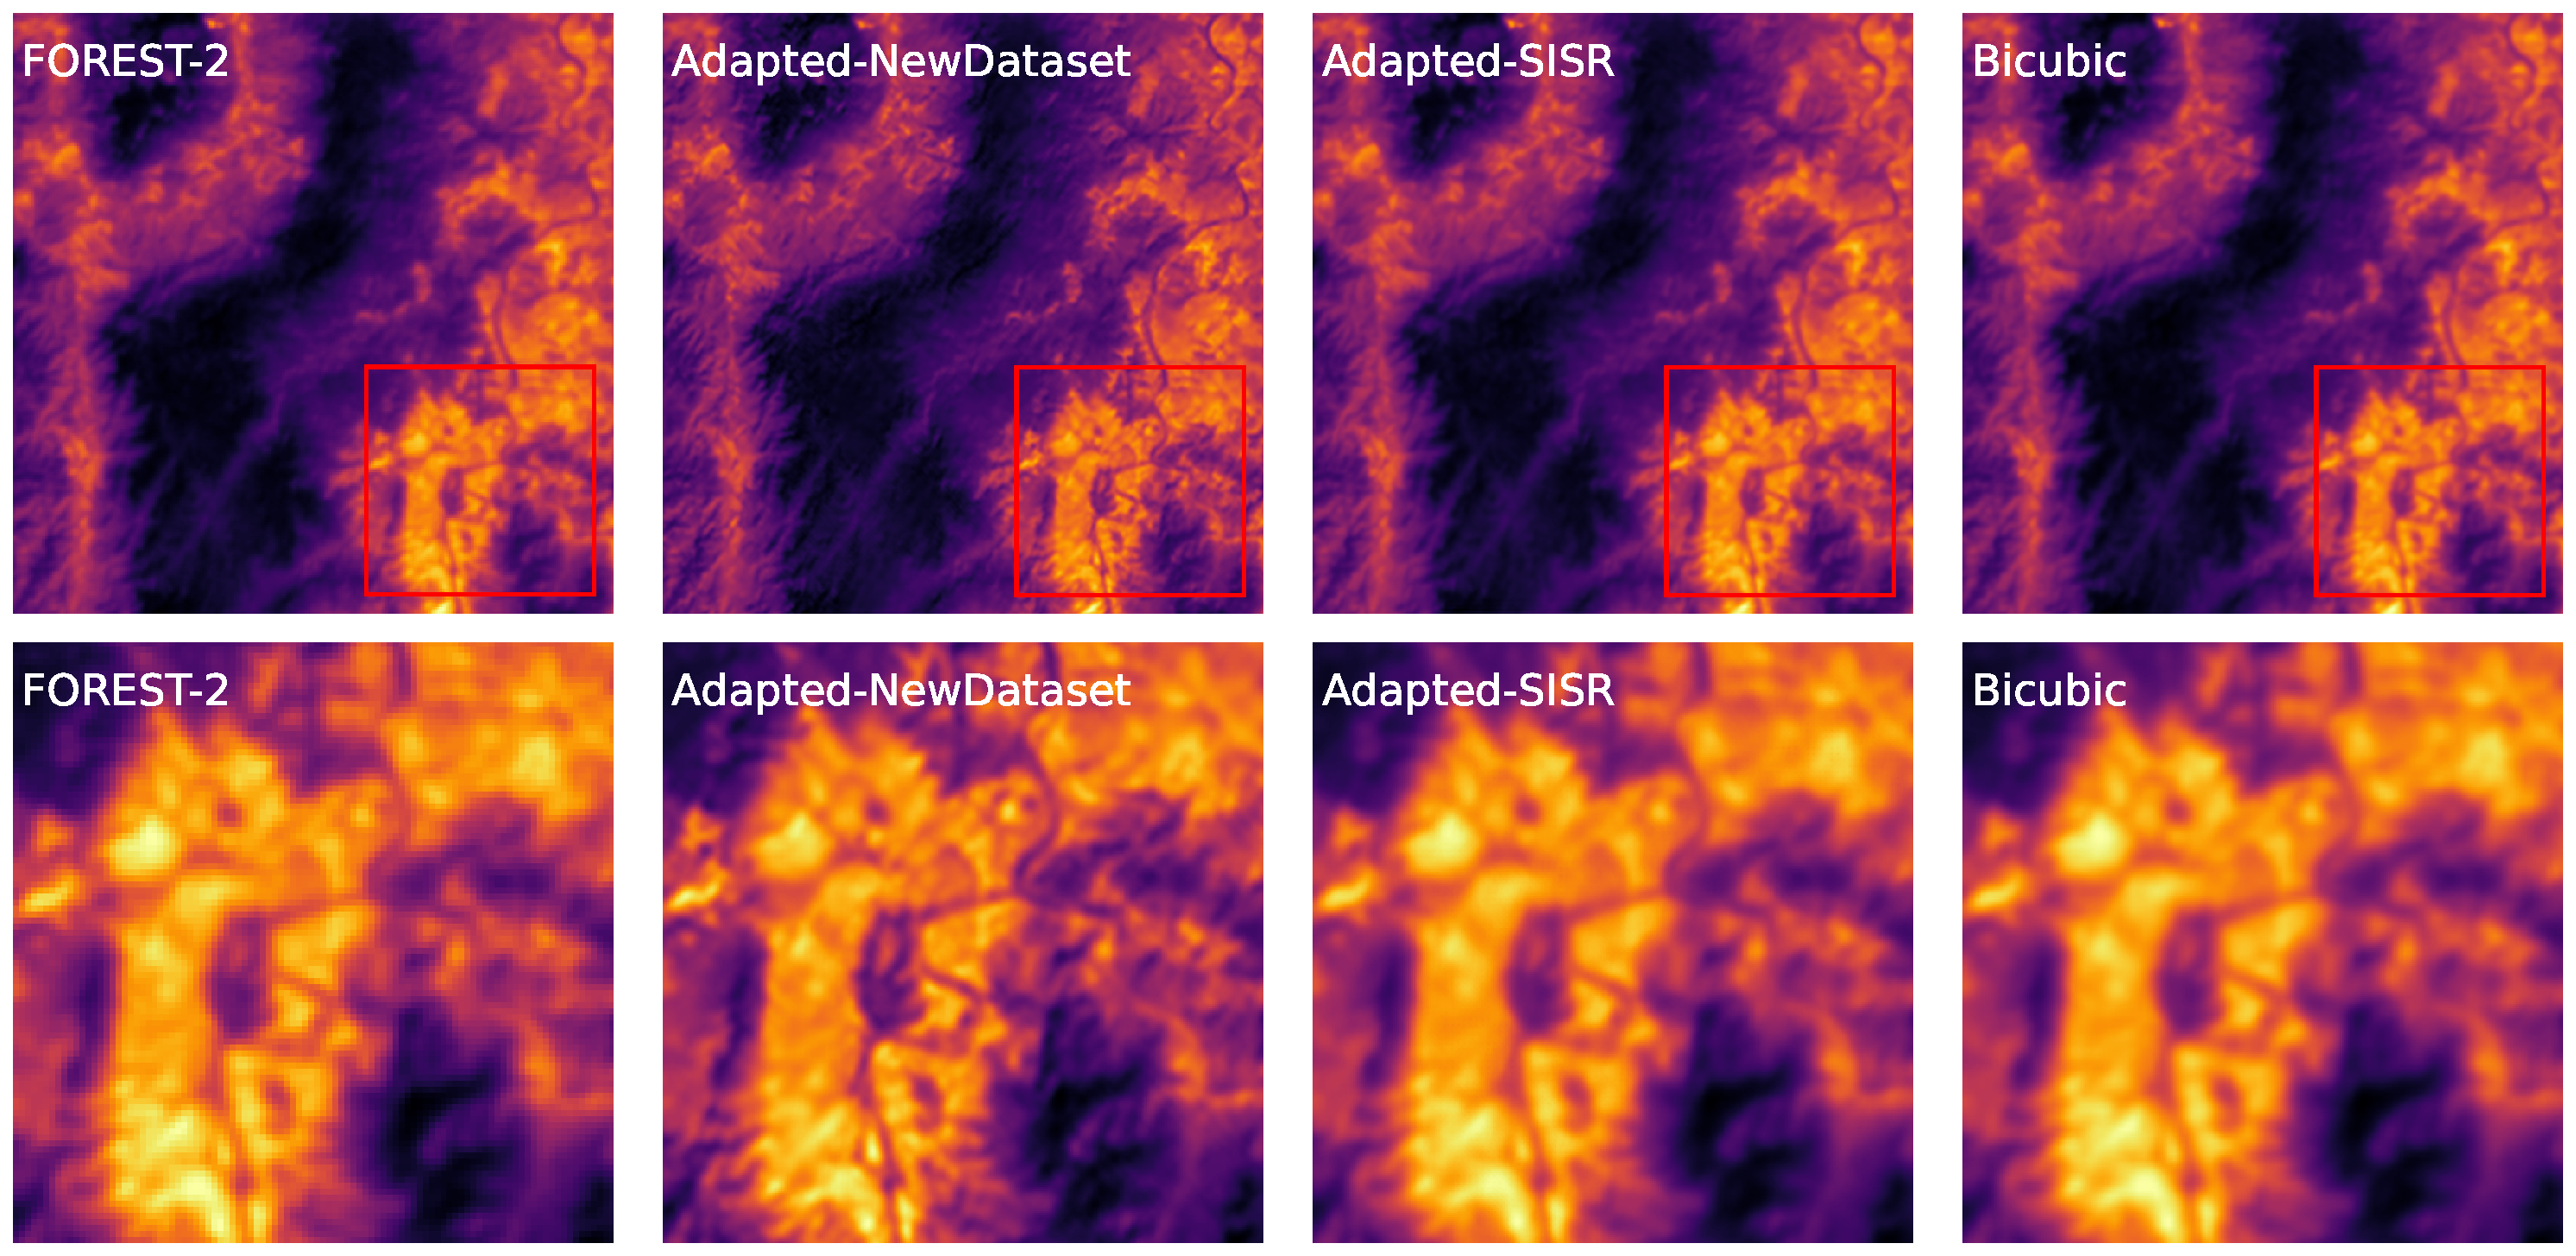
\includegraphics[scale=0.28]{Includes/5-target_prediction_sample.pdf}
            \caption{Super Resolved Forest-2 Scene using different SR models.
                     The image is displayed on the upper row. A detailed zoom is shown below. The original image is displayed on the left, while the super resolved images are displayed on the right.
                    }
            \label{fig:5-target_prediction_sample}
        \end{figure}

        Fig. \ref{fig:5-target-amplification-statistics} shows a more detailed analysis of the frequency domain of the SR images obtained for the whole real FOREST-2 validation dataset.
        In the adapted super resolution, frequency components of interest are amplified in comparison to bicubic upsampling without over-amplifying higher frequencies usually related to noise. Up until 0.3 cycles per pixel, the adapted model has a higher log magnitude than the baseline SR model or bicubic upsampling, also staying slightly higher in high-frequency components.
        As higher frequencies are related to noise and artifacts, this suggests that the adapted model is able to recover more details than the baseline model while minimizing undesired components.
        The amplification plot of the SR models against bicubic upsampling shows the same behavior. 
        The adapted SR amplification increases from the start of the plot and peaks between 0.08 and 0.25 cycles per pixel in a range of between 6 and 8 dB on average. In contrast, the baseline model amplification lies between 0 and 2 dB.
        Such amplification, at a pixel size of 70m, corresponds to cycle frequencies between  300 $\frac{1}{m}$ and 875 $\frac{1}{m}$, which are consistent with the lost frequency components observed in Fig. \ref{fig:5-lr-images-fft-comparison}.
        
        While the amplification is very similar in frequencies related to noise, the adapted model seems to stay higher compared to the baseline.  
        This suggests that the adapted model is able to amplify frequencies of interest at the cost of a slight increase in the overall noise of the image.

        \begin{figure}[H]
            \centering
            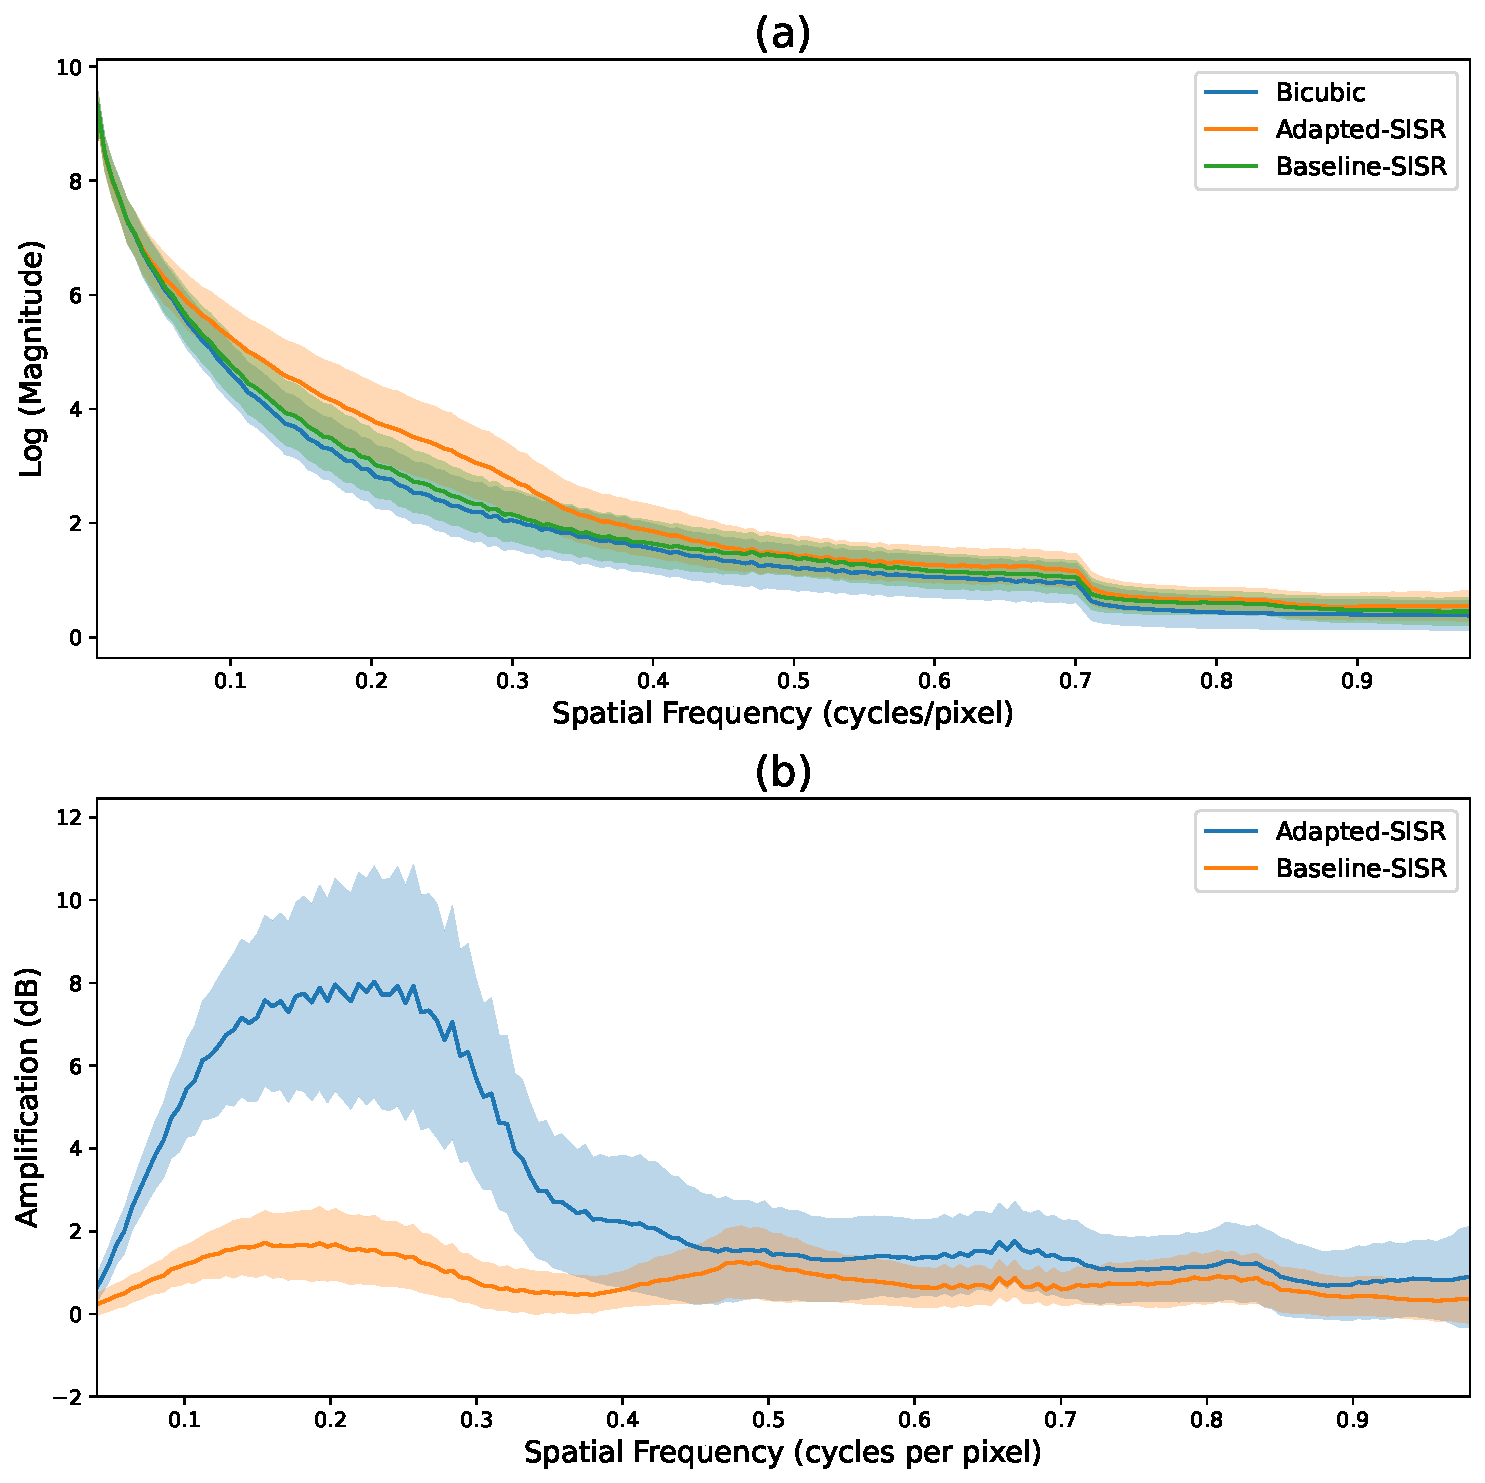
\includegraphics[scale=0.5]{Includes/5-target-amplification-statistics.pdf}
            \caption{Frequency domain analysis of the SR images obtained by applying different SR models to the real FOREST-2 validation dataset.
            In (a), the log of the magnitude of the FFT for the SR images is shown,
            while in (b), the amplification with respect to bicubic upsampling is displayed.}
            \label{fig:5-target-amplification-statistics}
        \end{figure}


        In Fig. \ref{fig:6-target-gradient-analysis-image}, an example of the gradient analysis of the SR images is shown. 
        Compared to the baseline, the adapted SR model shows higher gradient magnitudes. However, in the darker sections of the gradient magnitude, some slight background noise can be observed, consistent with a slightly increased amplification in the higher components of the frequency domain analysis from Fig. \ref{fig:5-target-amplification-statistics}.

        \begin{figure}[H]
            \centering
            \includegraphics[scale=0.28]{Includes/6-target-gradient-analysis-image.pdf}
            \caption{Gradient analysis of the super-resolved images using different SR models for scenes coming from the real FOREST-2 validation dataset.
                     The image is displayed in the upper row. The gradients in the x and y directions ($G_x$ and $G_y$ respectively) are displayed below.
                     the gradient magnitude $|G|$ is displayed in the bottom row.}
            \label{fig:6-target-gradient-analysis-image}
        \end{figure}

        Fig \ref{fig:5-gradient-histogram-validation-dataset} shows the estimated distribution function of the log gradient magnitudes of the whole validation dataset.
        Both the adapted and the baseline models show a decrease in the number of pixels with low gradient magnitudes compared to bicubic upsampling, suggesting that both models are able to recover more details. 
        However, the adapted SR tends to have higher gradient magnitude pixels, implying that the adapted model is able to produce sharper edges than the baseline model.
        This is consistent with the observed results and the frequency domain analysis.
        
        \begin{figure}[H]
            \centering
            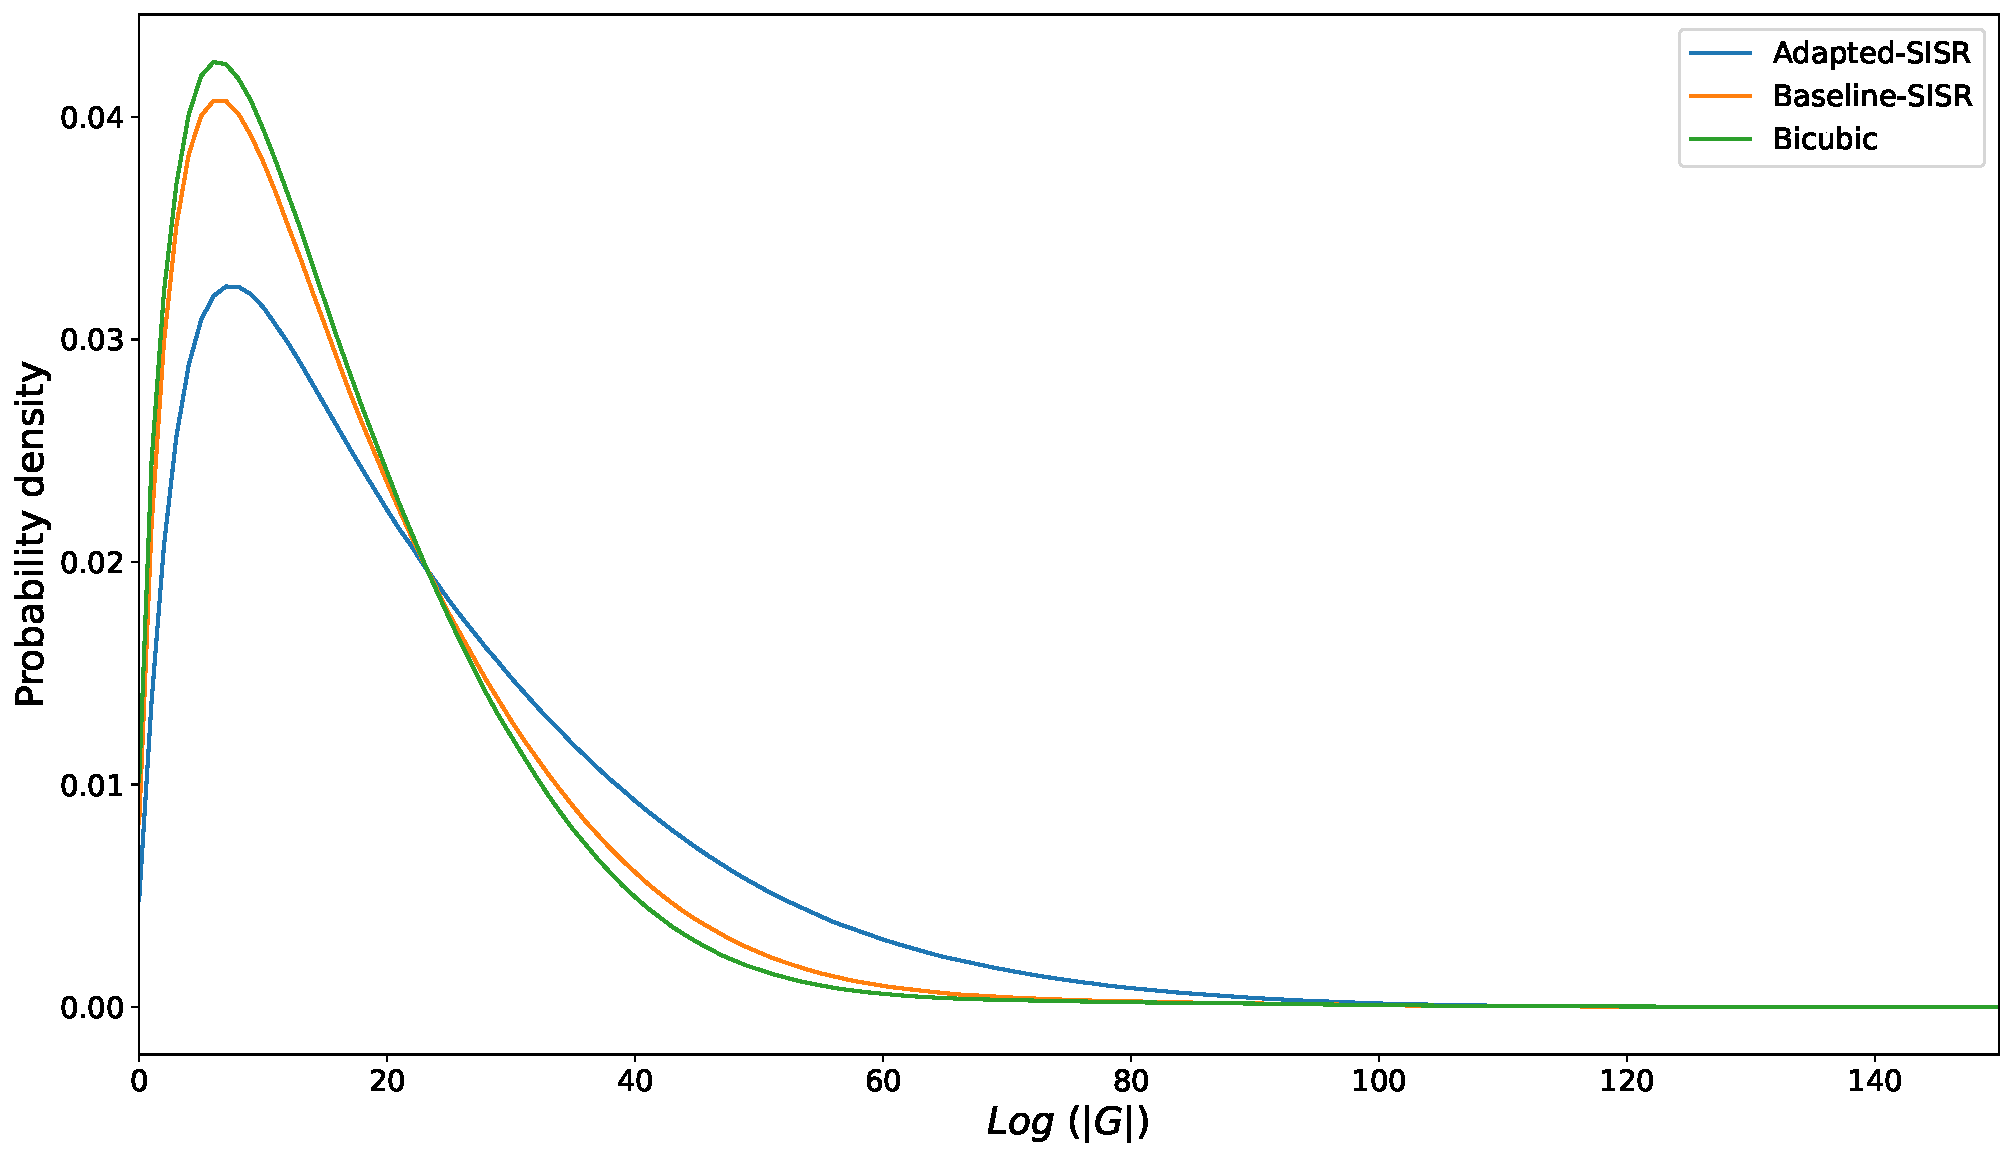
\includegraphics[scale=0.4]{Includes/5-gradient-histogram-validation-dataset.pdf}
            \caption{Density estimation of the gradient magnitude $|G|$ for the super-resolved real FOREST-2 images from the validation dataset. The magnitudes of the Synthetic HR FOREST-2 images are also computed for comparison.}
            \label{fig:5-gradient-histogram-validation-dataset}
        \end{figure}

        In Fig. \ref{fig:5-correlation-histogram-validation-dataset}, the estimated density of the correlation coefficient between the pixels of an image and their neighbors is displayed for the whole validation dataset. 
        As expected for an image, the correlation is extremely high, and the density is highly concentrated. The baseline and bicubic upsampling models have a very similar distribution, with the baseline SR being slightly skewed to the left in comparison.
        The adapted model has a broader distribution that is less dense when closer to 1, implying that the pixels tend to be less correlated with their neighborhood. 
        
        \begin{figure}[H]
            \centering
            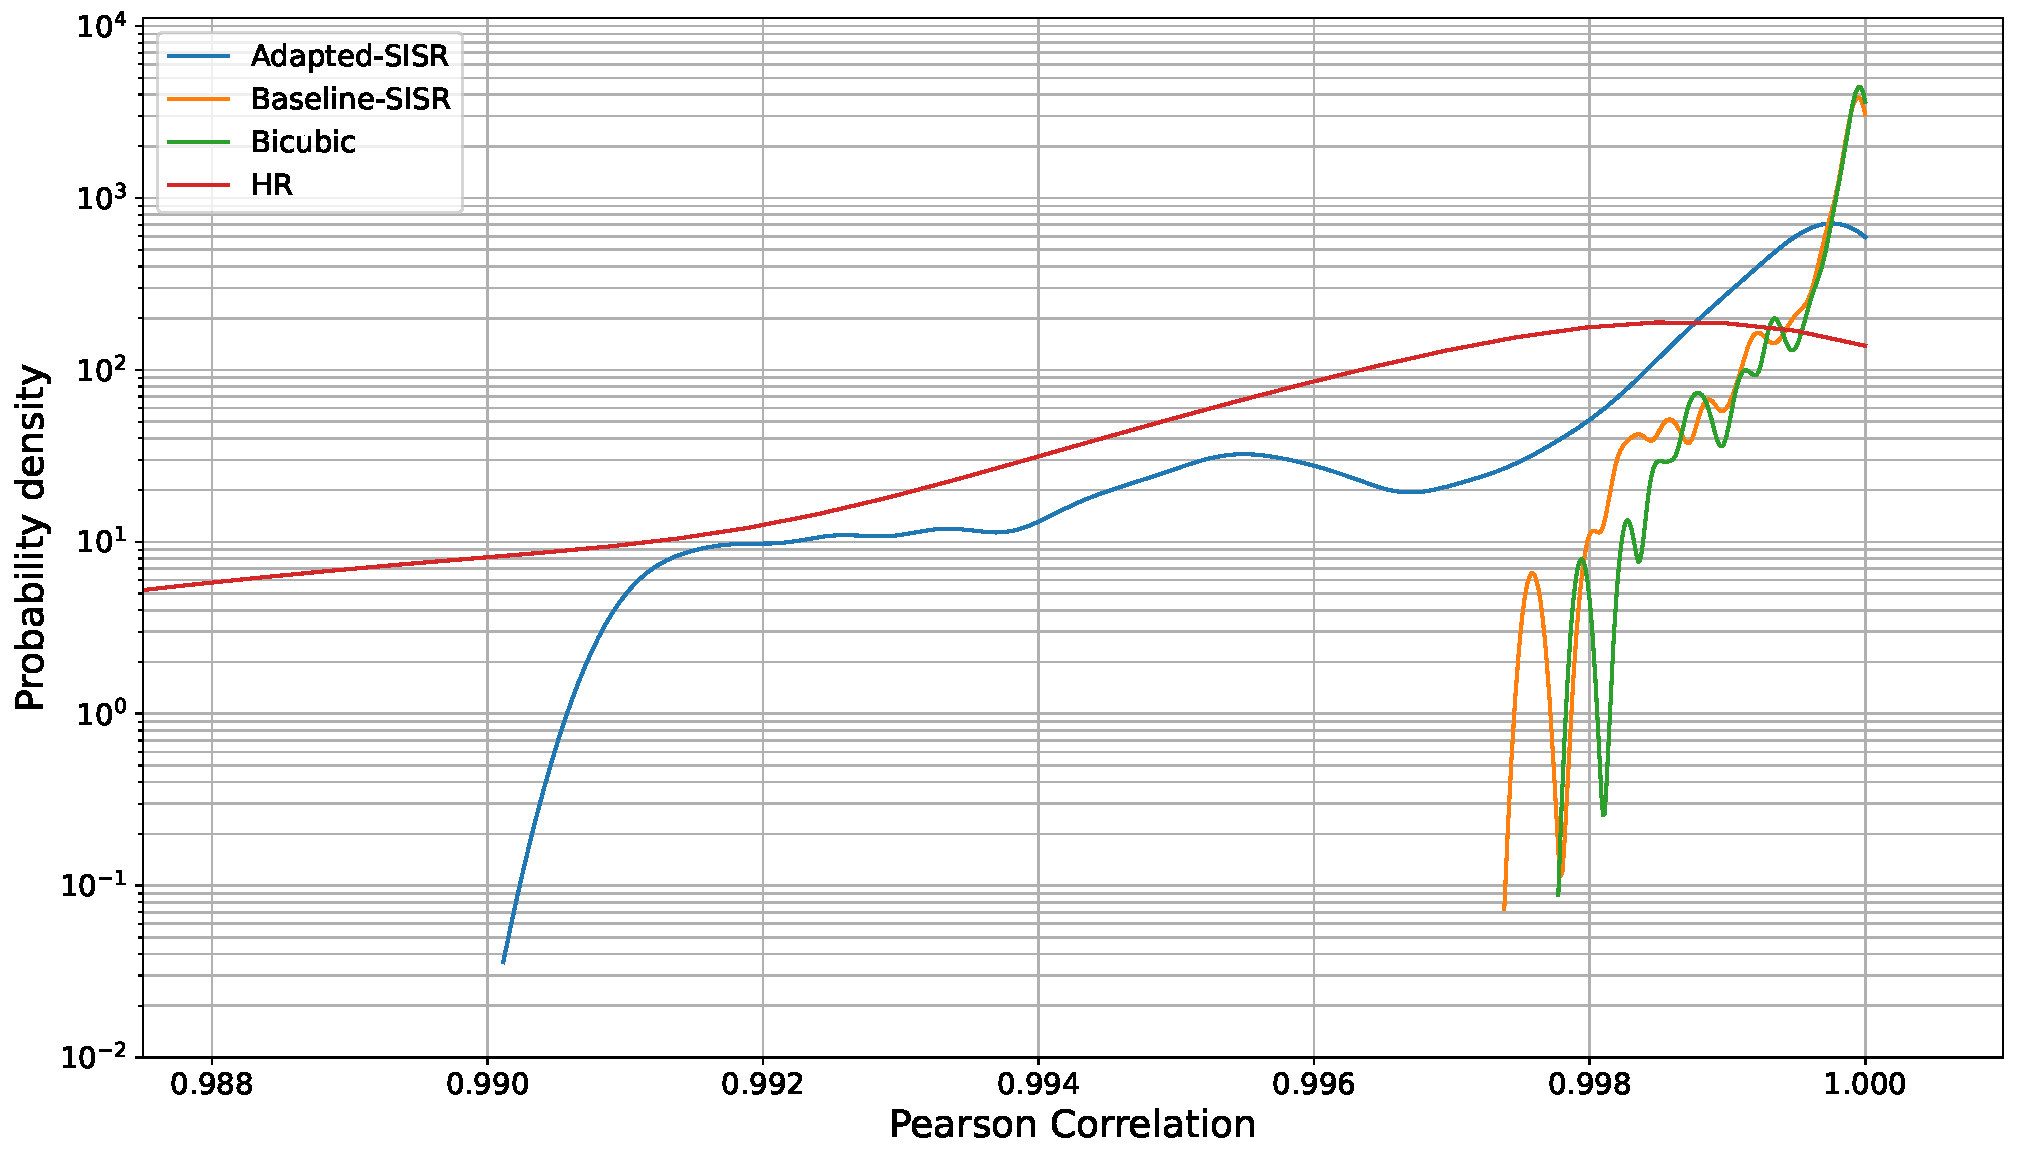
\includegraphics[scale=0.35]{Includes/5-correlation-histogram-validation-dataset.pdf}
            \caption{Density estimation of the correlation coefficient between the pixels and their neighborhoods for the super-resolved real FOREST-2 images from the validation dataset. The coefficients of the synthetic HR FOREST-2 images are also computed for comparison.}
            \label{fig:5-correlation-histogram-validation-dataset}
        \end{figure}

    \subsection{Sensibility to domain shifts}
    
        The combination of the probabilistic degradation model and the SR model was proven helpful to bridge the domain gap and improve the resolution of real FOREST-2 images.
        However, it is important to understand what happens when an arbitrary LR input is not aligned with the target domain seen initially during training.
        While the typical scenario is that the real degradation model is more complex than the one assumed in the dataset generation, the opposite can also occur.
        As seen in \ref{subsec:results-lr-comparison}, assuming a more complex degradation model in the dataset could lead to LR inputs with more attenuation in critical frequency components, resulting in an SR model that over-amplifies to generate an HR output, leading to noisy images with undesired artifacts.
        
        In this particular experiment, HR-LR pairs generated using the baseline degradation model exemplify an overly optimistic degradation scenario and will be used on the SR models of each pipeline.
        As in this experiment, the ground truth is known, the performance of the SR model can be evaluated using metrics like PSNR and SSIM. Additionally, a frequency domain analysis can be performed with respect to the ground truth.
        
        The results are shown in Figs. \ref{fig:5-target-prediction-with-domain-gap} and \ref{fig:5-target-prediction-with-domain-gap-fft}.
        The performance of the adapted model on LR images coming from the baseline degradation model is considerably lower, producing several artifacts and yielding a PSNR difference of approximately 10 dB.

        \begin{figure}[H]
            \centering
            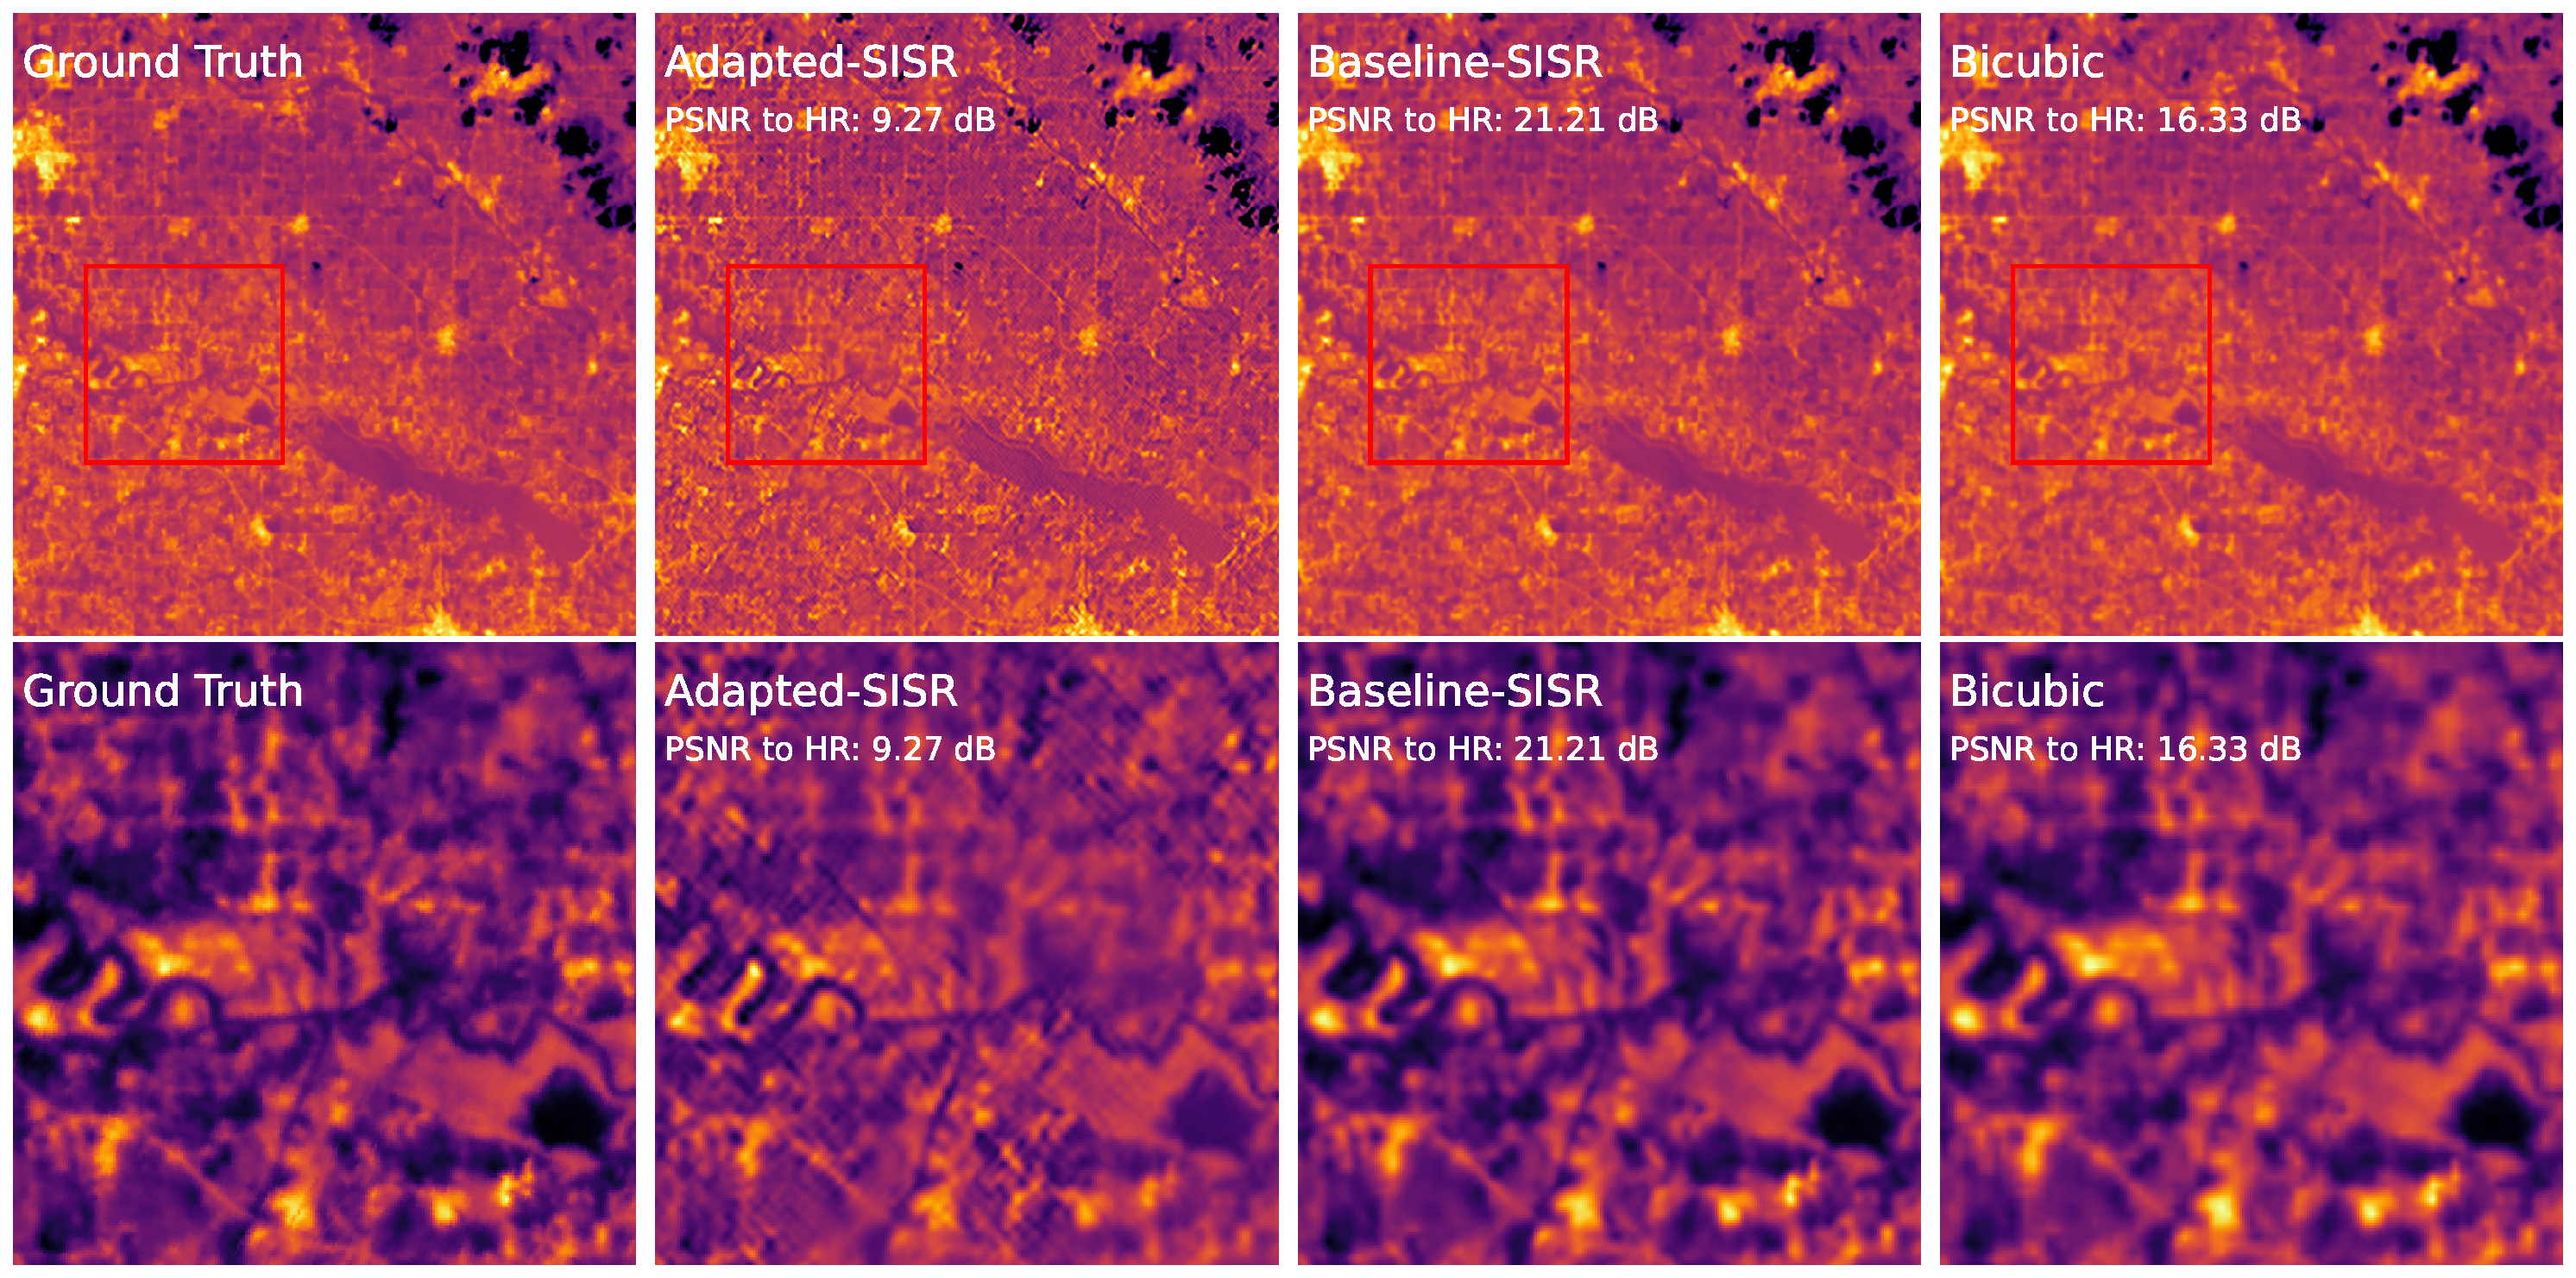
\includegraphics[scale=0.28]{Includes/5-target_prediction_sample-with-domain-gap.pdf}
            \caption{Effects of using a model trained on a different domain than at inference time. 
                     When using an HR image degraded with the baseline degradation model as an input, the model trained using real FOREST-2 data as the target domain generates several artifacts and underperforms severely in terms of PSNR. }
            \label{fig:5-target-prediction-with-domain-gap}
        \end{figure}

        The frequency domain analysis of the ground truth and the super-resolved images are shown in Fig. \ref{fig:5-target-prediction-with-domain-gap-fft}.  
        The adapted model amplifies frequencies with respect to the ground truth, something that should not happen in any SR task. 
        This suggests that while the adapted model may highlight edges and details, it also severely amplifies the noise and artifacts, resulting in a worse performance in terms of PSNR.
        

        \begin{figure}[H]
            \centering
            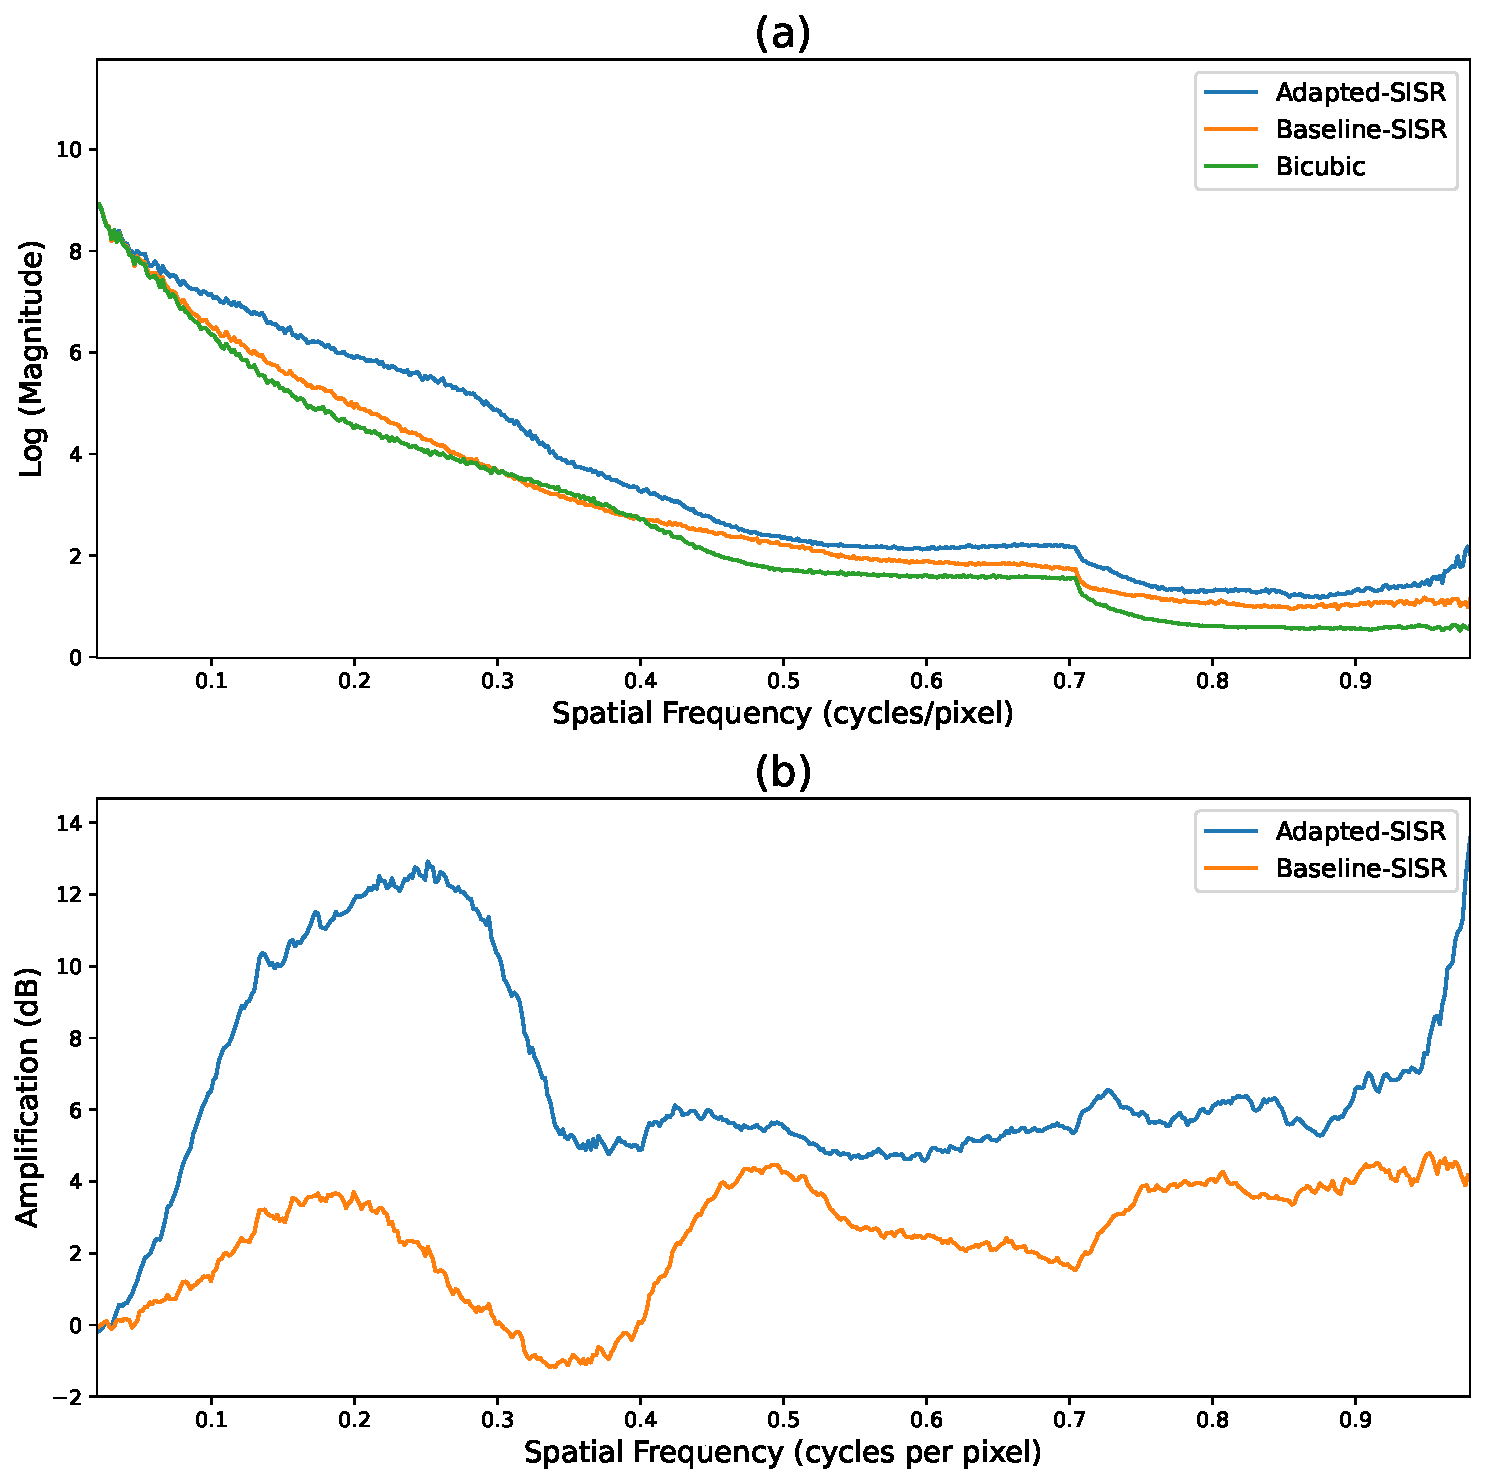
\includegraphics[scale=0.4]{Includes/5-target-prediction-with-domain-gap-fft.pdf}
            \caption{Effects of using a model trained with on different domain than at inference time. (a) shows the log magnitude of the radial average of the FFT for the SR images using different algorithms. (b) shows the amplification with respect to the ground truth.}
            \label{fig:5-target-prediction-with-domain-gap-fft}
        \end{figure}

        Fig \ref{fig:5-target-amplification-statistics-with-domain-gap} shows the results of the frequency domain analysis for the whole validation dataset. The results seem to be consistent with the range observed in Fig. \ref{fig:5-target-prediction-with-domain-gap-fft}. Having frequency amplification with respect to the ground truth is a display of the inability of the adapted SR model to reconstruct the ground truth image properly.
        
        The adapted model was trained on generated LR images that try to mimic the real FOREST-2 images, which have a more complex degradation model. This results in an SR model that attempts to reconstruct the ground truth from a worse starting point. The SR model then learns to amplify some frequencies more than needed when the LR images come from the baseline degradation model.


        \begin{figure}[H]
            \centering
            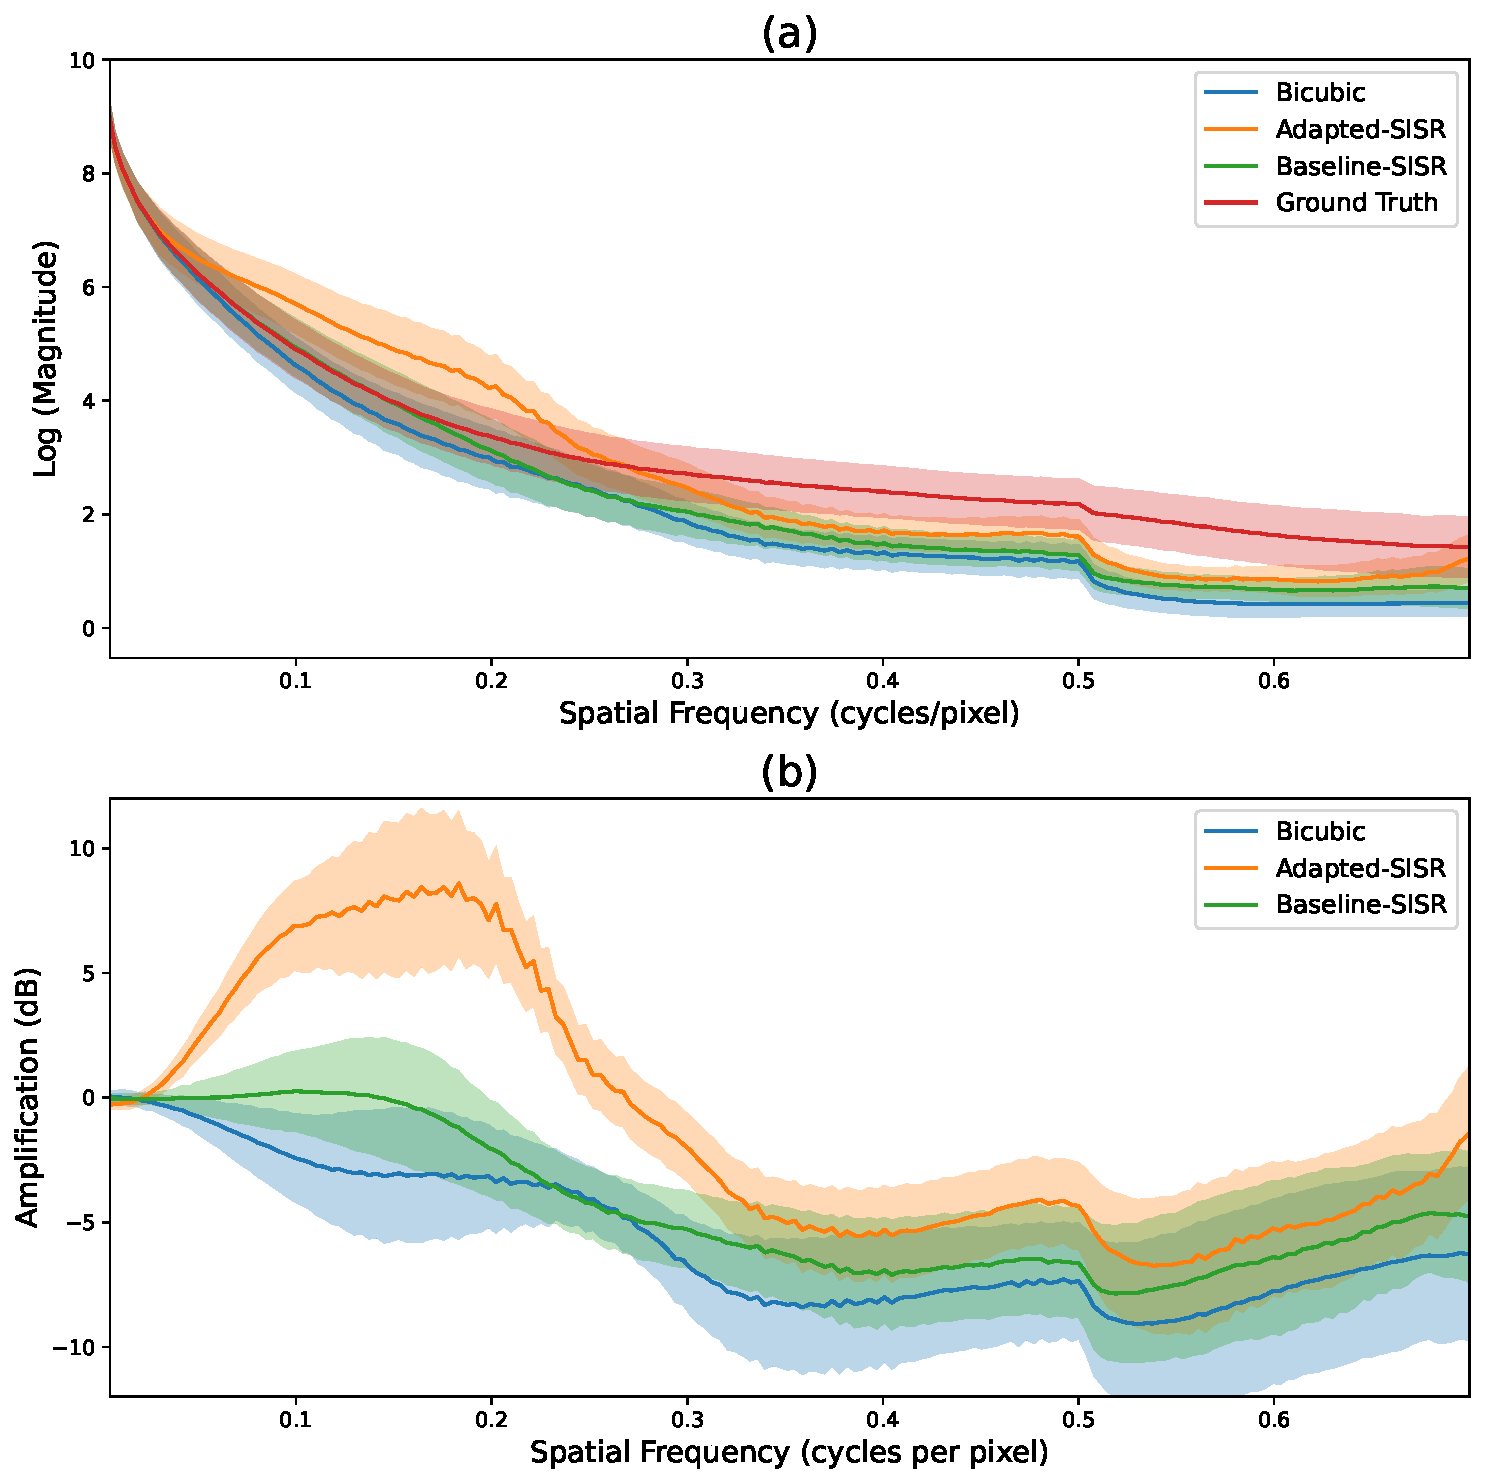
\includegraphics[scale=0.4]{Includes/5-target-amplification-statistics-with-domain-gap.pdf}
            \caption{Effects of using a model trained on a different domain than at inference time, statistics over the whole validation dataset. 
                     (a) shows the log magnitude of the radial average of the FFT for the SR images using different algorithms.
                     (b) shows the amplification with respect to the ground truth.
                     Painted areas represent ±1 standard deviations.
                     }
            \label{fig:5-target-amplification-statistics-with-domain-gap}
        \end{figure}

        The performance results in terms of different metrics are shown in Fig. \ref{fig:5-target-prediction-with-domain-gap-dataset}. 
        In the conditions described above, the adapted super resolution model underperforms severely in every considered metric.


        \begin{figure}[H]
            \centering
            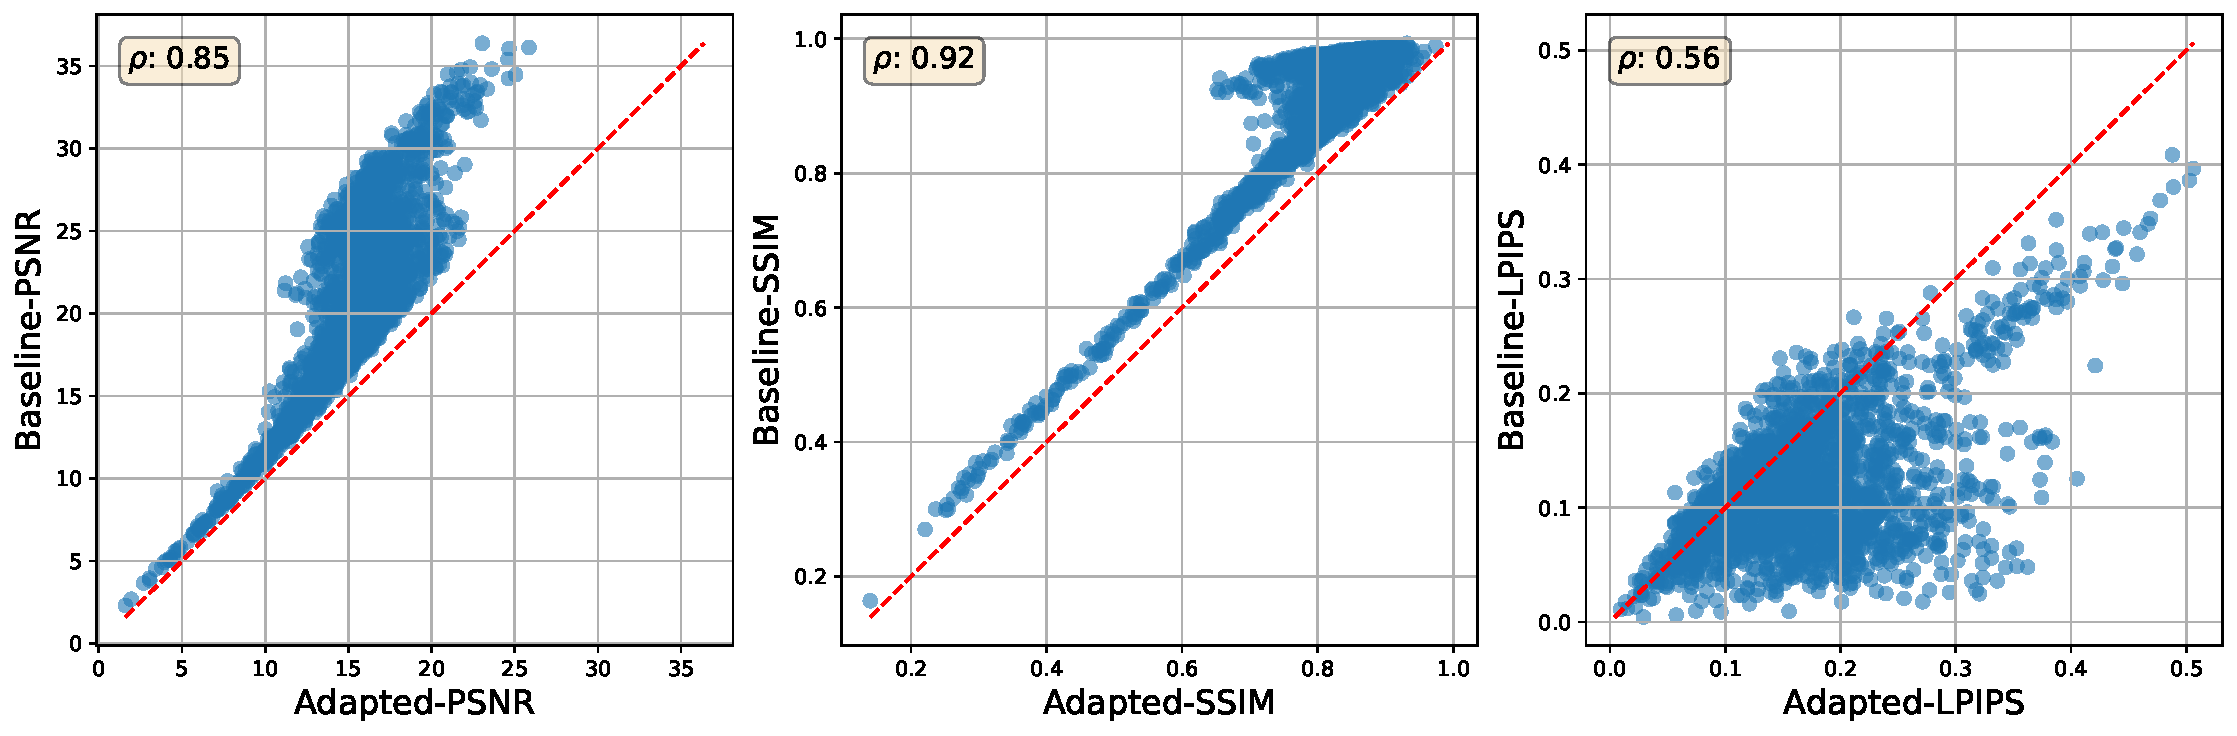
\includegraphics[scale=0.38]{Includes/5-target-prediction-with-domain-gap-dataset.pdf}
            \caption{Performance obtained by super resolving the degraded synthetic FOREST images using different super resolution models. The Pearson correlation coefficient is represented by $\rho$.}
            \label{fig:5-target-prediction-with-domain-gap-dataset}
        \end{figure}


    Another example of a domain shift happens when a faulty scene is taken from FOREST-2. The response of the SR models can be seen in Fig. \ref{fig:target-prediction-with-domain-gap-from-forest-.pdf}. The stripe noise present in the LR input is exacerbated, and the image has a grainy texture, clearly performing worse with respect to the baseline. This is confirmed with the log magnitude and amplification plots from Fig. \ref{fig:5-target-prediction-with-domain-gap-from-forest-fft.pdf}, where the adapted SISR continues to amplify between 4dB and 6dB for frequencies above 0.25 cycles per pixel, introducing a lot of noise.


     \begin{figure}[H]
        \centering
        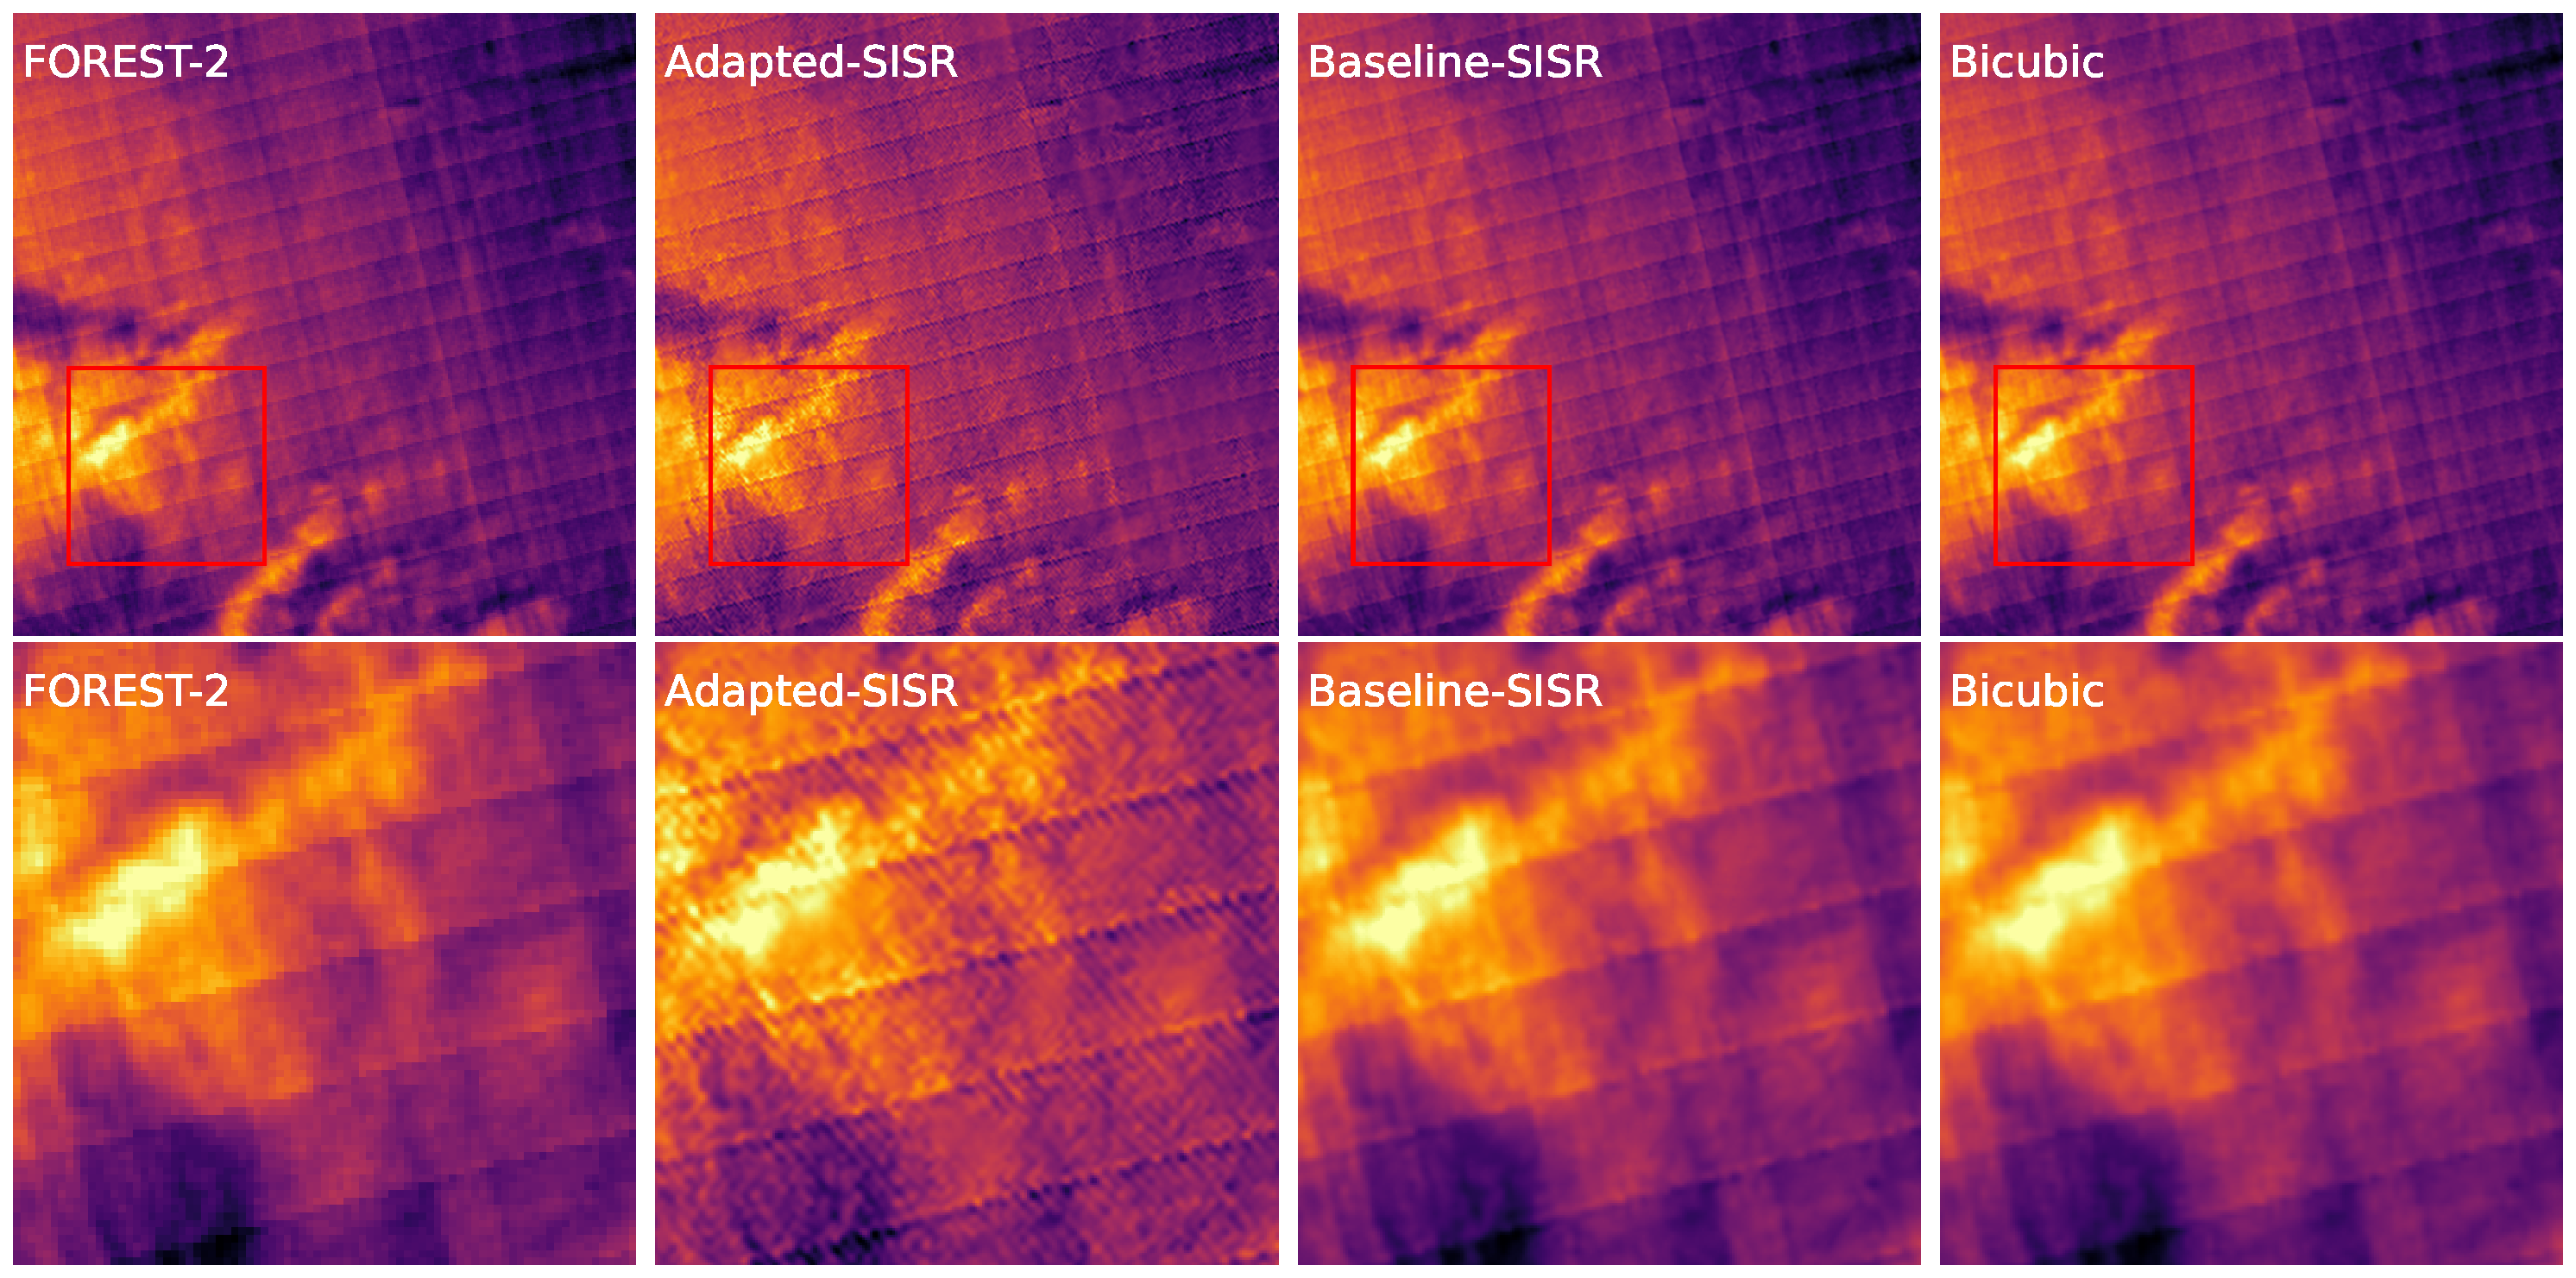
\includegraphics[width=\textwidth]{Includes/5-target-prediction-with-domain-gap-from-forest-.pdf}
        \caption{\small{ Effects of using a faulty FOREST-2 image on the SR models. The adapted model introduces noise and increases the stripe noise present in the image.}}
        \label{fig:target-prediction-with-domain-gap-from-forest-.pdf}
    \end{figure}

 \begin{figure}[H]
        \centering
        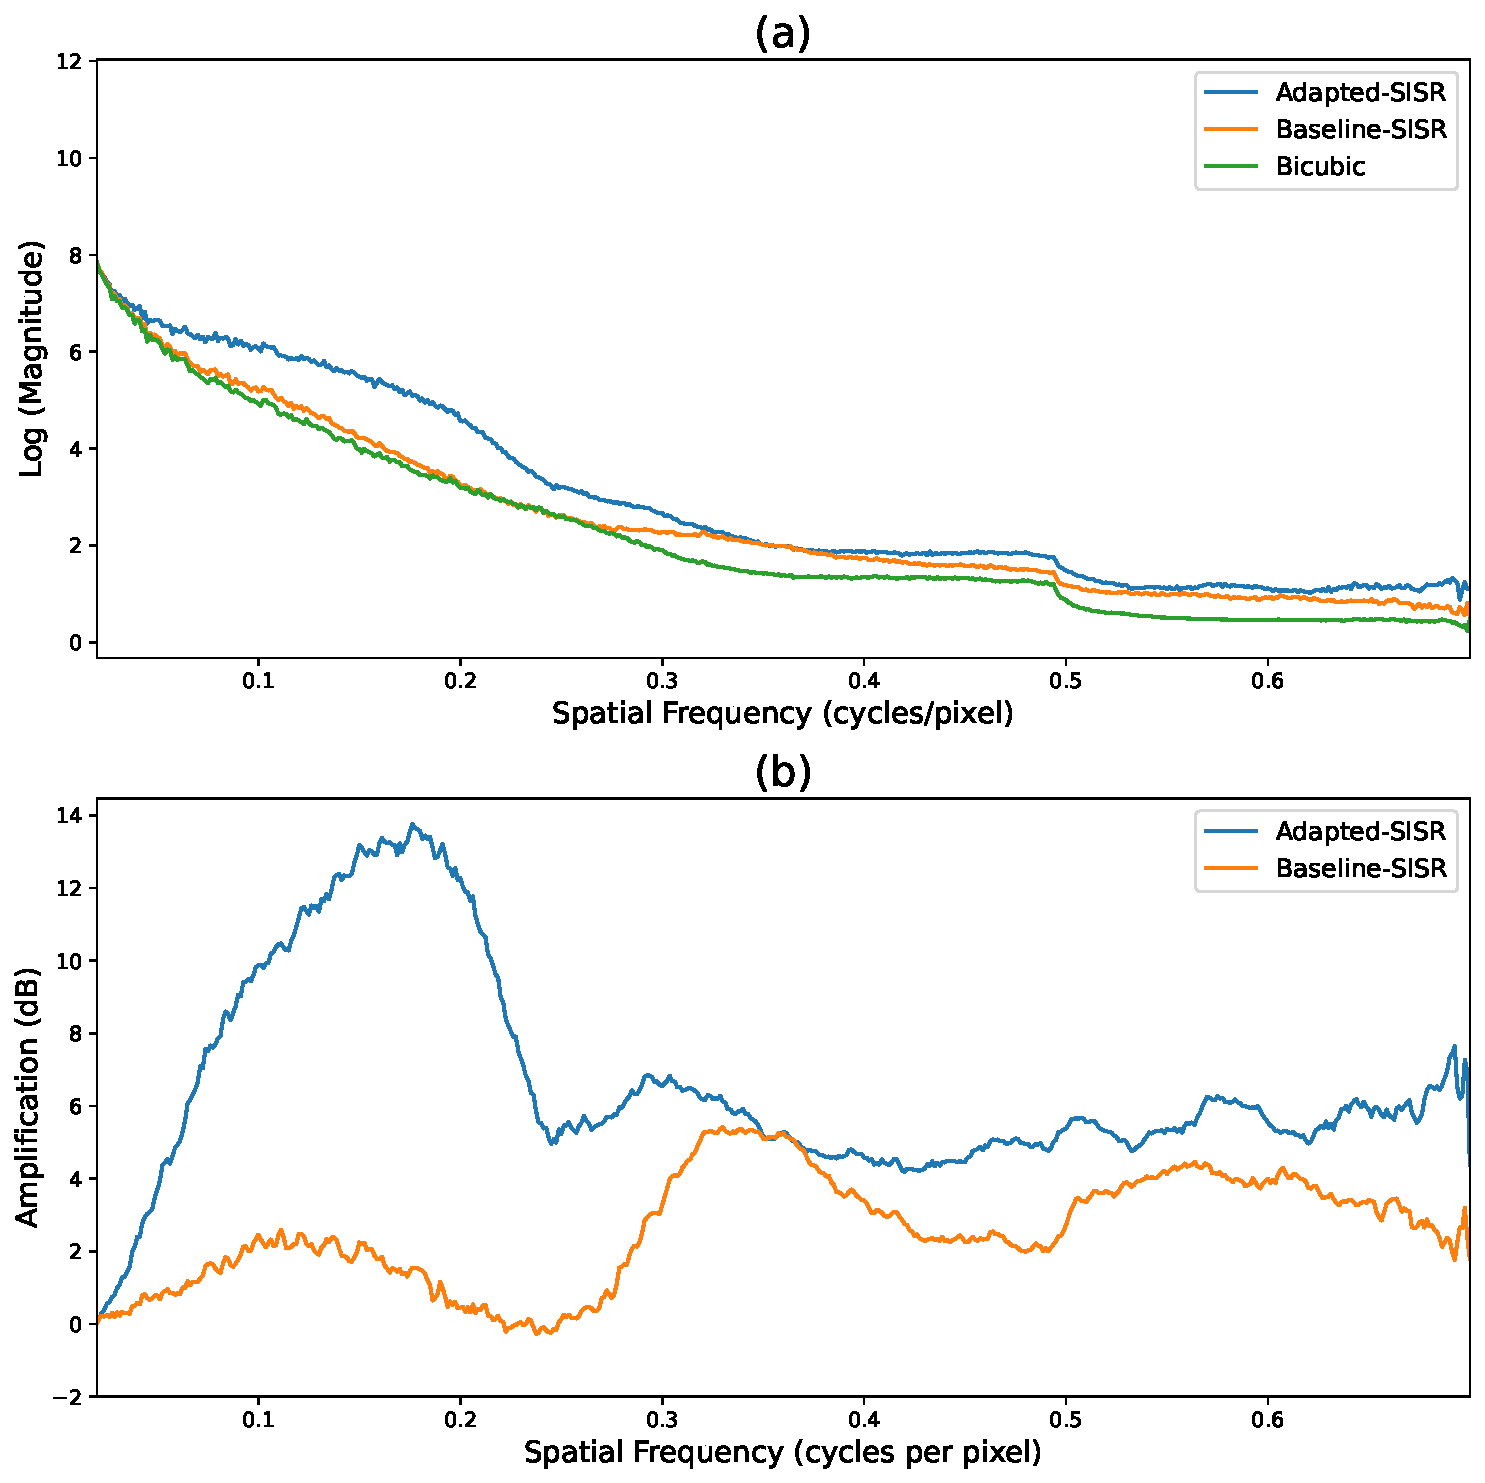
\includegraphics[scale= 0.38]{Includes/5-target-prediction-with-domain-gap-from-forest-fft.pdf}
        \caption{\small{Effects of using a faulty FOREST-2 image on the SR models, analyzed in the frequency domain. (a) shows the log amplitude of the super resolution outputs. (b) shows the amplification with respect to bicubic interpolation.}}
        \label{fig:5-target-prediction-with-domain-gap-from-forest-fft.pdf}
    \end{figure}
    
    Both examples demonstrate that while this approach is very good for bridging the domain gap, it is not robust at all to domain shifts. The model will not perform well if the input comes from a different degradation model or even if the input FOREST-2 data is not of a similar quality as the ones seen in training. Pre-processing methods that detect faulty images are vital to determine if performing super resolution is advisable. 
    The observed limitation is in sync with what was found in the literature seen in \ref{subsubsec:implicit-modelling}. Implicit modeling for blind super resolution using GANs is not able to generalize to arbitrary images not seen during training.

    \subsubsection{Assessment using non-referenced image quality metrics}
    
    NRIQA metrics can help to understand the relative performance of the SR models when arbitrary LR images are used as input. The analysis was performed by taking the adapted and baseline SR models and using them to super resolve LR images coming from the baseline degradation and real LR forest-2 images.
    Then, the NIQE and BRISQUE scores were calculated.
    
    The results are shown in Fig. \ref{fig:5-target-iqa-results}.
    For both metrics, a significant gap is observed between the adapted model and the rest when the input is real FOREST-2 data.
    This behavior is not replicated when the input LR images are generated using the baseline degradation. Moreover, for the adapted model, both metrics tend to get worse when the input images are not real FOREST-2 images. The contrary happens for the rest of the models.

    \begin{figure}[H]
        \centering
        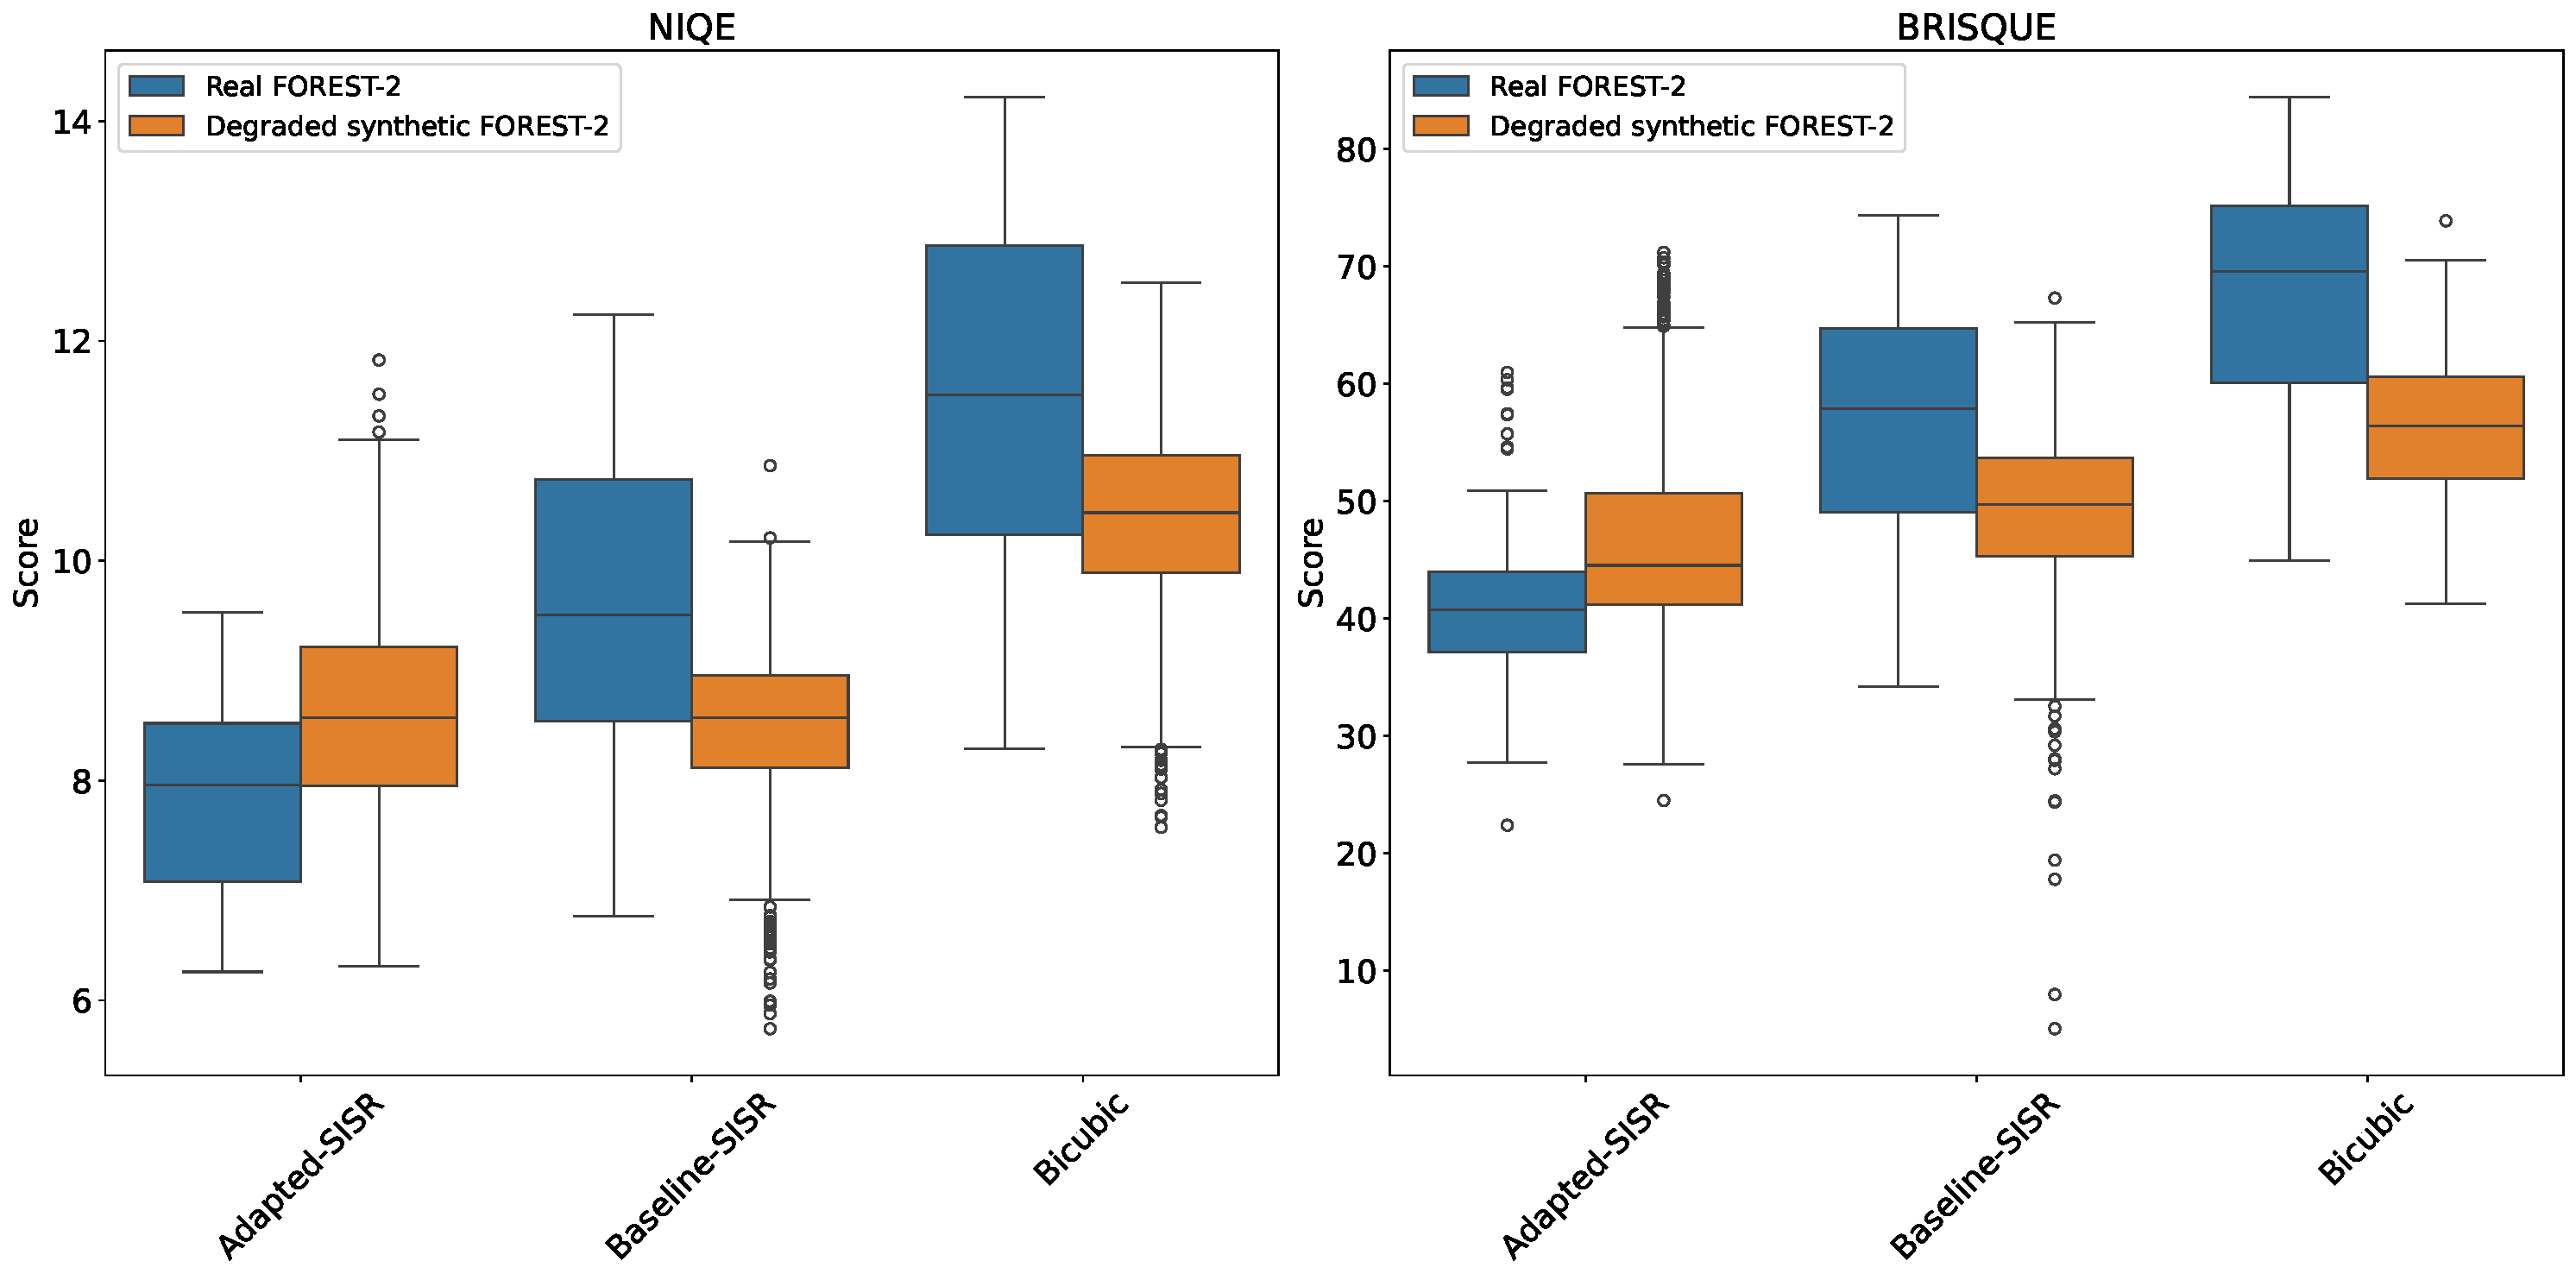
\includegraphics[scale=0.25]{Includes/5-target-iqa-results.pdf}
        \caption{Image quality assessment metrics for the different SR models using different datasets as input. }
        \label{fig:5-target-iqa-results}
    \end{figure}

    
    This suggests that the SR model is able to produce more natural images only when the input images come from the same distribution as the target domain used in training. However, it is important to note that: 

    


    \begin{enumerate}
        \item NIQE and BRISQUE are calculated using a pre-trained model. The images used for the pre-training are not remote sensing images, and therefore, the results may not be representative. This could be circumvented by training a NIQE/BRISQUE model with a more adequate dataset for the task.
        \item NIQE and BRISQUE are a measure of image quality and naturalness, not physical consistency or reconstruction fidelity.
    \end{enumerate}

    \subsection{Performance evaluation on paired data}


        In this subsection, the performance of the SR models on the single paired scene described in Sec. \ref{subsec:pairedacquisition} will be evaluated. The scene is located in the South Thompson River, British Columbia, Canada. A depiction of it is shown in Fig. \ref{fig:5-crossover-performance}

        For this single scene, the adapted SR model had better performance compared to the baseline SR and bicubic upsampling. Notably, a distinct dark spot clearly visible in the magnified view is accurately reconstructed in the adapted SR, matching the dimensions from the ground truth. This feature is identified as the Copper Island\footnote{\url{https://maps.app.goo.gl/B7XqaRkHndsDdJebA}}, which spans roughly 600 meters in diameter. While the baseline SR and bicubic upsampling barely reveal the land, the adapted SR succeeds in reconstructing it to its corresponding size.
        
        Although the modified SR model shows improved PSNR values, it is important to note that the ECOSTRESS image is affected by stripe noise, a common issue acknowledged by the mission's team \cite{ecostress2018datafaq}. This noise may compromise the integrity of the PSNR metric. Furthermore, the analysis is based on a single scene, which constrains the scope of any conclusions, emphasizing the need for broader data to validate the findings comprehensively.

    \begin{figure}[H]
        \centering
        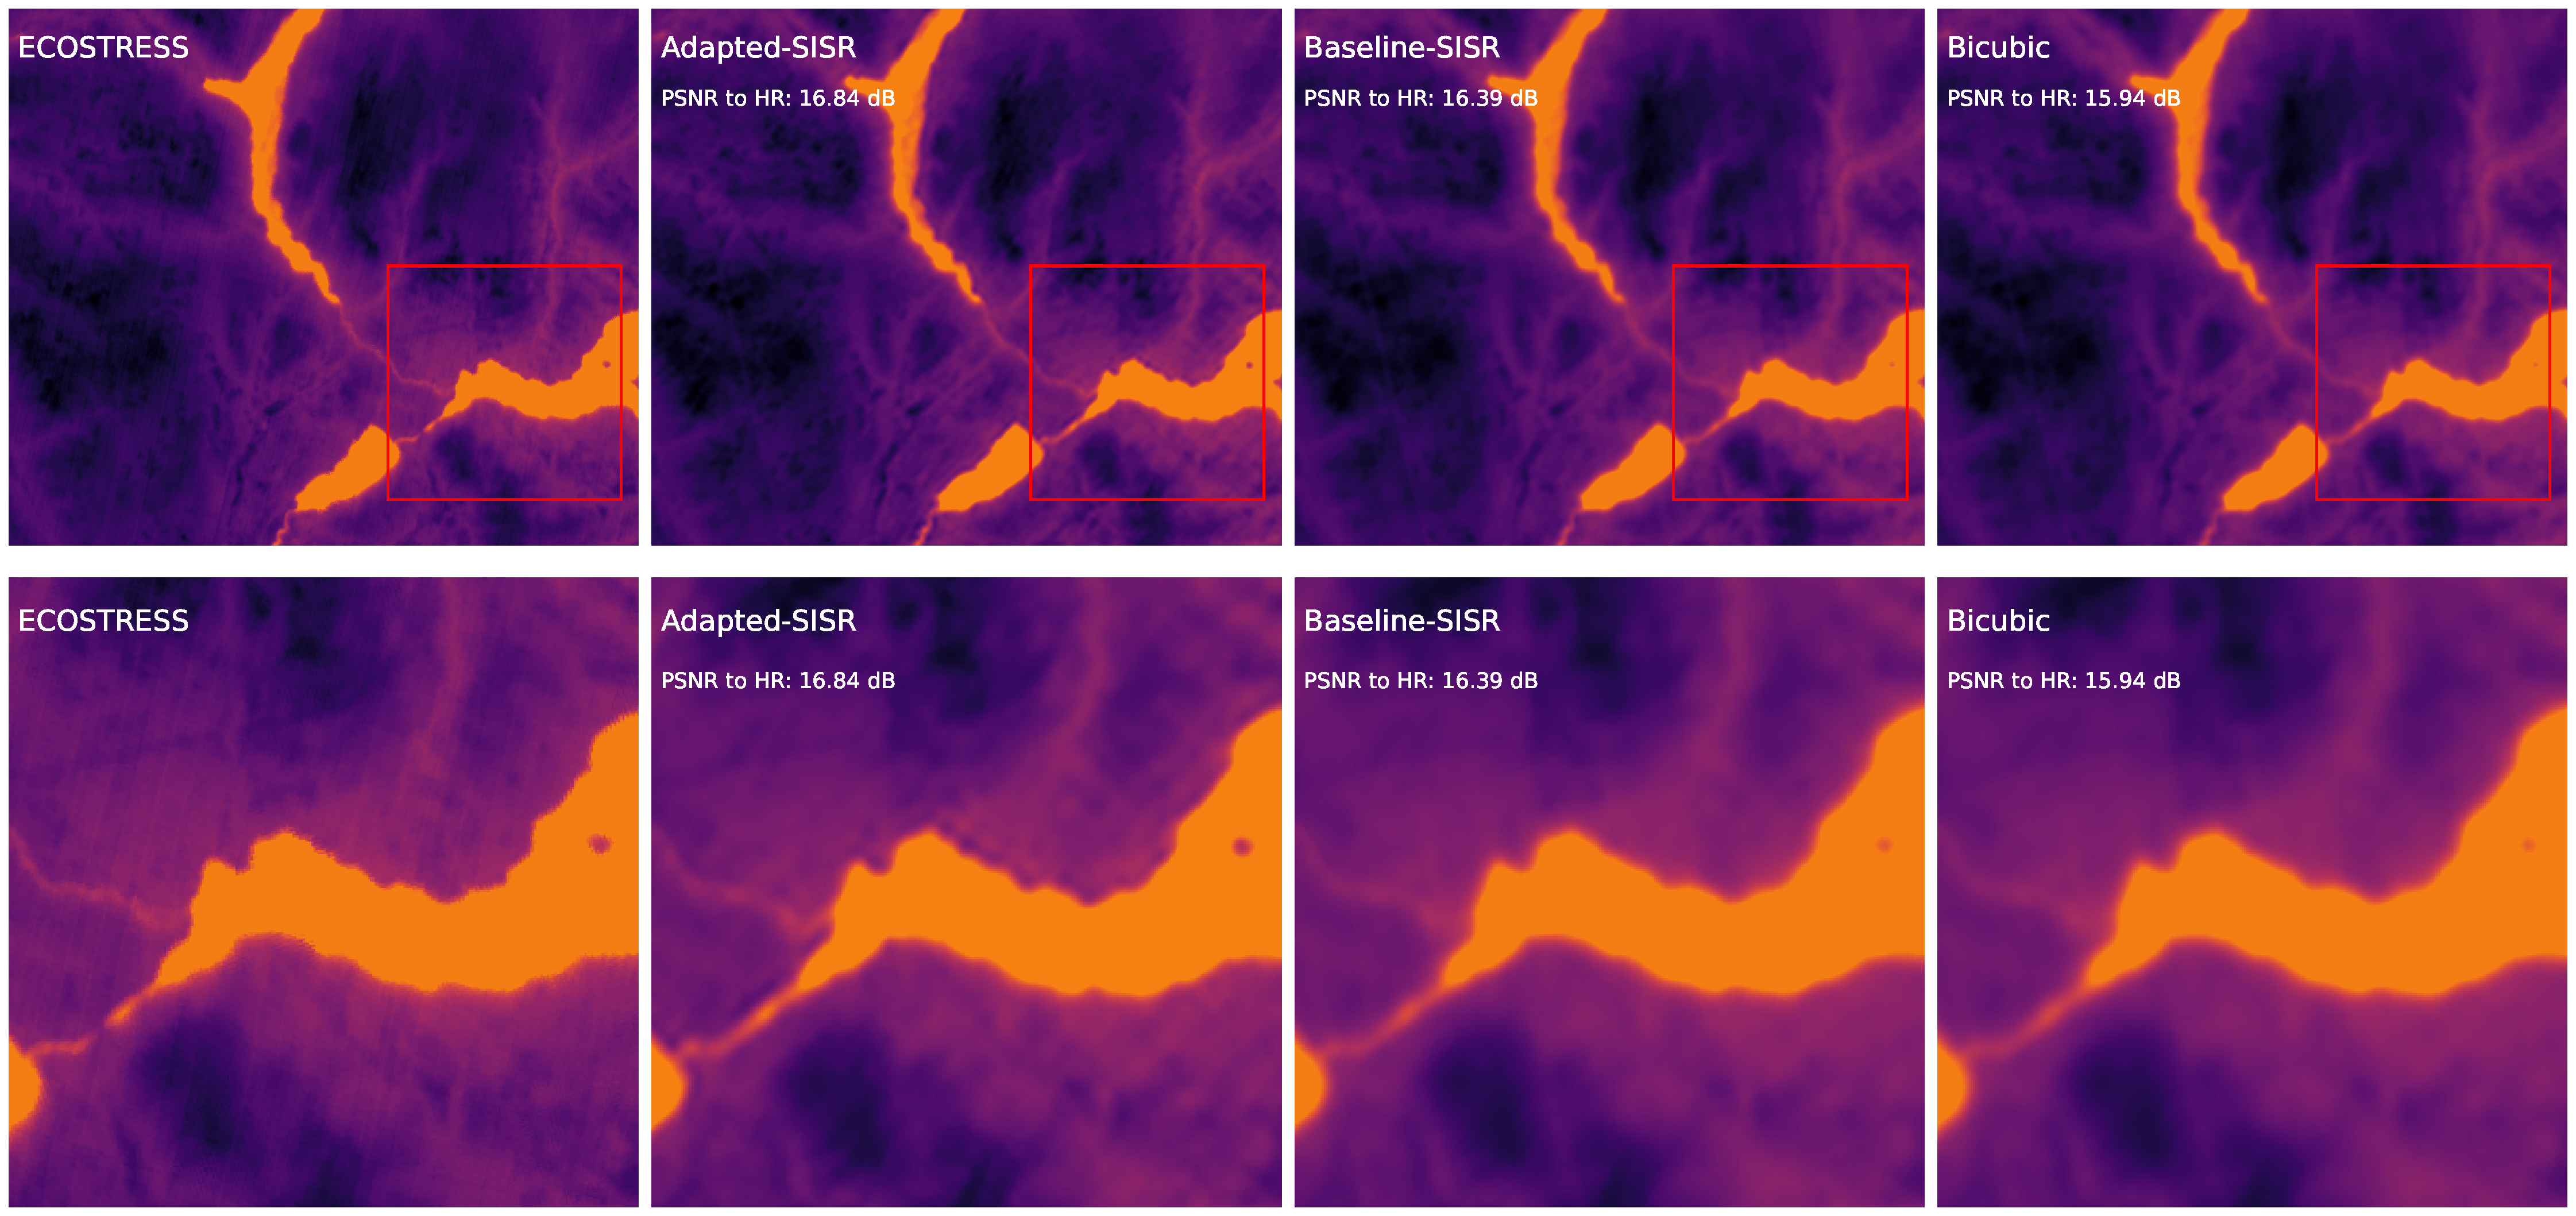
\includegraphics[width=\textwidth]{Includes/5-crossover-performance.pdf}
        \caption{Paired ECOSTRESS and super-resolved FOREST-2 images using different SR models. The scene is displayed in the upper row, and a detailed zoom is shown below. The ECOSTRESS image is shown on the left, while the outputs of each SR method applied on the original FOREST-2 image lie on the right}
        \label{fig:5-crossover-performance}
    \end{figure}


    The FFT analysis of the scene is depicted in Fig. \ref{fig:5-crossover-fft}. Unlike the bicubic and baseline models, the adapted model demonstrates less attenuation, signifying superior retention of image details across various spatial frequencies. This attribute is crucial as it suggests that the adapted model preserves the integrity of the original image more faithfully than its counterparts. Furthermore, an important observation is the absence of amplification in the adapted model's FFT analysis, contrary to what is observed when the input image is not aligned with what was seen in the training data, such as Fig. \ref{fig:5-target-prediction-with-domain-gap-fft}. 

    \begin{figure}[H]
        \centering
        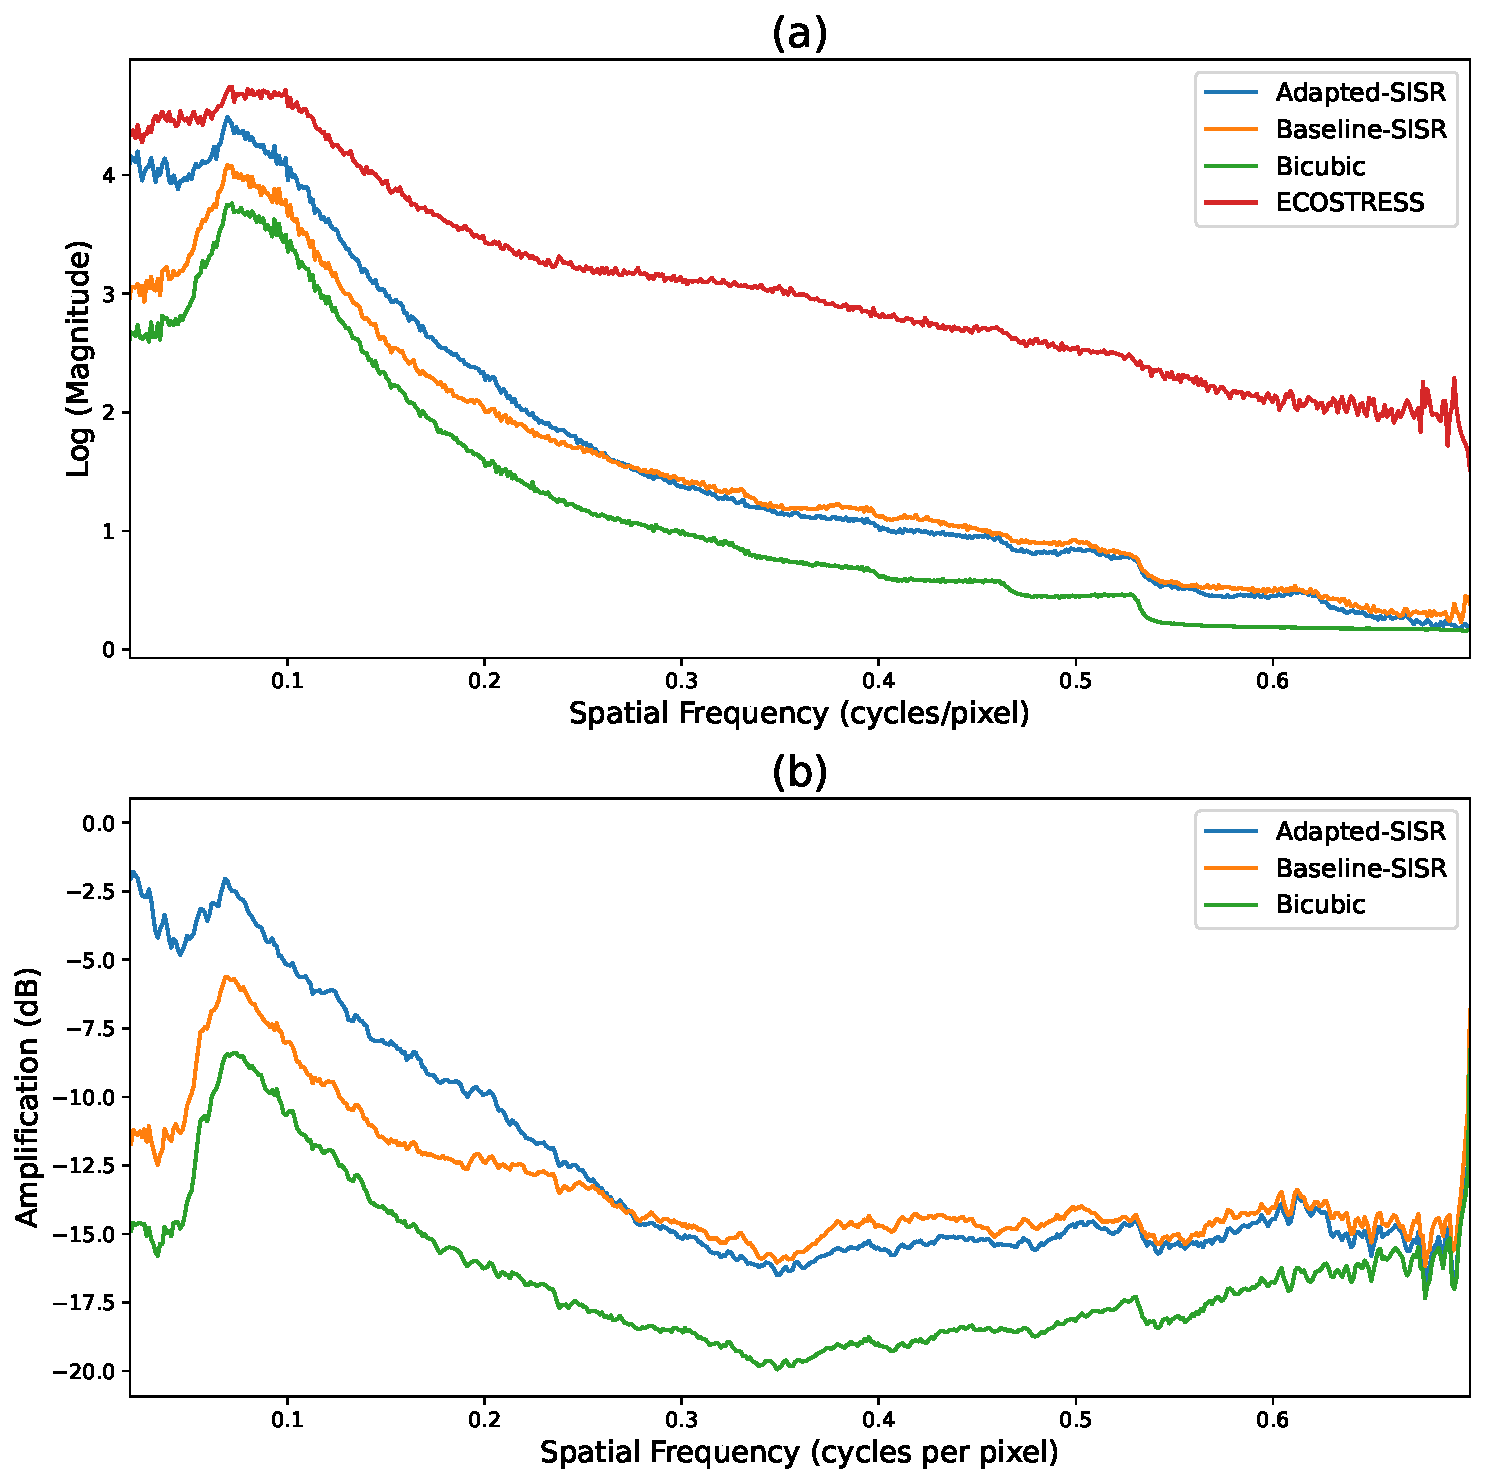
\includegraphics[width=\textwidth]{Includes/5-crossover-performance-fft.pdf}
        \caption{FFT analysis of the scene from Fig. \ref{fig:5-crossover-performance}. (a) shows the log amplitude of the ECOSTRESS and super-resolved outputs. (b) shows the amplification with respect to the ECOSTRESS image.}
        \label{fig:5-crossover-fft}
    \end{figure}

    The gradient analysis and histogram are displayed in Figs. \ref{fig:5-crossover-gradients} and \ref{fig:5-crossover-gradients-histogram}, respectively. The adapted SR model succeeds in generating an image with higher gradient magnitudes, along with a modest reduction in the correlation of each pixel with its neighbors, in comparison to both the baseline SR and bicubic upsampling. This result is consistent with what was observed in the target domain analysis. The comparison with the ground truth shows that there is room for improvement in SR algorithms.

    \begin{figure}[H]
        \centering
        \includegraphics[width=\textwidth]{Includes/5-crossover-gradient.pdf}
        \caption{Gradient magnitudes of the scene from Fig. \ref{fig:5-crossover-performance}. The image is displayed in the upper row. The gradients in the x and y directions ($G_x$ and $G_y$ respectively) are displayed below. the gradient magnitude $|G|$ is displayed in the bottom row.}
        \label{fig:5-crossover-gradients}
    \end{figure}

    \begin{figure}[H]
        \centering
        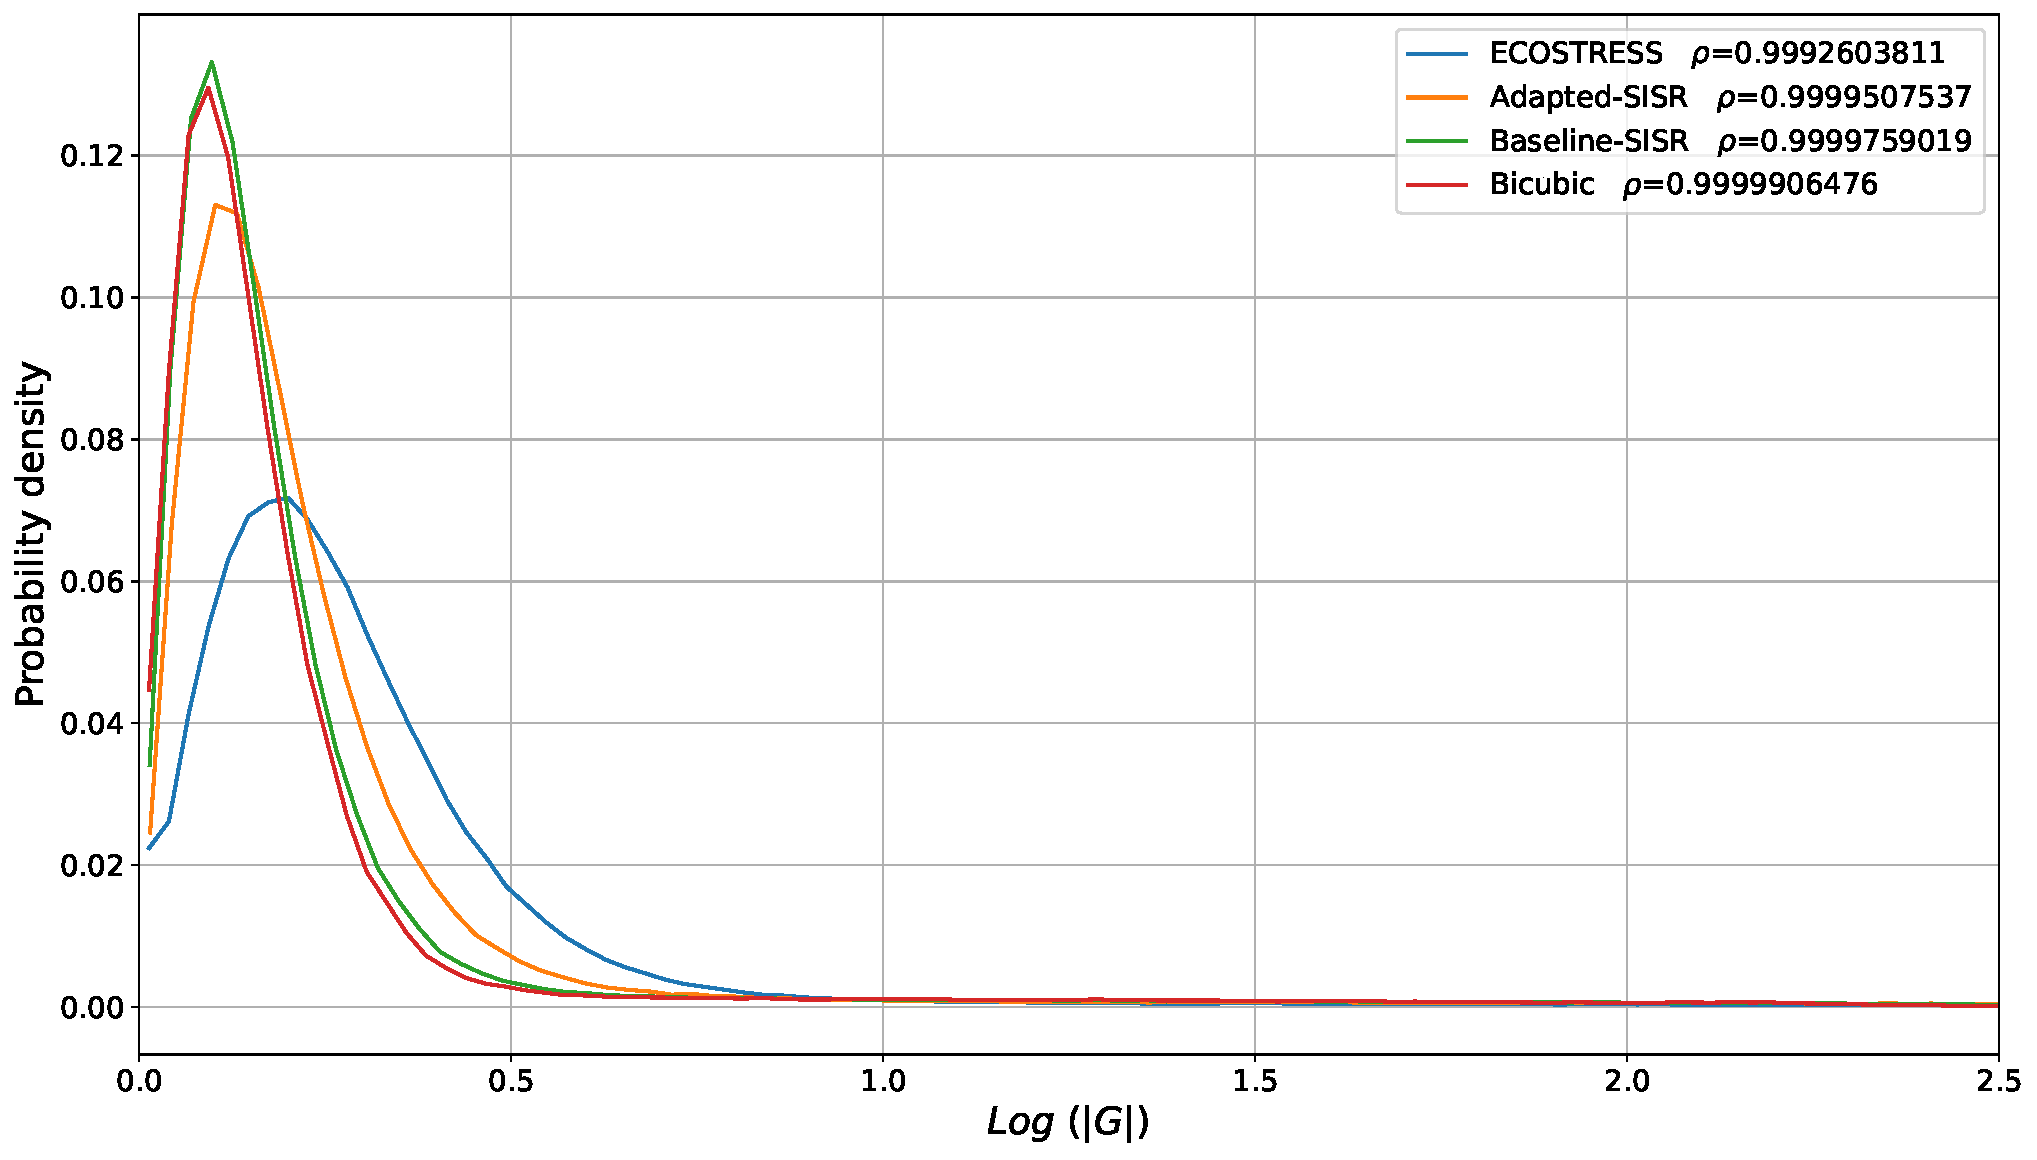
\includegraphics[width=\textwidth]{Includes/5-crossover-gradient-histogram.pdf}
        \caption{Histogram of the gradient magnitudes from Fig. \ref{fig:5-crossover-gradients}. The correlation coefficient between each pixel and its neighbors for each image is computed as $\rho$ in the legend. }
        \label{fig:5-crossover-gradients-histogram}
    \end{figure}
    

    To further understand the model performance, a thousand random crops of 400-pixel size are extracted, and the PSNR of each crop is calculated. The results are displayed in Fig. \ref{fig:5-crossover-fft-scatter}. The adapted SR model showed consistently better performance than the baseline SR and bicubic upsampling methods. However, the margin of improvement is not overwhelmingly large. Moreover, the baseline SR exhibits lower performance than bicubic upsampling,  highlighting the limitations of traditional degradation models in real-world super resolution tasks.


    \begin{figure}[H]
        \centering
        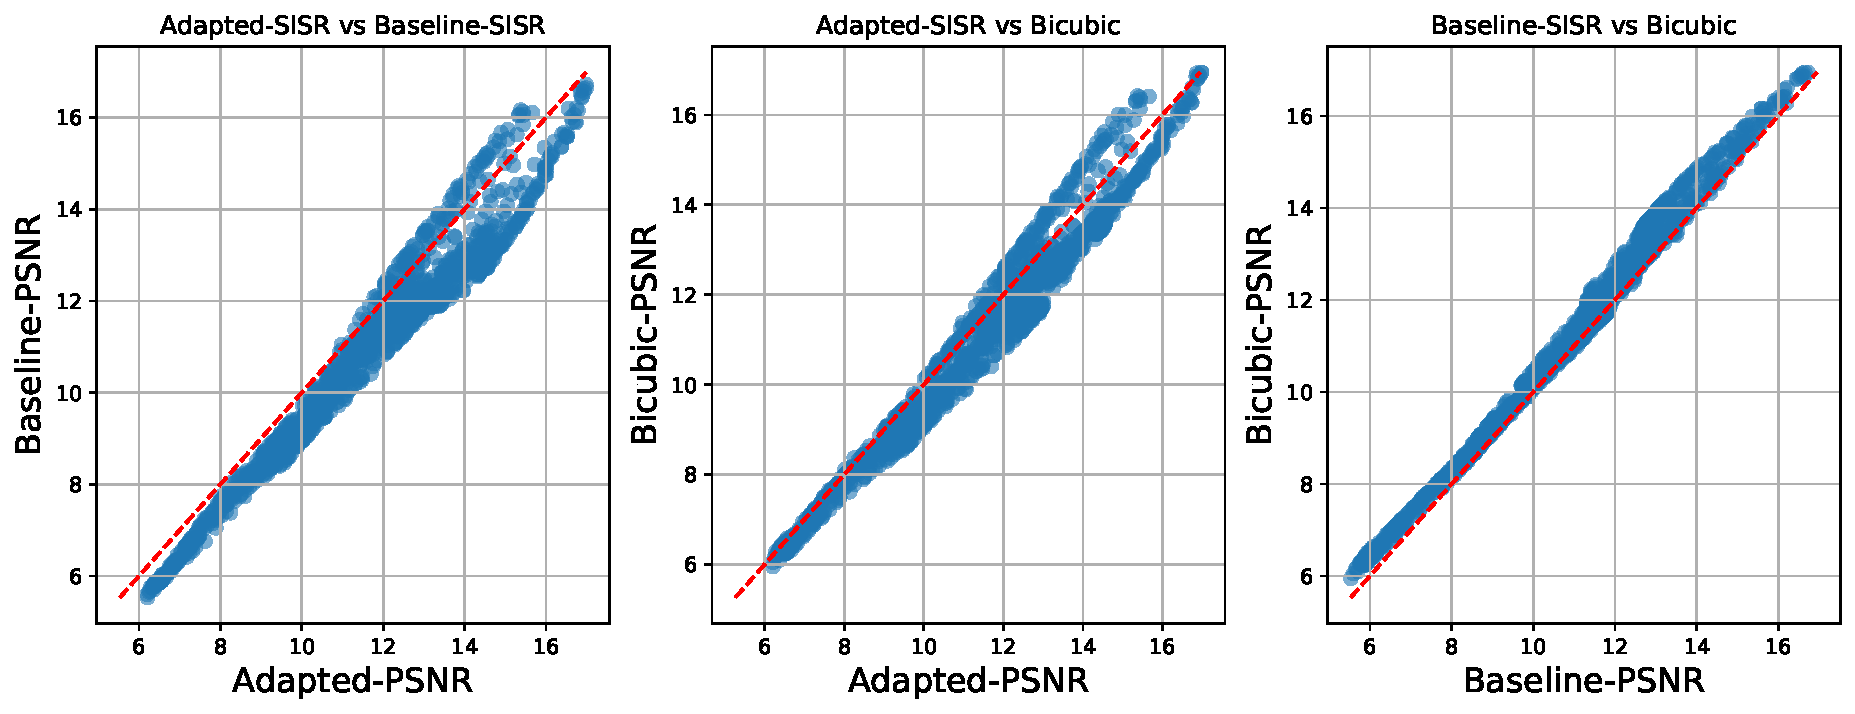
\includegraphics[width=\textwidth]{Includes/5-crossover-performance-scatter.pdf}
        \caption{Performance obtained by super resolving the FOREST-2 image using different models and comparing the result with ECOSTRESS.}
        \label{fig:5-crossover-fft-scatter}
    \end{figure}
        
\newpage
    